\documentclass[a4paper,10pt]{article}
\usepackage[pdftex]{color,graphicx}
\usepackage[pdftex, bookmarks, colorlinks]{hyperref}
\usepackage{longtable}
%\usepackage[all]{xy}
\addtolength{\textheight}{4cm}
\addtolength{\textwidth}{3cm}
\addtolength{\hoffset}{-3cm}
\addtolength{\voffset}{-3cm}

%opening
\title{Outcrossing}
\author{Yu Huang}

\begin{document}

\maketitle

\begin{abstract}

\end{abstract}

\tableofcontents

\section{Introduction}
Arabidopsis thaliana is a highly selfing species, with a very small portion resulting from outcrossing. An early electrophoretic study based on polymorphic enzymes\cite{Abbott1989} put the outcrossing rate to be less than 0.3\%.

Given the polymorphism data of 149 SNPs in 5720 strains, we set out to improve the estimate of the outcrossing rate in terms of accuracy and resolution.

\section{Data}
The strains were collected worldwide by numerous scientists including Eric Holub, Diane Myers, Justin Borevitz, Jon Agen, Megan Dunning (top 5 collectors) etc. The polymorphism data was generated by Sequenom, Inc. The 149 SNPs were picked based on an earlier work involving PCR sequencing\cite{Nordborg2005}. Figure~\ref{f1} shows the spacing of 149 SNPs.
Total 6389 runs of genotyping. 669 of them are technical duplications of 640 strains. So end up with 5720 strains based on ecotypeid. The 5720 strains were collected from around the world (Figure~\ref{fdata1} ).

Further, Remove 27 strains with all-NA data. Remove 14 strains with no GPS info.

So ends up with 5679 strains.

\subsection{tables showing intricate relationship between these strains}
\begin{figure}[H]
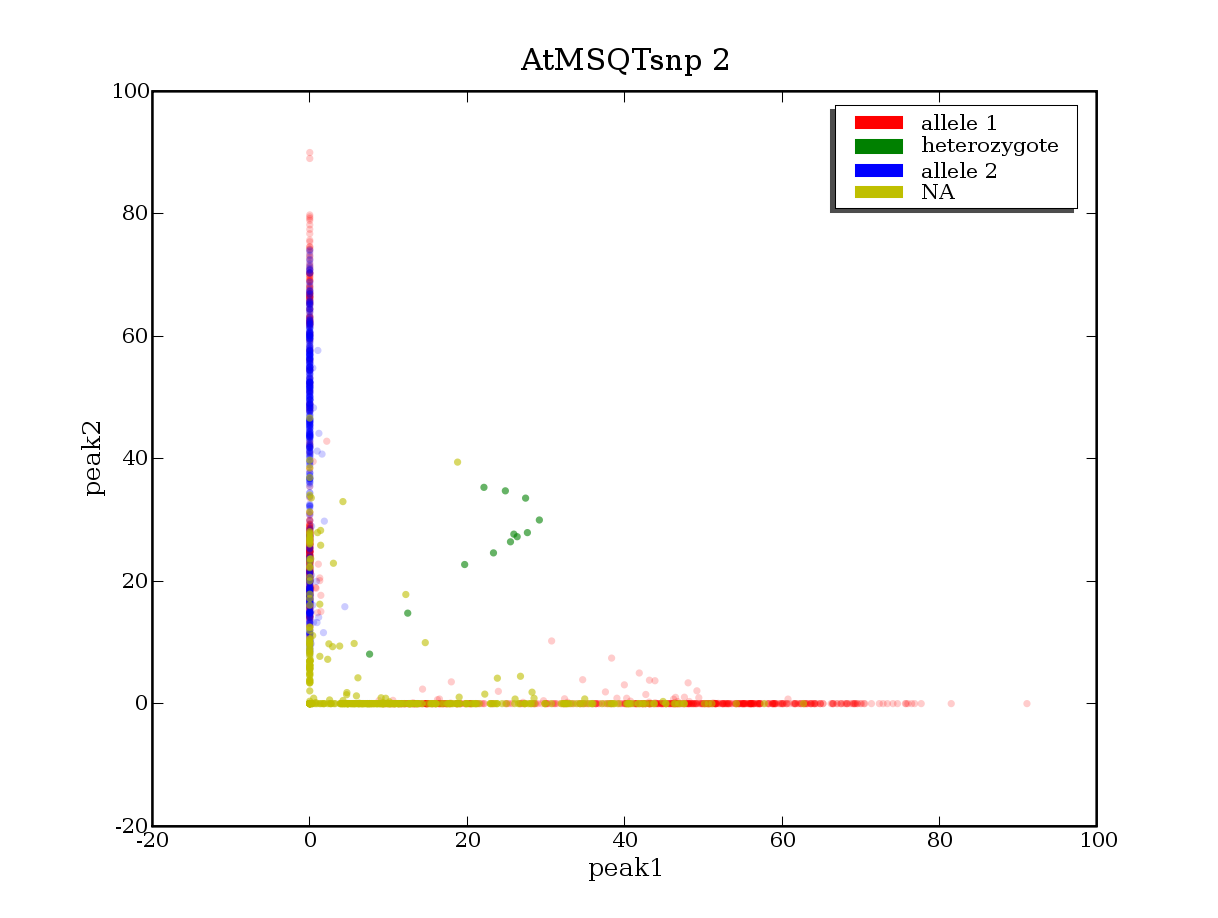
\includegraphics[width=0.5\textwidth]{figures/cluster_plot_AtMSQTsnp_2.png}
\caption{cluster plot for AtMSQTsnp 2.} \label{flAtMSQTsnp2}
\end{figure}
\begin{figure}[H]
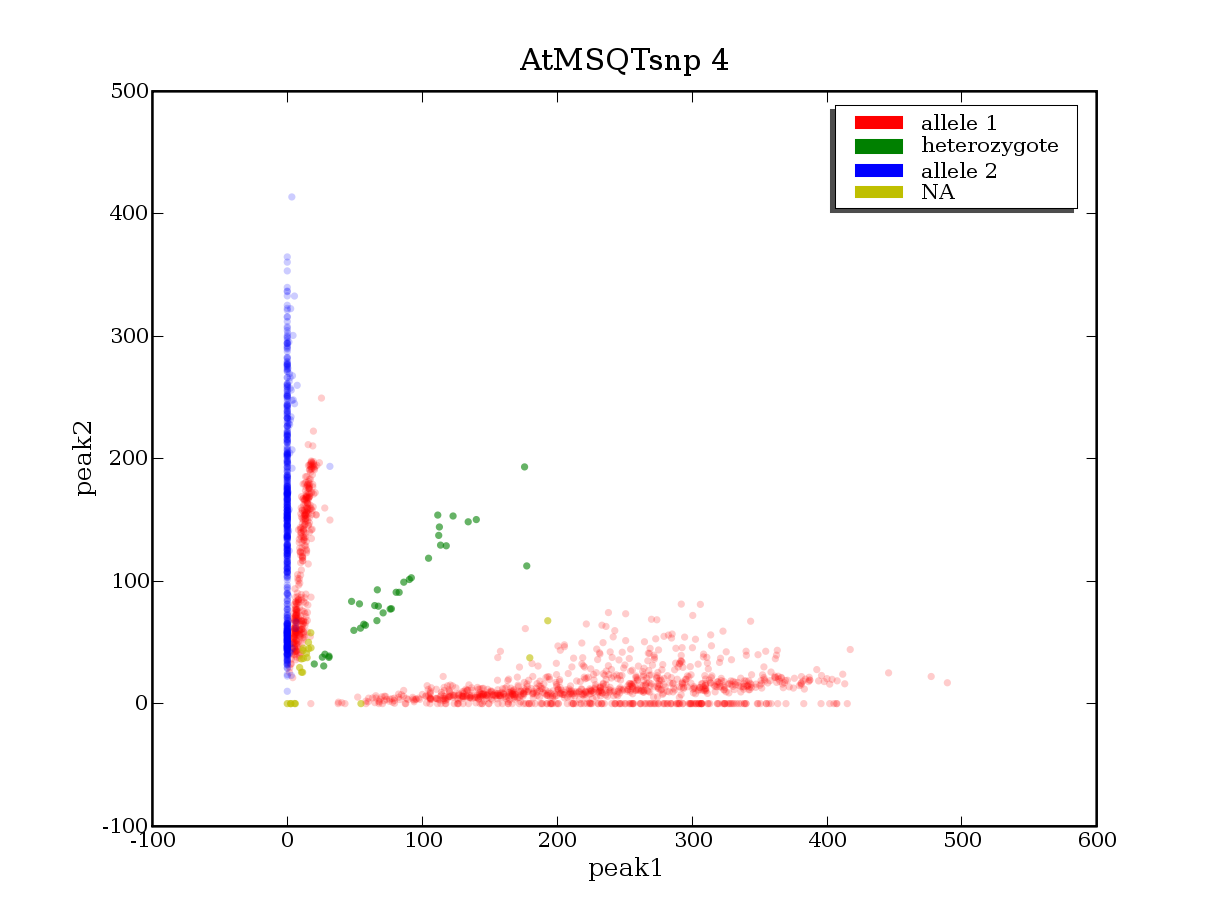
\includegraphics[width=0.5\textwidth]{figures/cluster_plot_AtMSQTsnp_4.png}
\caption{cluster plot for AtMSQTsnp 4.} \label{flAtMSQTsnp4}
\end{figure}
\begin{figure}[H]
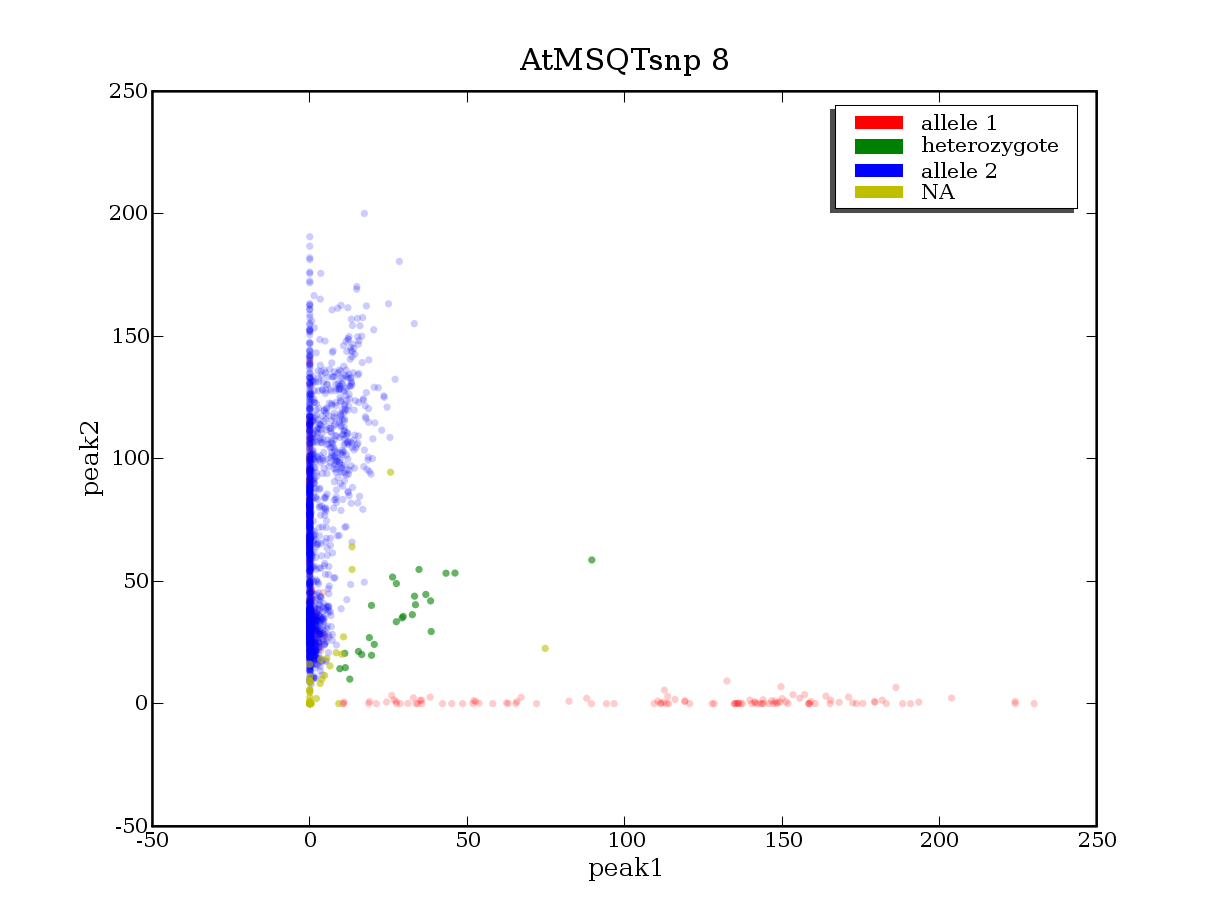
\includegraphics[width=0.5\textwidth]{figures/cluster_plot_AtMSQTsnp_8.png}
\caption{cluster plot for AtMSQTsnp 8.} \label{flAtMSQTsnp8}
\end{figure}
\begin{figure}[H]
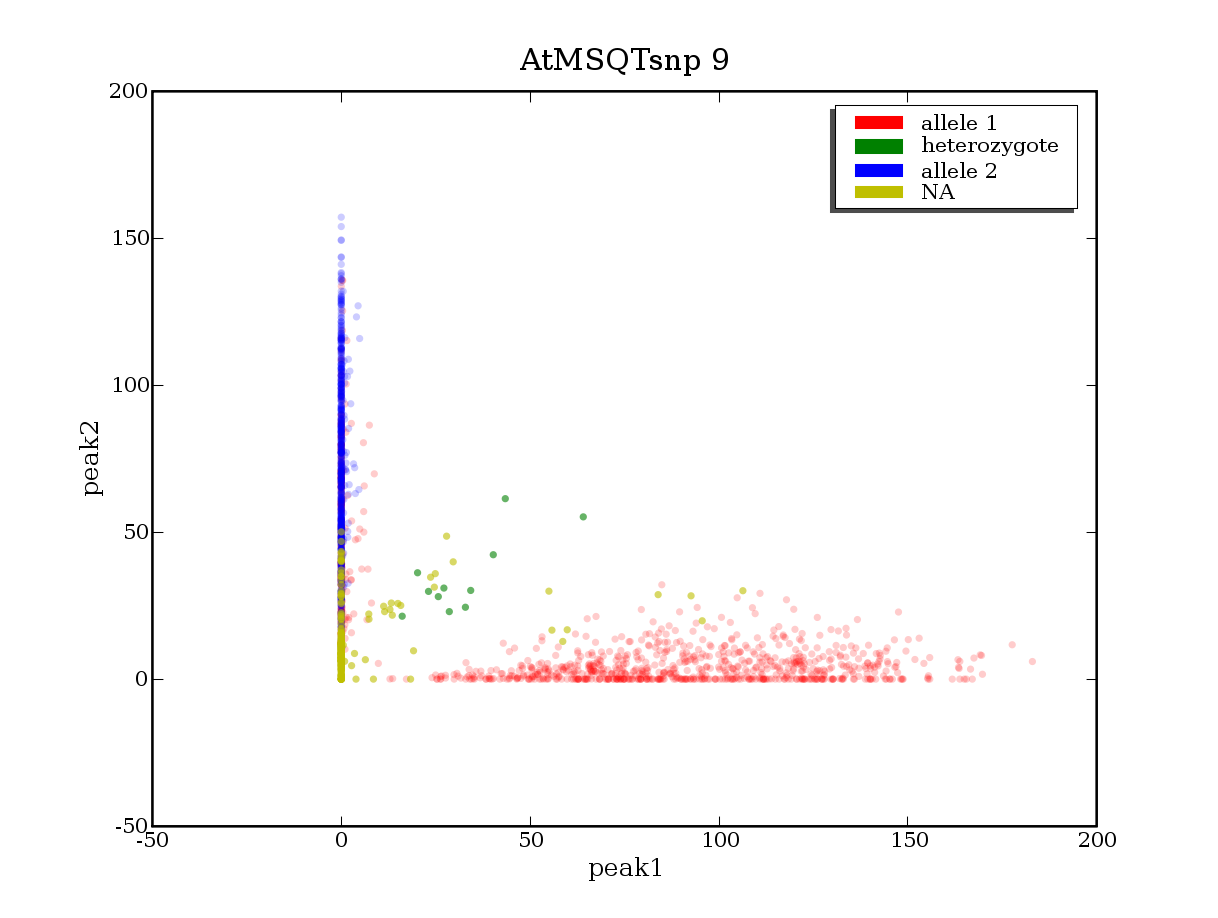
\includegraphics[width=0.5\textwidth]{figures/cluster_plot_AtMSQTsnp_9.png}
\caption{cluster plot for AtMSQTsnp 9.} \label{flAtMSQTsnp9}
\end{figure}
\begin{figure}[H]
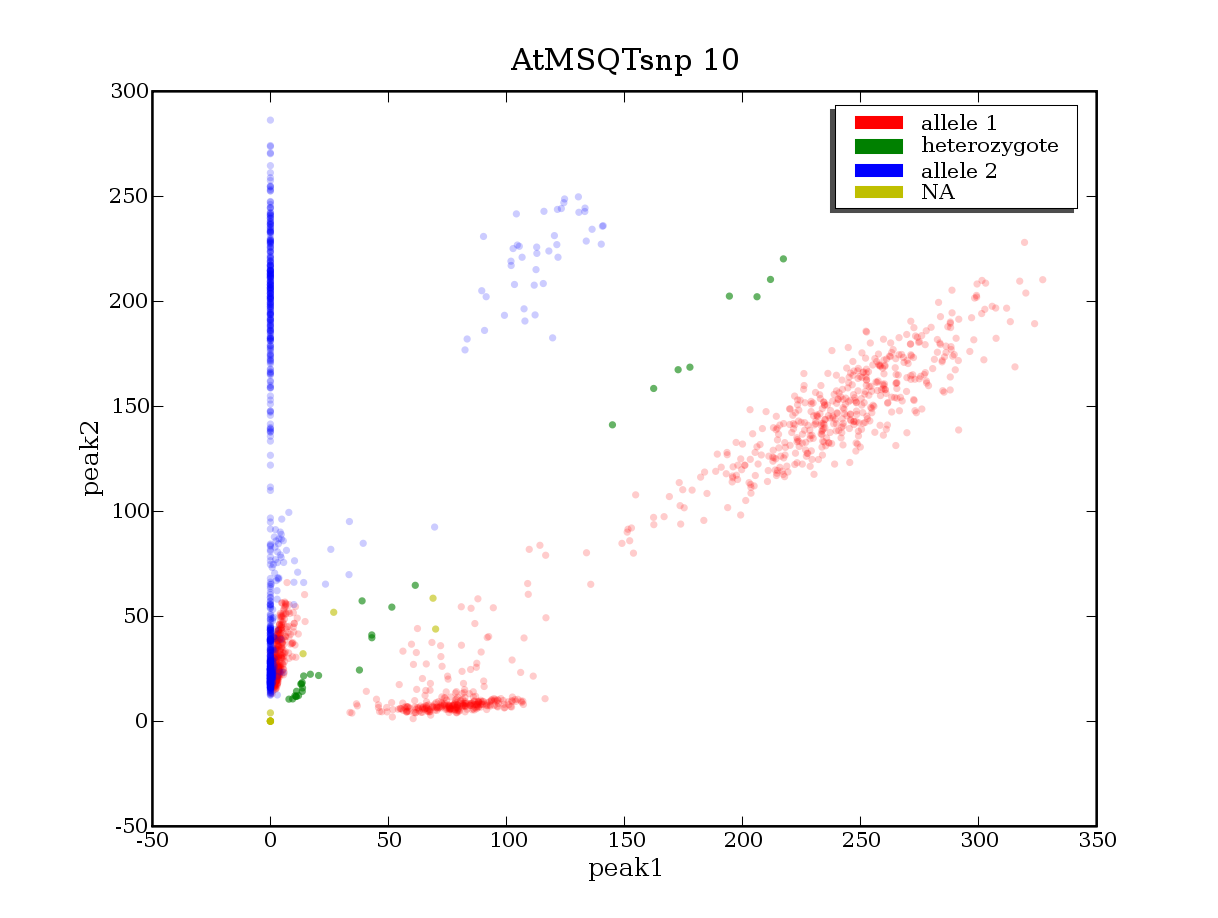
\includegraphics[width=0.5\textwidth]{figures/cluster_plot_AtMSQTsnp_10.png}
\caption{cluster plot for AtMSQTsnp 10.} \label{flAtMSQTsnp10}
\end{figure}
\begin{figure}[H]
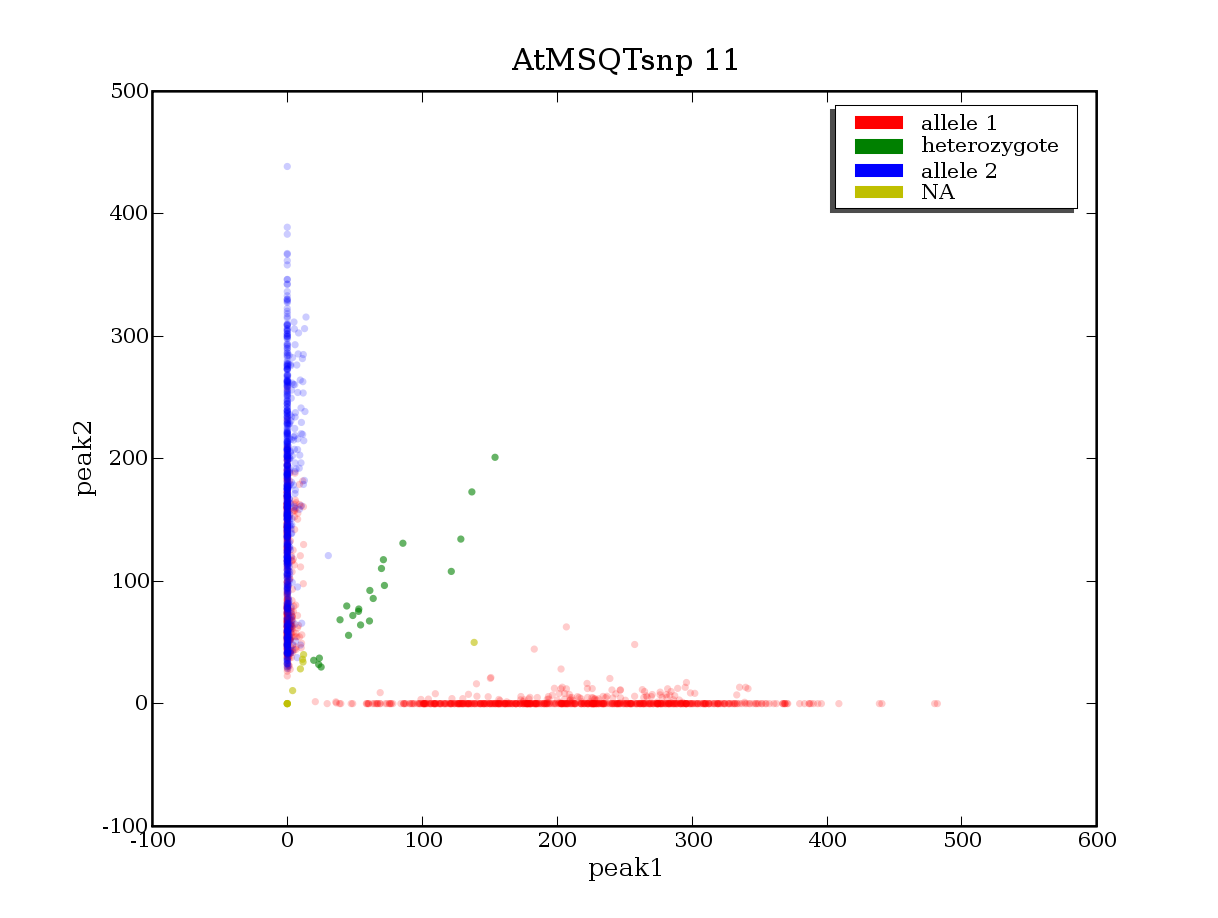
\includegraphics[width=0.5\textwidth]{figures/cluster_plot_AtMSQTsnp_11.png}
\caption{cluster plot for AtMSQTsnp 11.} \label{flAtMSQTsnp11}
\end{figure}
\begin{figure}[H]
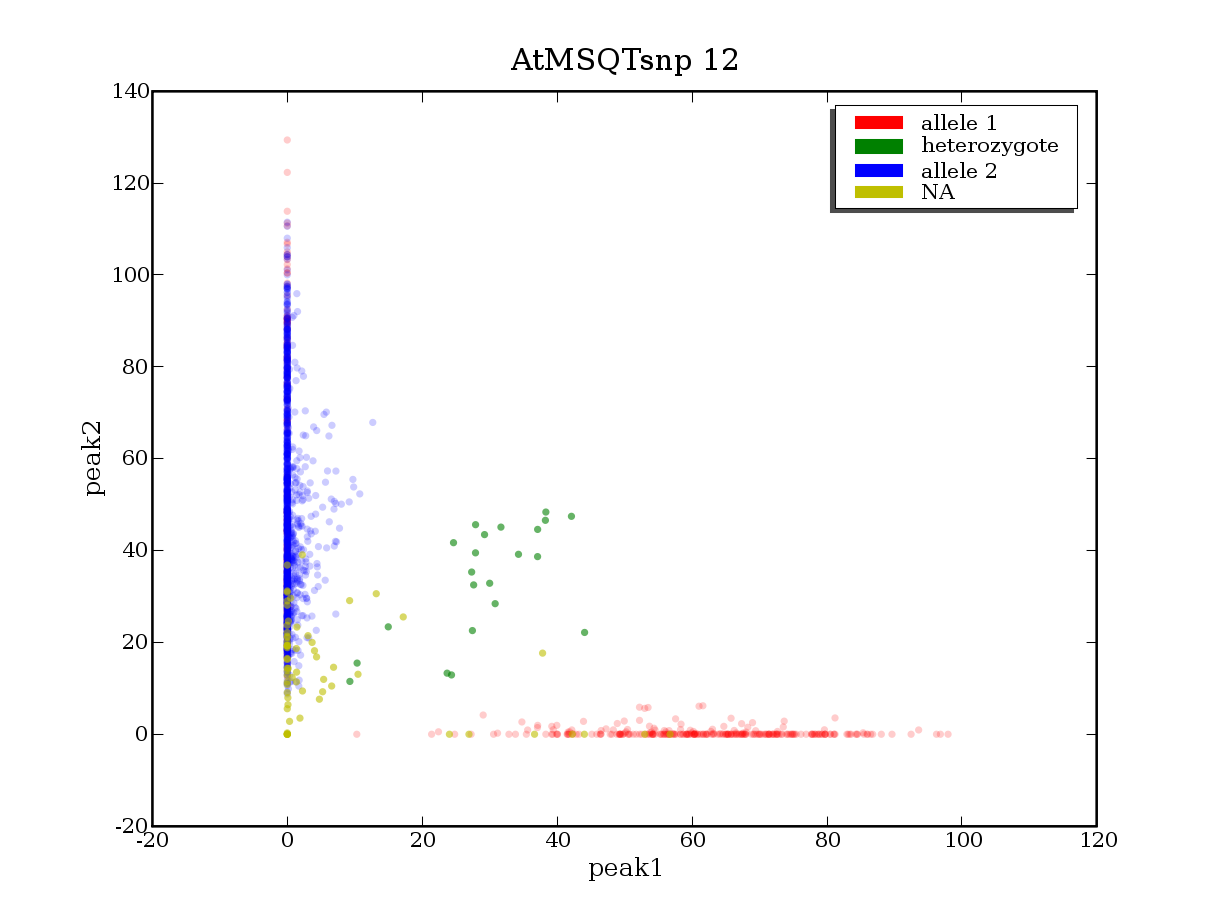
\includegraphics[width=0.5\textwidth]{figures/cluster_plot_AtMSQTsnp_12.png}
\caption{cluster plot for AtMSQTsnp 12.} \label{flAtMSQTsnp12}
\end{figure}
\begin{figure}[H]
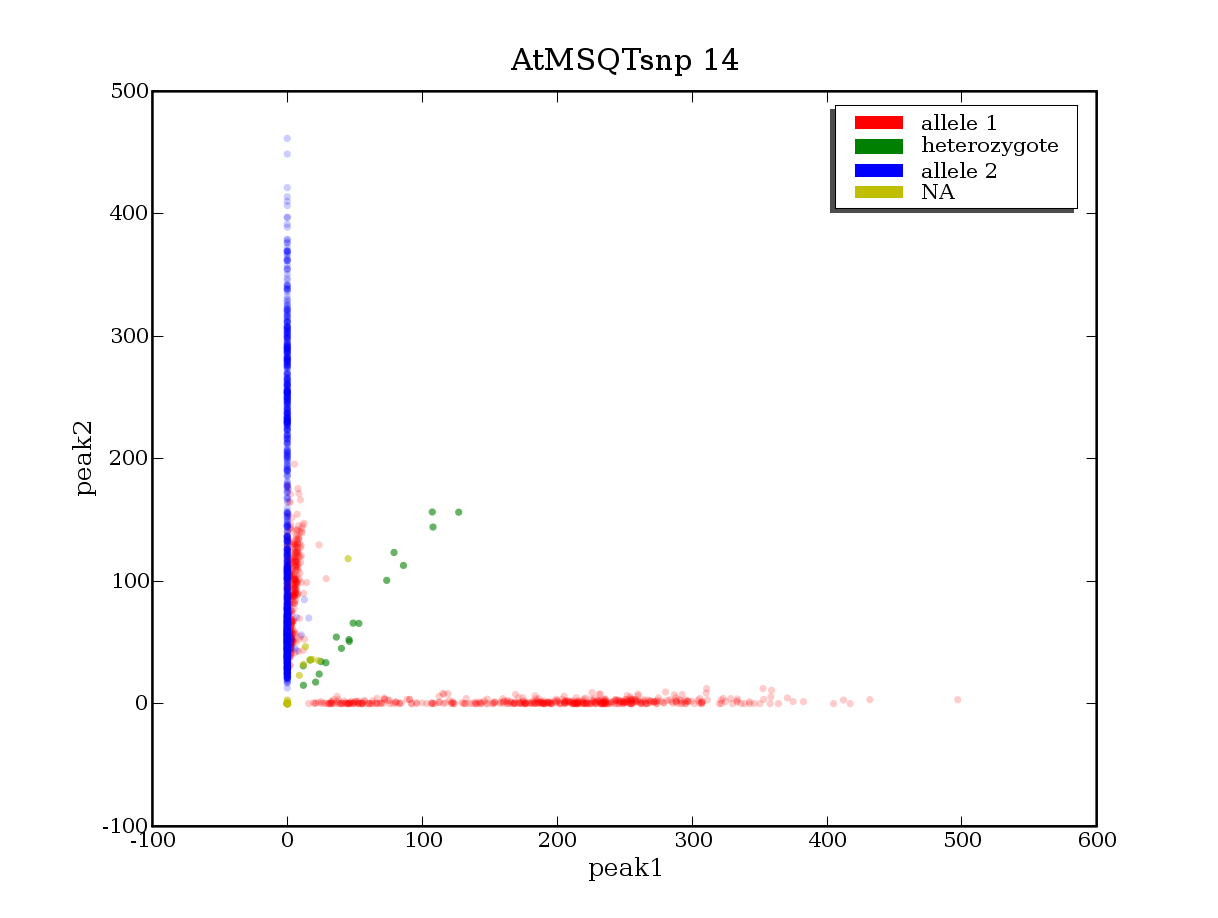
\includegraphics[width=0.5\textwidth]{figures/cluster_plot_AtMSQTsnp_14.png}
\caption{cluster plot for AtMSQTsnp 14.} \label{flAtMSQTsnp14}
\end{figure}
\begin{figure}[H]
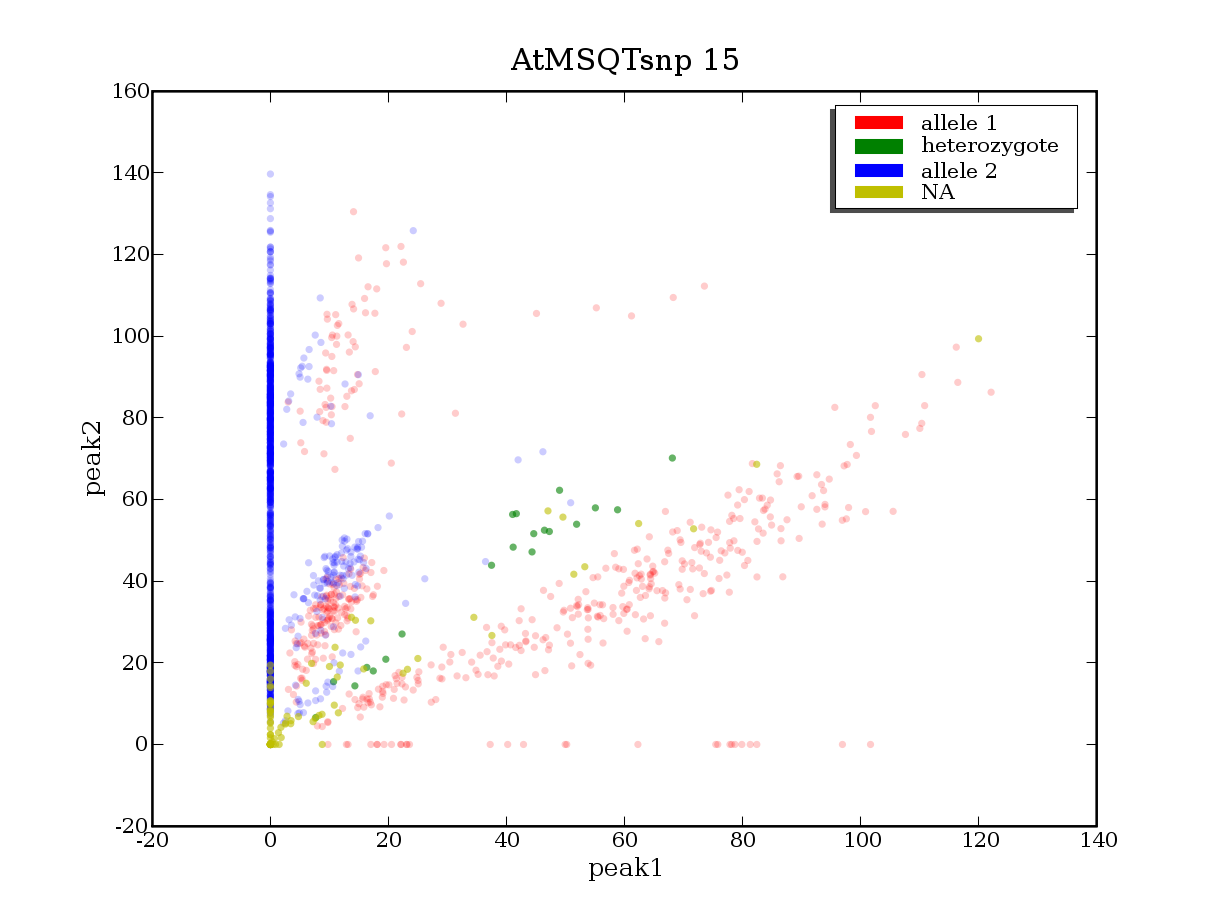
\includegraphics[width=0.5\textwidth]{figures/cluster_plot_AtMSQTsnp_15.png}
\caption{cluster plot for AtMSQTsnp 15.} \label{flAtMSQTsnp15}
\end{figure}
\begin{figure}[H]
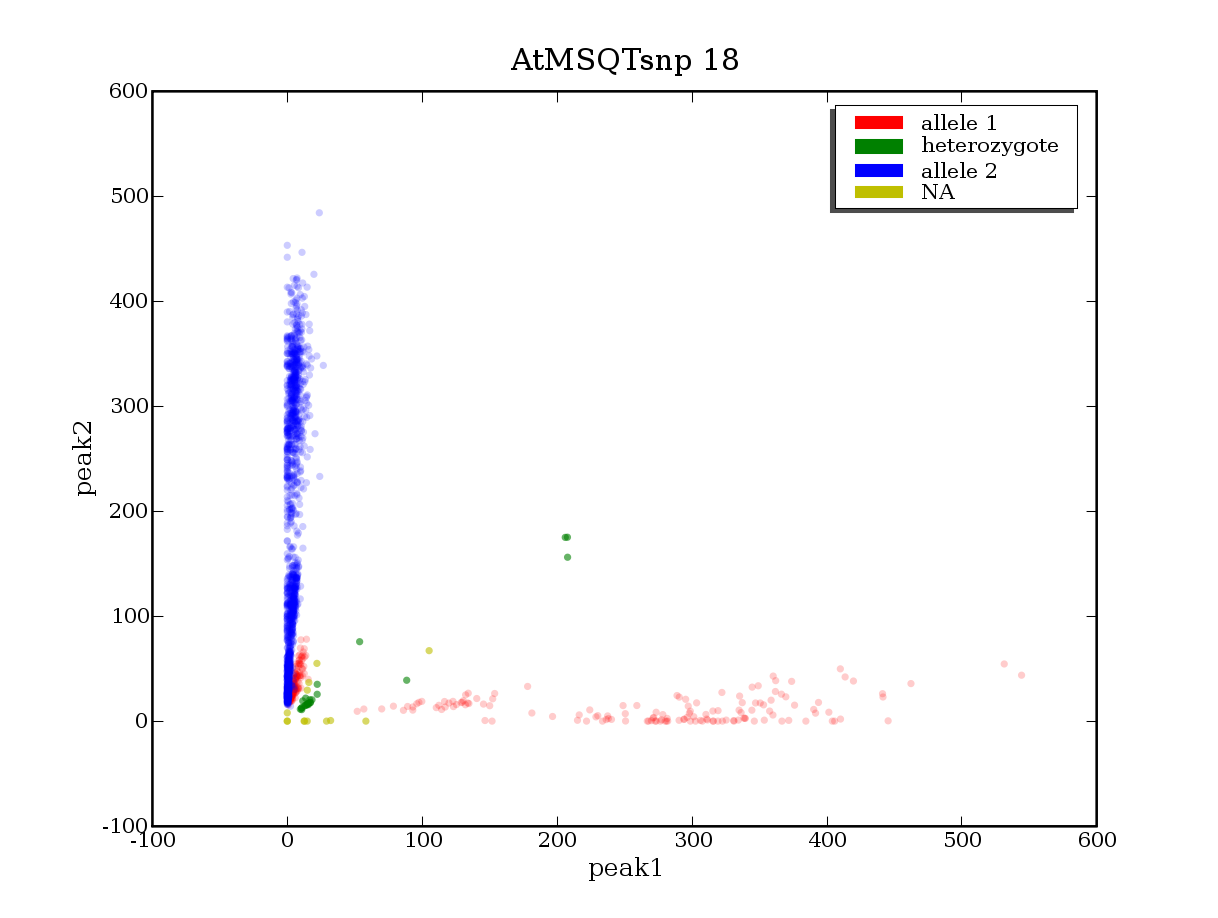
\includegraphics[width=0.5\textwidth]{figures/cluster_plot_AtMSQTsnp_18.png}
\caption{cluster plot for AtMSQTsnp 18.} \label{flAtMSQTsnp18}
\end{figure}
\begin{figure}[H]
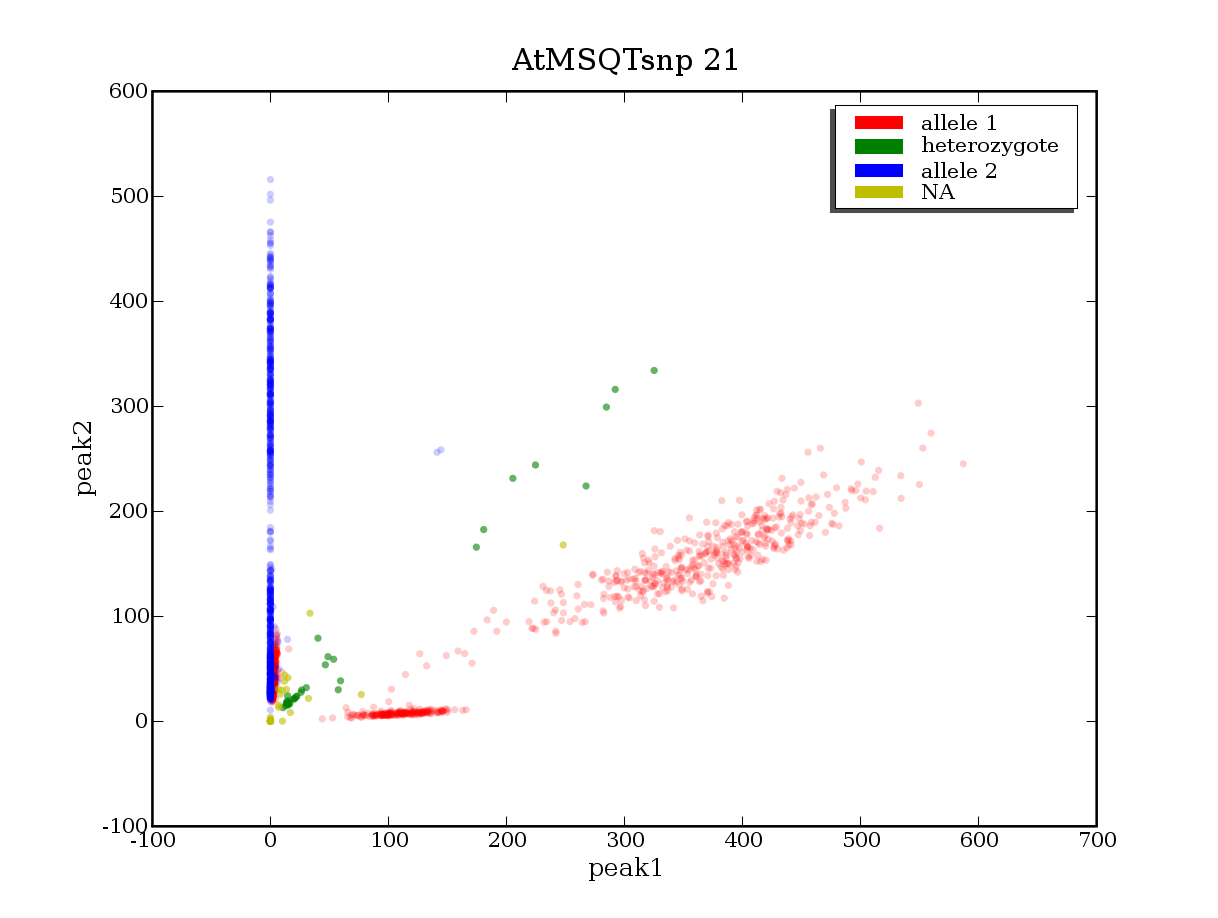
\includegraphics[width=0.5\textwidth]{figures/cluster_plot_AtMSQTsnp_21.png}
\caption{cluster plot for AtMSQTsnp 21.} \label{flAtMSQTsnp21}
\end{figure}
\begin{figure}[H]
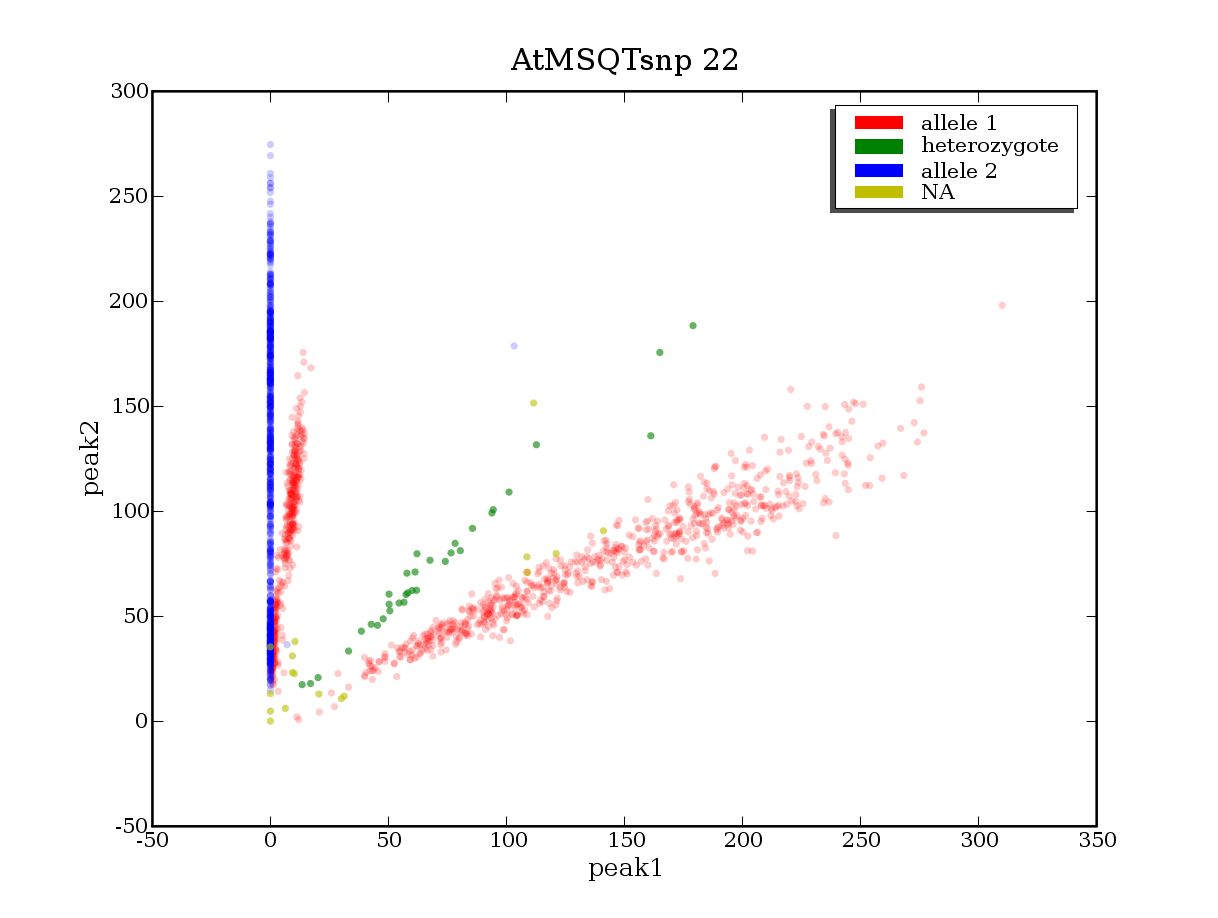
\includegraphics[width=0.5\textwidth]{figures/cluster_plot_AtMSQTsnp_22.png}
\caption{cluster plot for AtMSQTsnp 22.} \label{flAtMSQTsnp22}
\end{figure}
\begin{figure}[H]
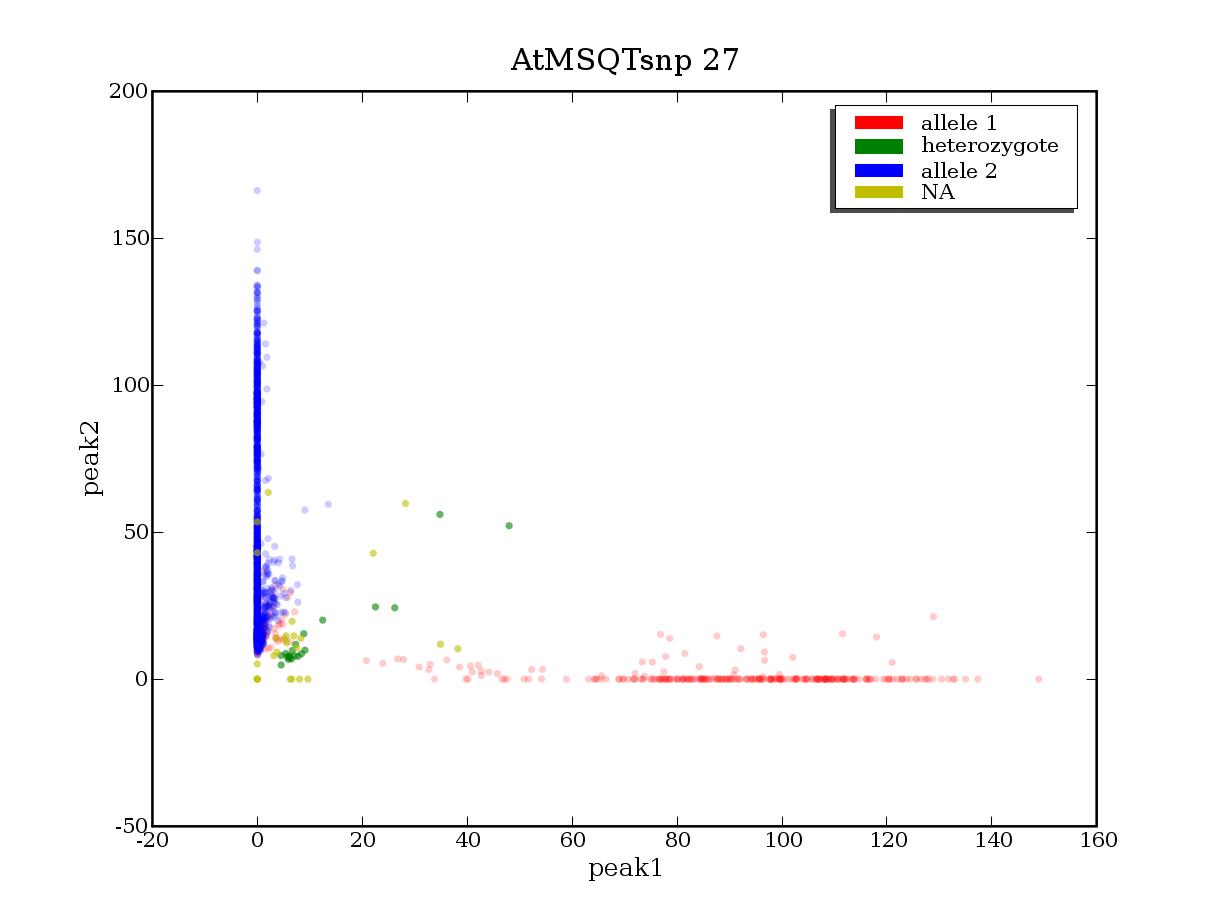
\includegraphics[width=0.5\textwidth]{figures/cluster_plot_AtMSQTsnp_27.png}
\caption{cluster plot for AtMSQTsnp 27.} \label{flAtMSQTsnp27}
\end{figure}
\begin{figure}[H]
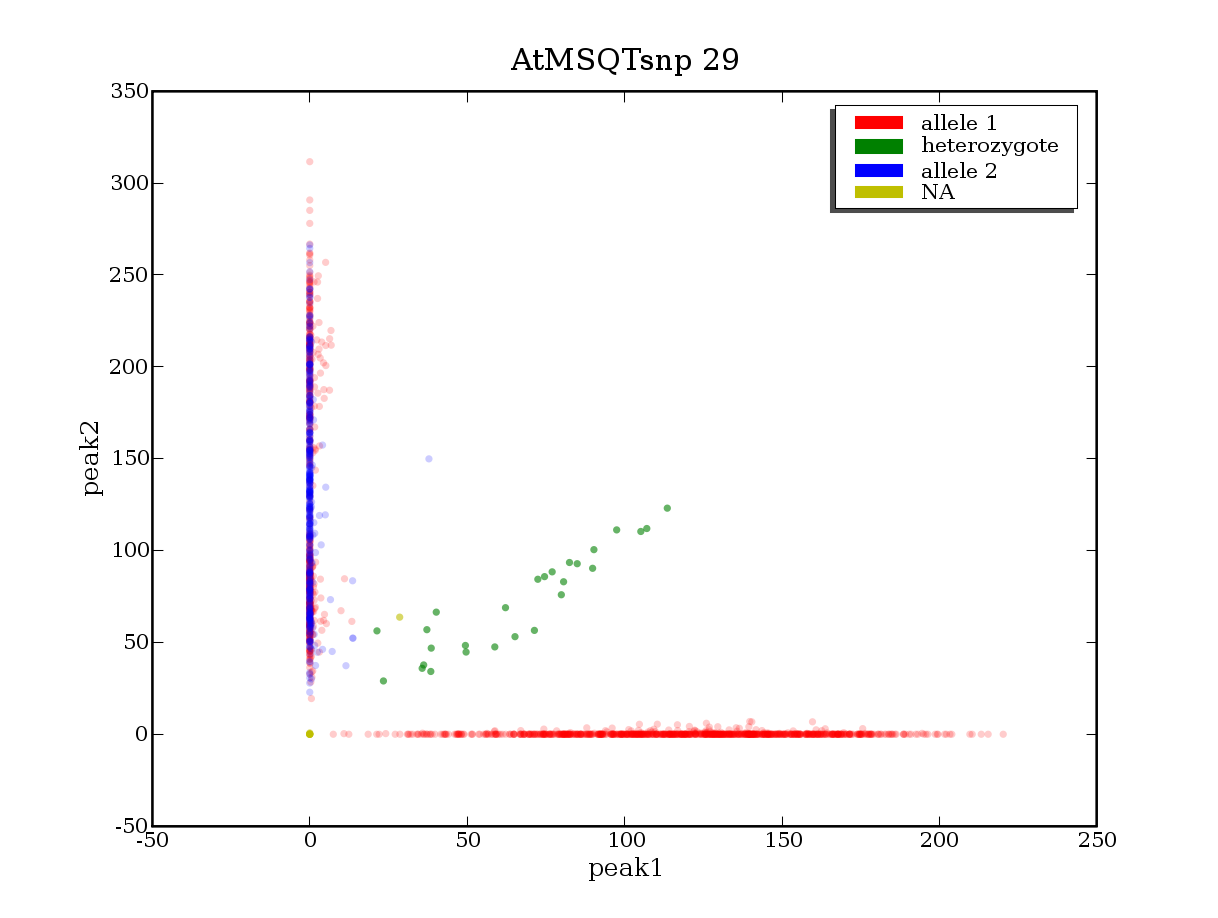
\includegraphics[width=0.5\textwidth]{figures/cluster_plot_AtMSQTsnp_29.png}
\caption{cluster plot for AtMSQTsnp 29.} \label{flAtMSQTsnp29}
\end{figure}
\begin{figure}[H]
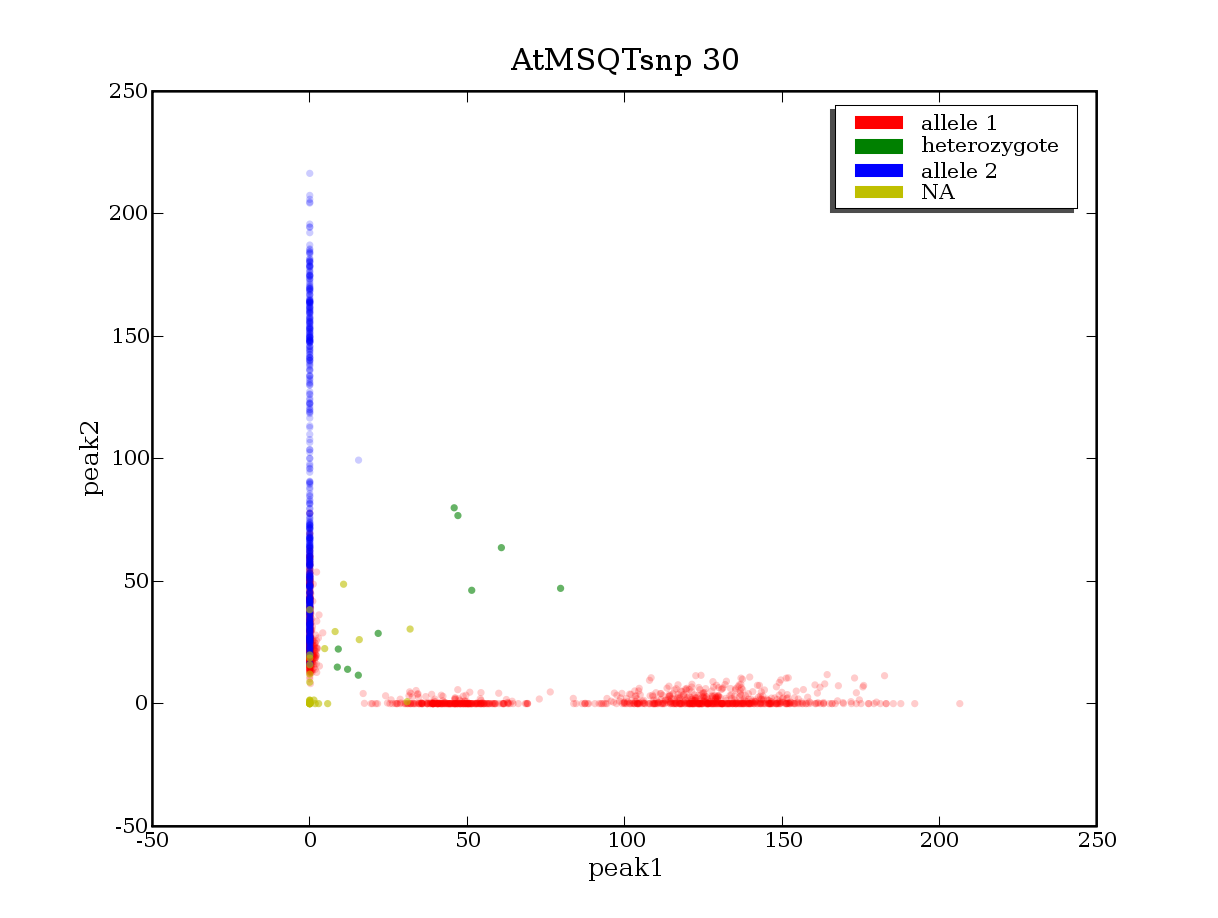
\includegraphics[width=0.5\textwidth]{figures/cluster_plot_AtMSQTsnp_30.png}
\caption{cluster plot for AtMSQTsnp 30.} \label{flAtMSQTsnp30}
\end{figure}
\begin{figure}[H]
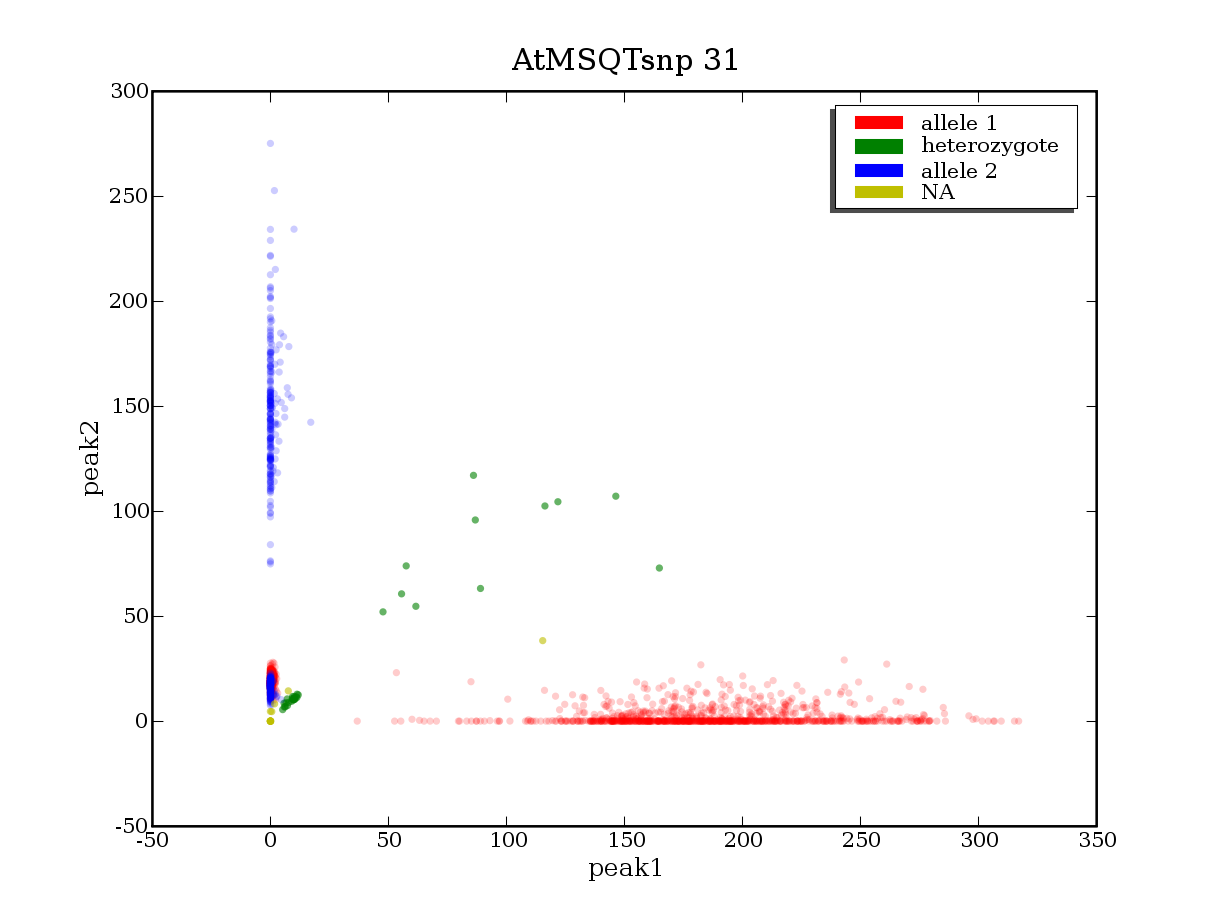
\includegraphics[width=0.5\textwidth]{figures/cluster_plot_AtMSQTsnp_31.png}
\caption{cluster plot for AtMSQTsnp 31.} \label{flAtMSQTsnp31}
\end{figure}
\begin{figure}[H]
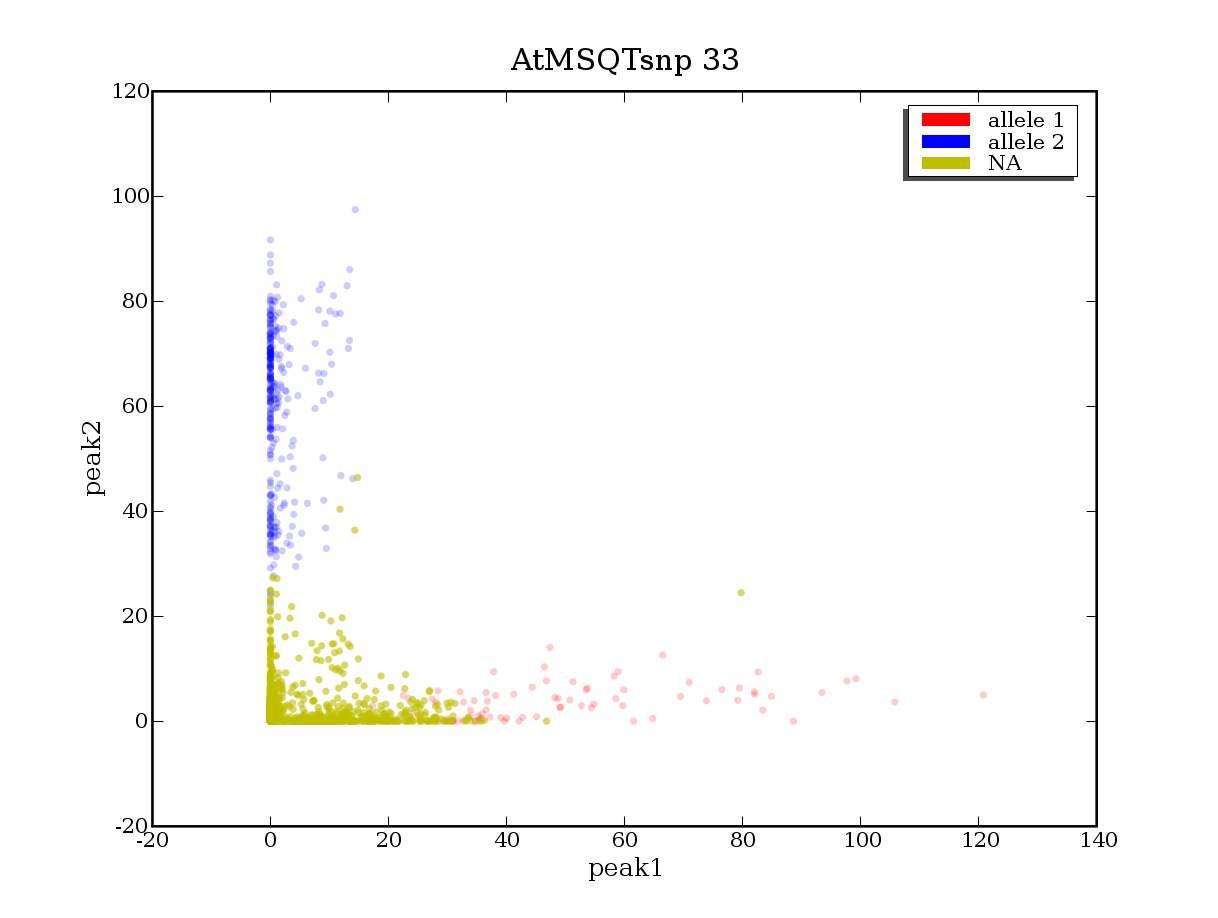
\includegraphics[width=0.5\textwidth]{figures/cluster_plot_AtMSQTsnp_33.png}
\caption{cluster plot for AtMSQTsnp 33.} \label{flAtMSQTsnp33}
\end{figure}
\begin{figure}[H]
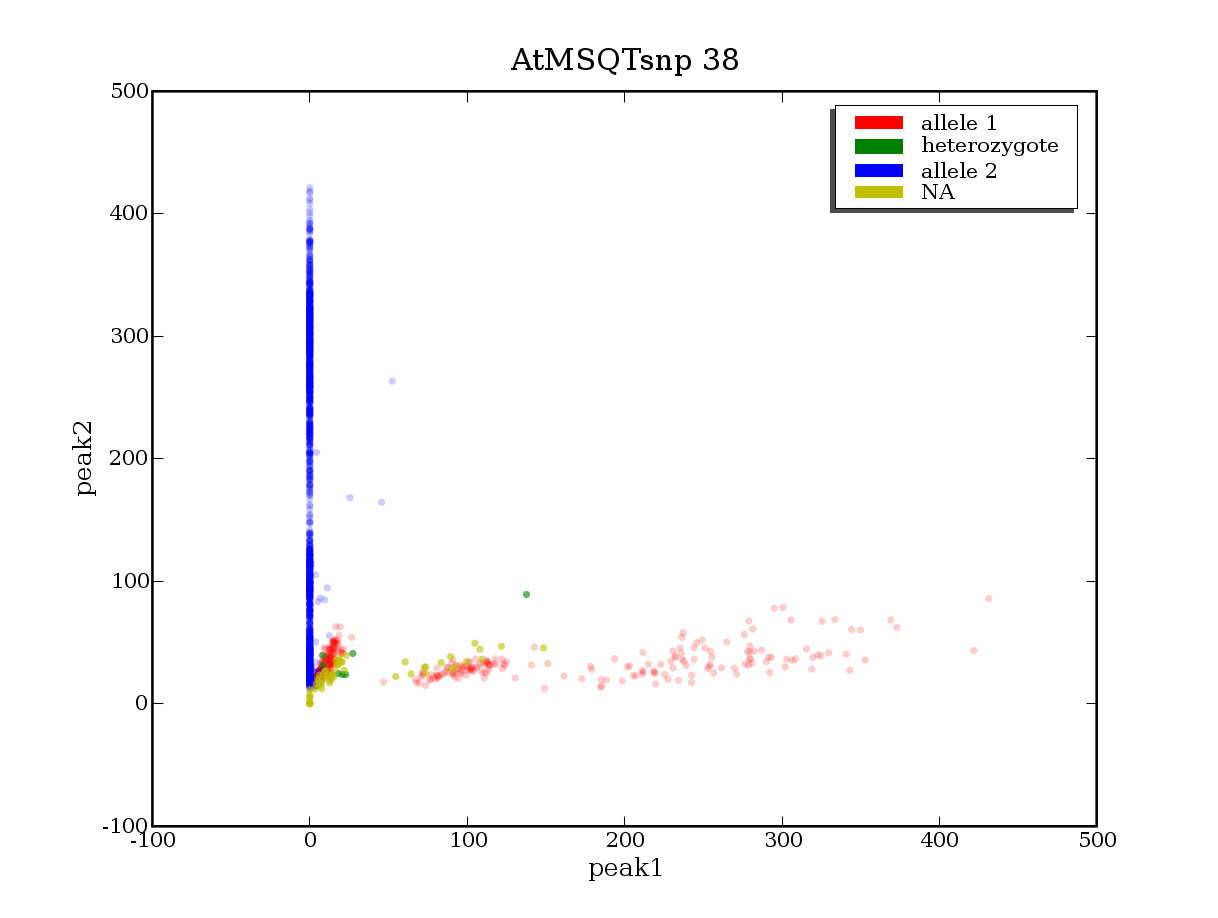
\includegraphics[width=0.5\textwidth]{figures/cluster_plot_AtMSQTsnp_38.png}
\caption{cluster plot for AtMSQTsnp 38.} \label{flAtMSQTsnp38}
\end{figure}
\begin{figure}[H]
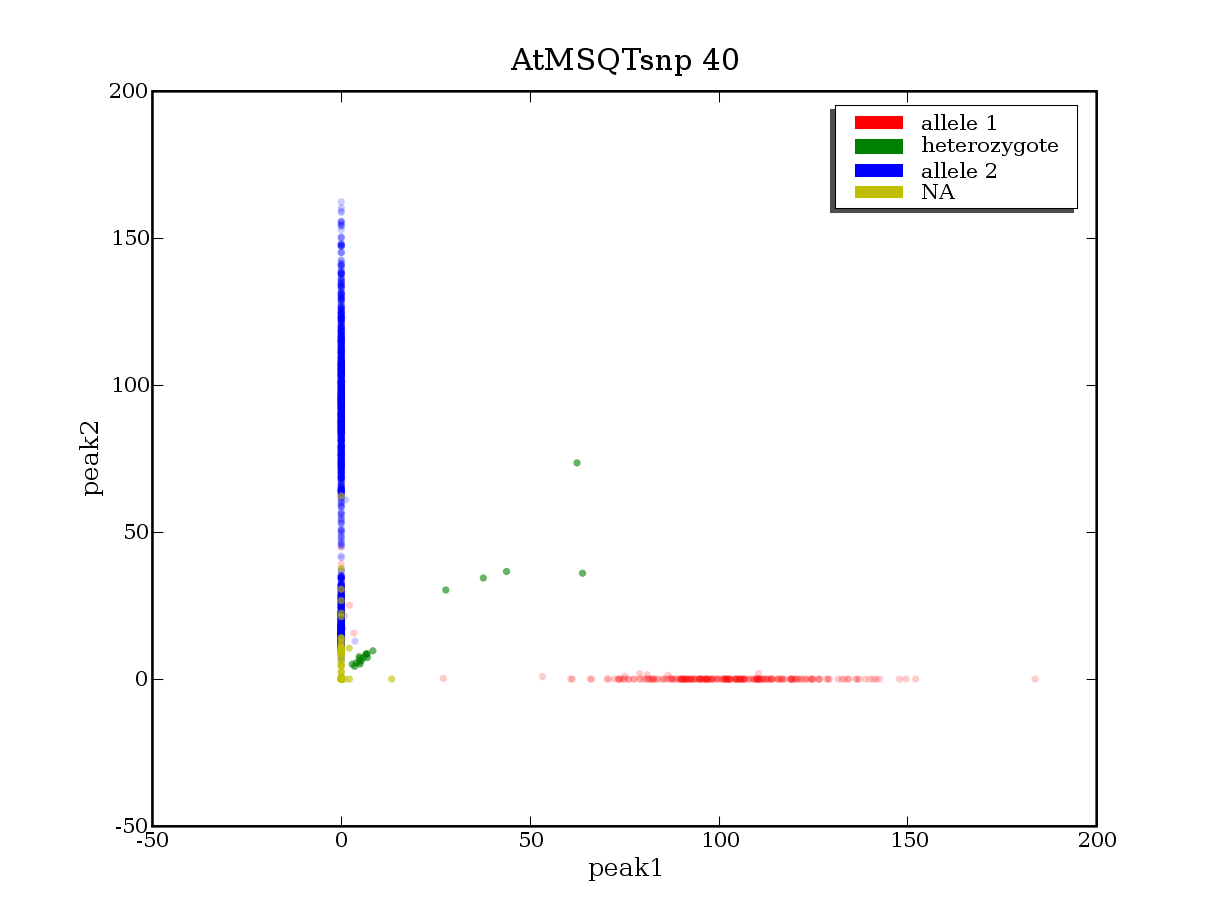
\includegraphics[width=0.5\textwidth]{figures/cluster_plot_AtMSQTsnp_40.png}
\caption{cluster plot for AtMSQTsnp 40.} \label{flAtMSQTsnp40}
\end{figure}
\begin{figure}[H]
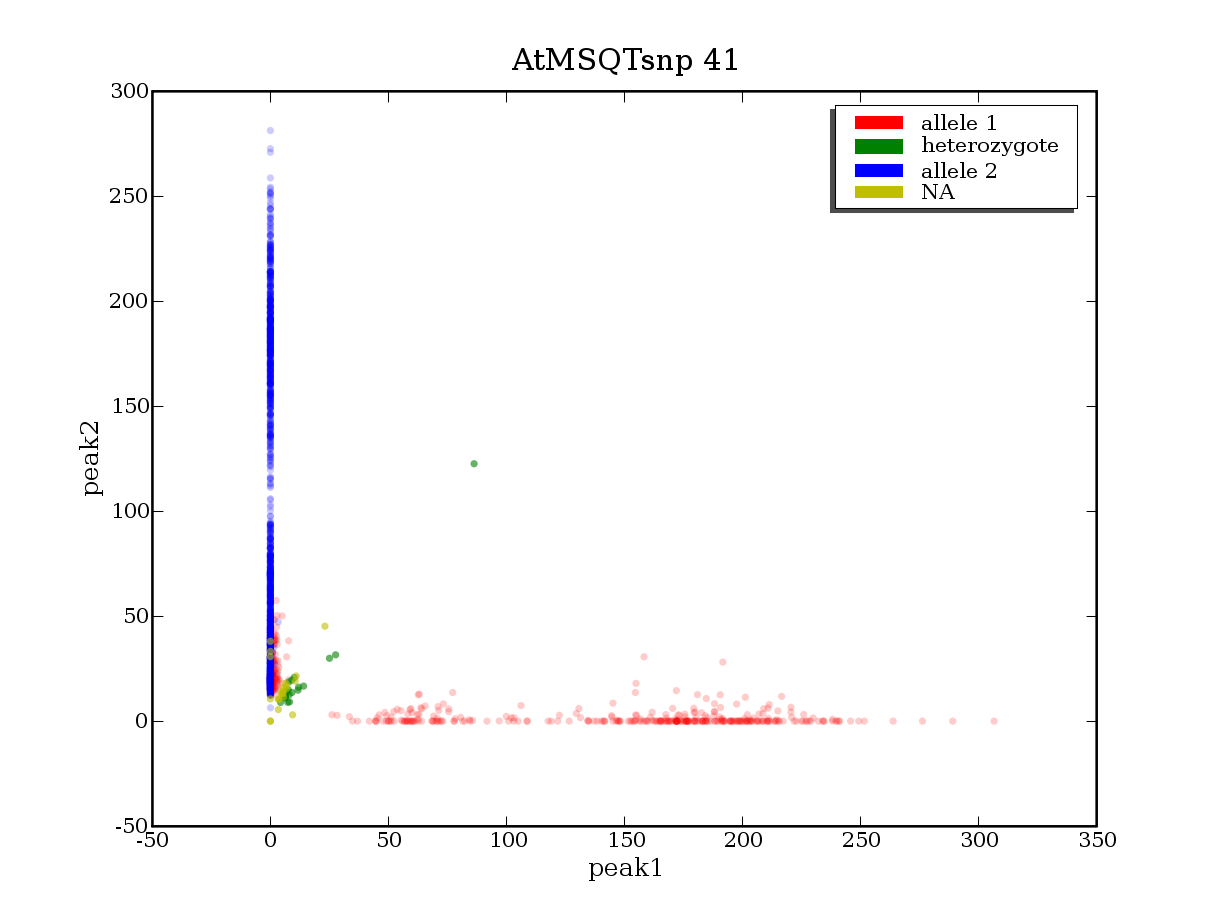
\includegraphics[width=0.5\textwidth]{figures/cluster_plot_AtMSQTsnp_41.png}
\caption{cluster plot for AtMSQTsnp 41.} \label{flAtMSQTsnp41}
\end{figure}
\begin{figure}[H]
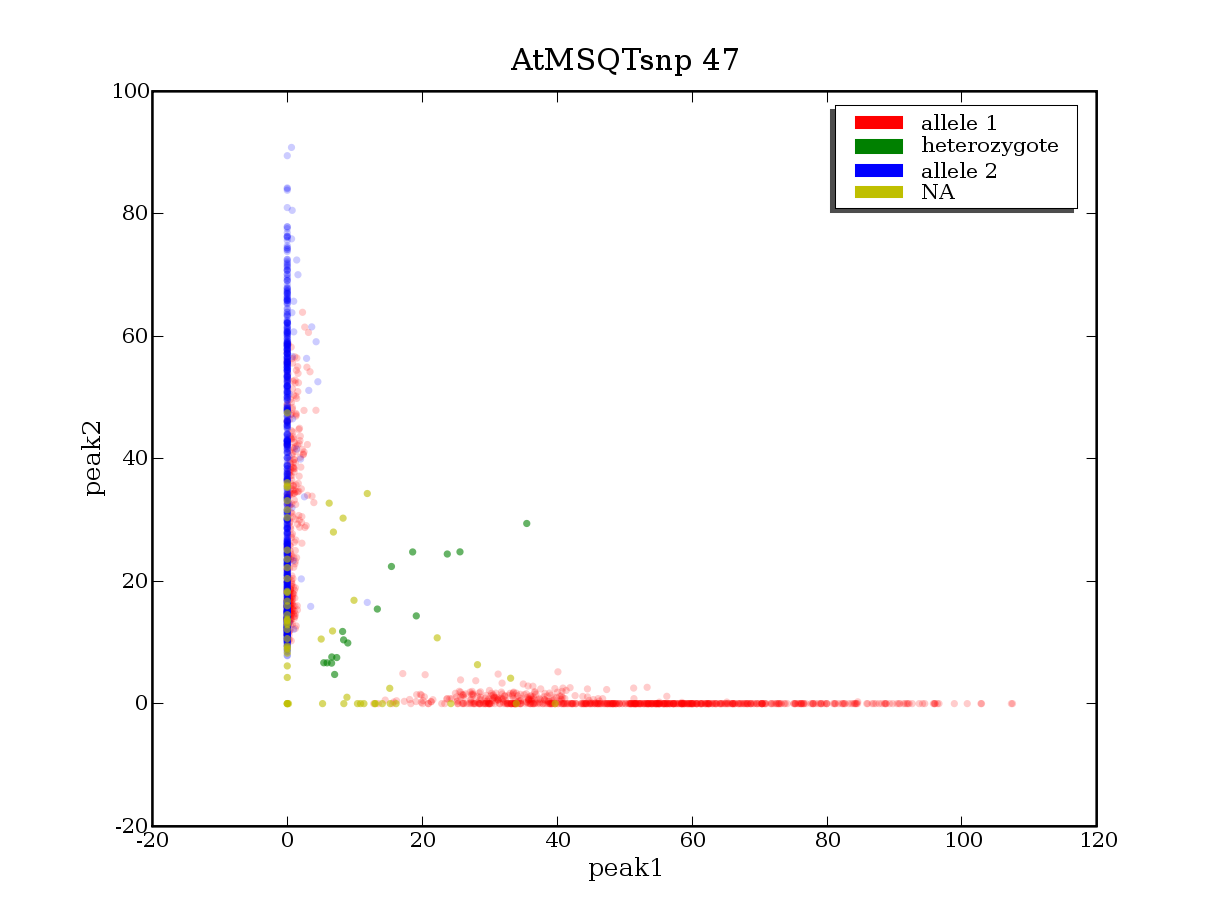
\includegraphics[width=0.5\textwidth]{figures/cluster_plot_AtMSQTsnp_47.png}
\caption{cluster plot for AtMSQTsnp 47.} \label{flAtMSQTsnp47}
\end{figure}
\begin{figure}[H]
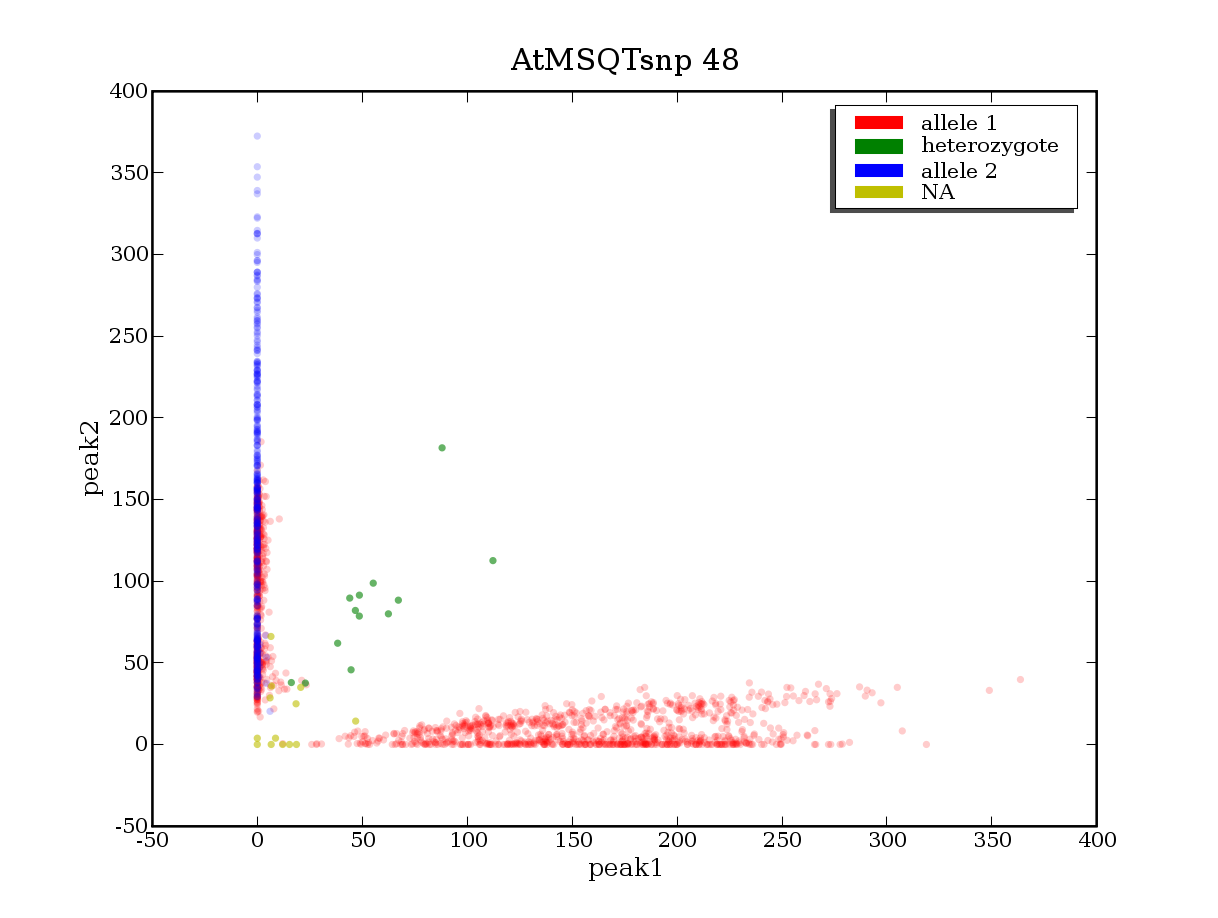
\includegraphics[width=0.5\textwidth]{figures/cluster_plot_AtMSQTsnp_48.png}
\caption{cluster plot for AtMSQTsnp 48.} \label{flAtMSQTsnp48}
\end{figure}
\begin{figure}[H]
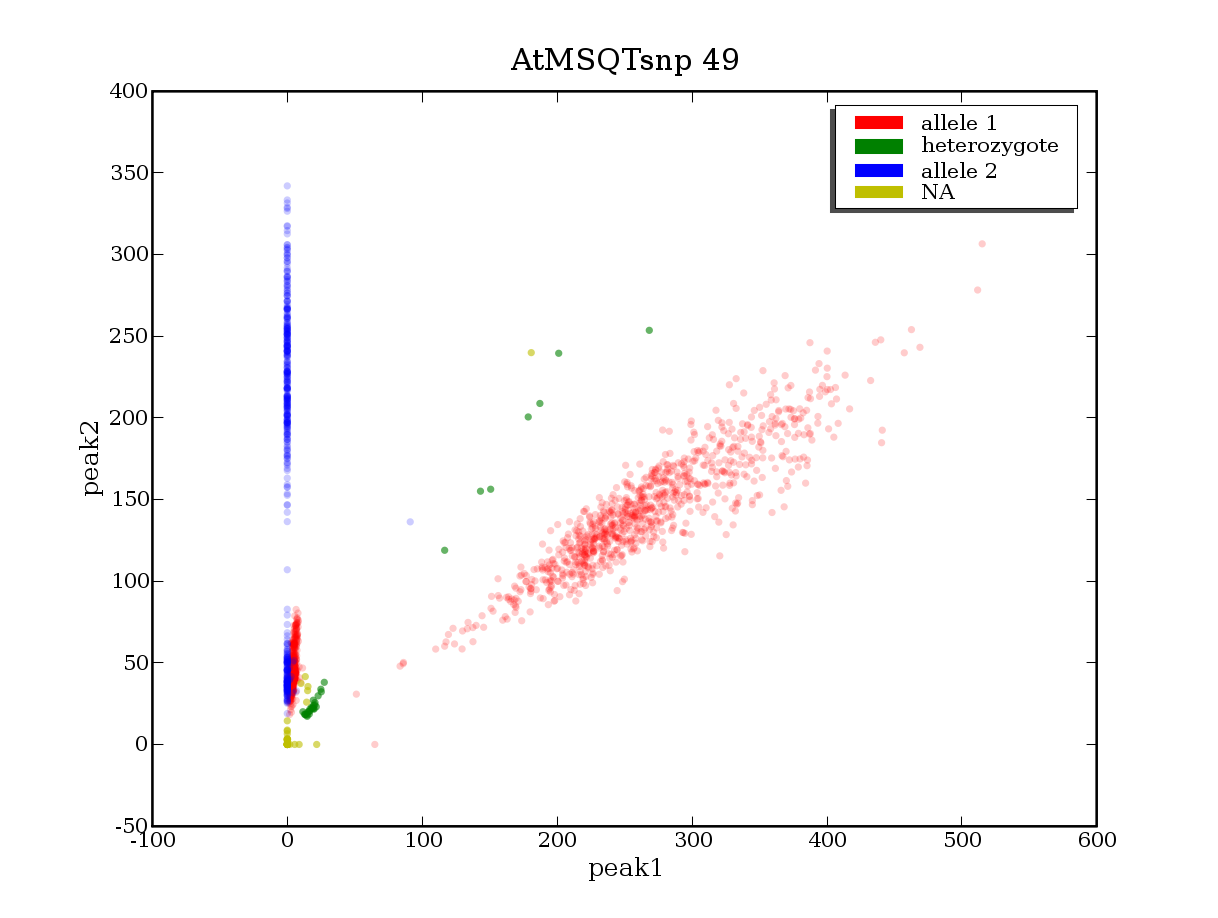
\includegraphics[width=0.5\textwidth]{figures/cluster_plot_AtMSQTsnp_49.png}
\caption{cluster plot for AtMSQTsnp 49.} \label{flAtMSQTsnp49}
\end{figure}
\begin{figure}[H]
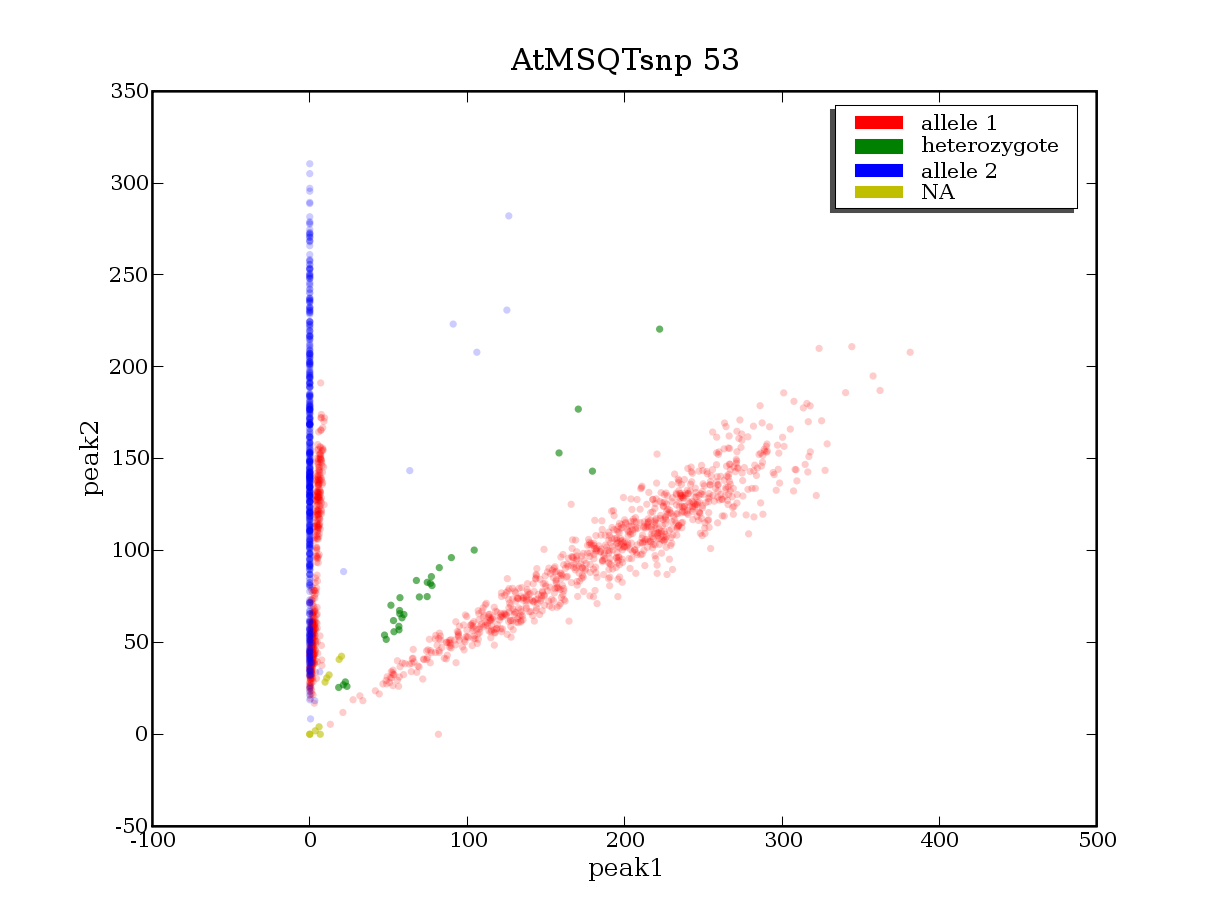
\includegraphics[width=0.5\textwidth]{figures/cluster_plot_AtMSQTsnp_53.png}
\caption{cluster plot for AtMSQTsnp 53.} \label{flAtMSQTsnp53}
\end{figure}
\begin{figure}[H]
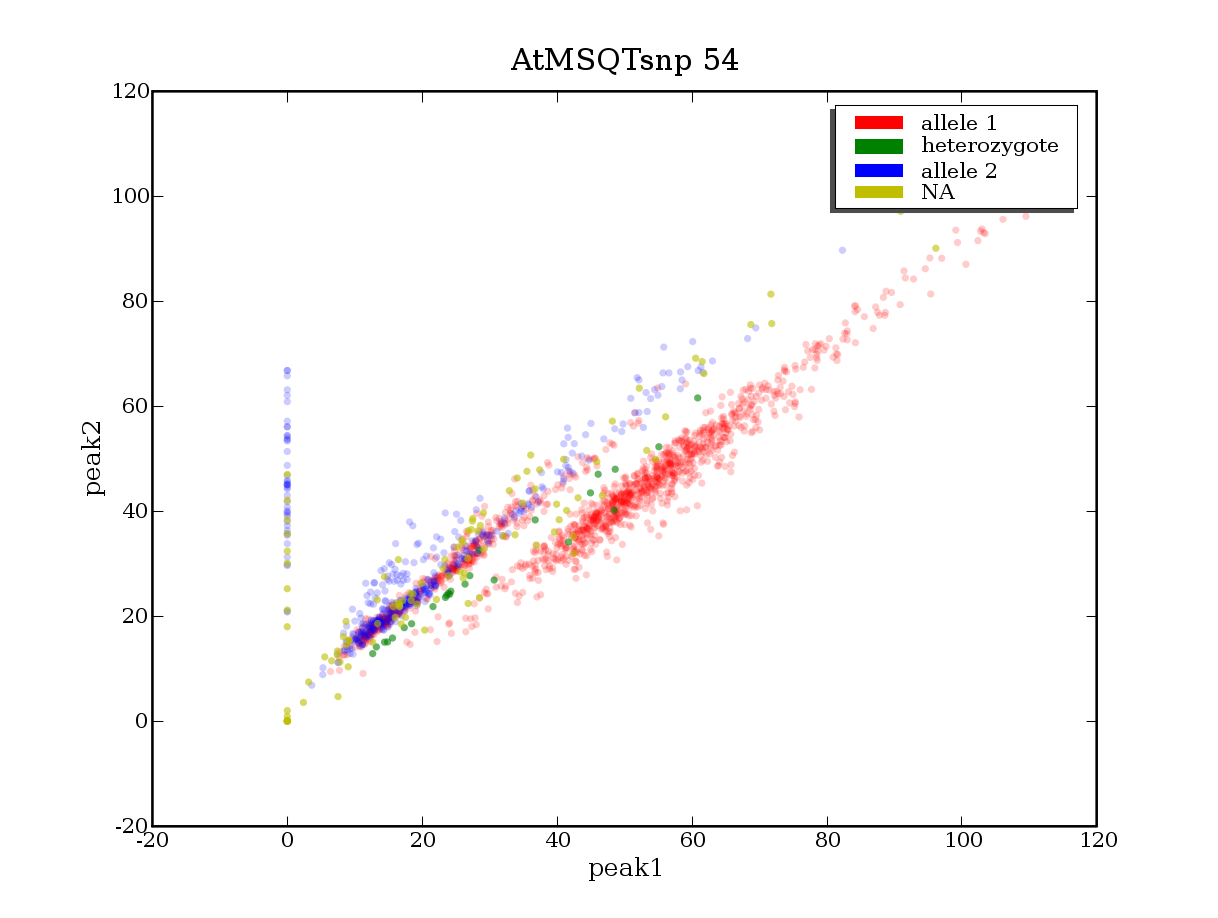
\includegraphics[width=0.5\textwidth]{figures/cluster_plot_AtMSQTsnp_54.png}
\caption{cluster plot for AtMSQTsnp 54.} \label{flAtMSQTsnp54}
\end{figure}
\begin{figure}[H]
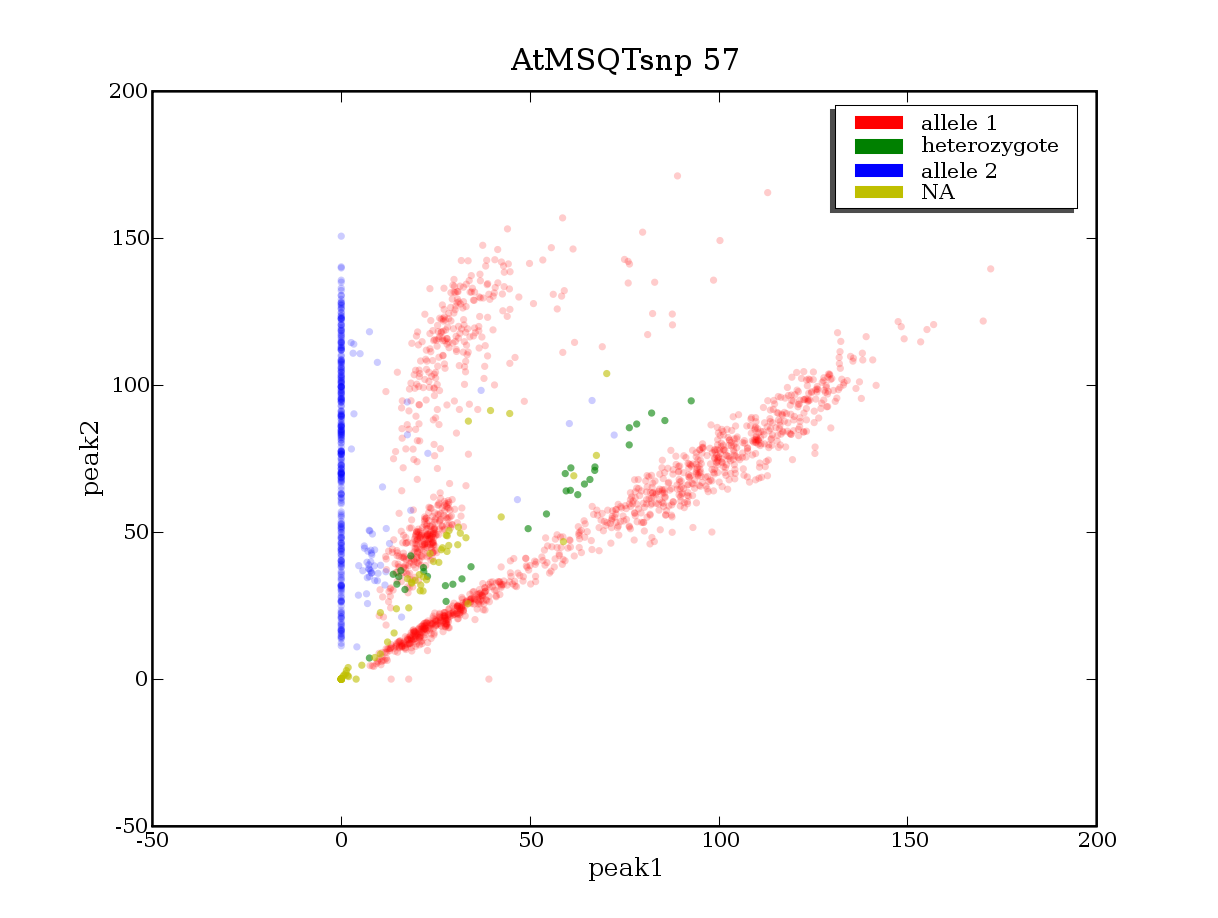
\includegraphics[width=0.5\textwidth]{figures/cluster_plot_AtMSQTsnp_57.png}
\caption{cluster plot for AtMSQTsnp 57.} \label{flAtMSQTsnp57}
\end{figure}
\begin{figure}[H]
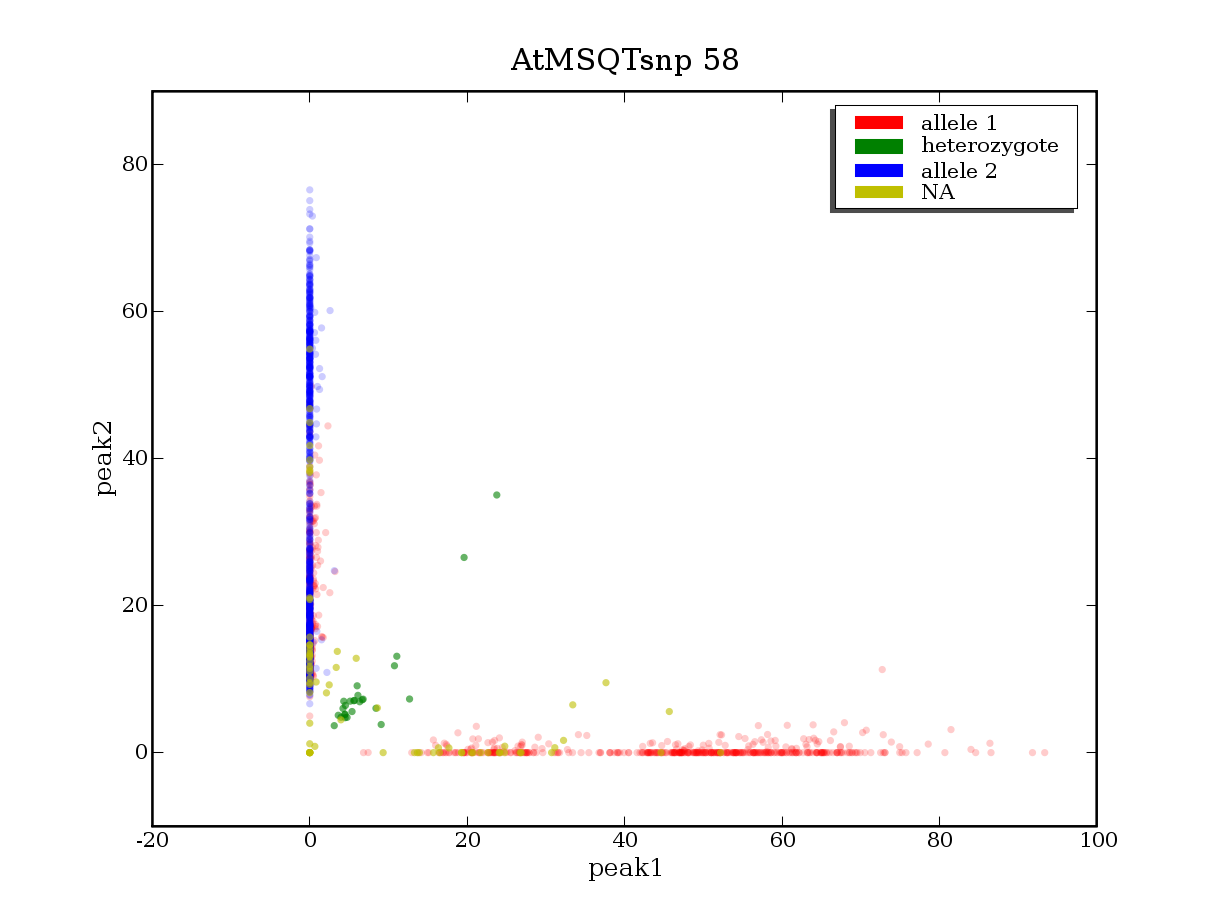
\includegraphics[width=0.5\textwidth]{figures/cluster_plot_AtMSQTsnp_58.png}
\caption{cluster plot for AtMSQTsnp 58.} \label{flAtMSQTsnp58}
\end{figure}
\begin{figure}[H]
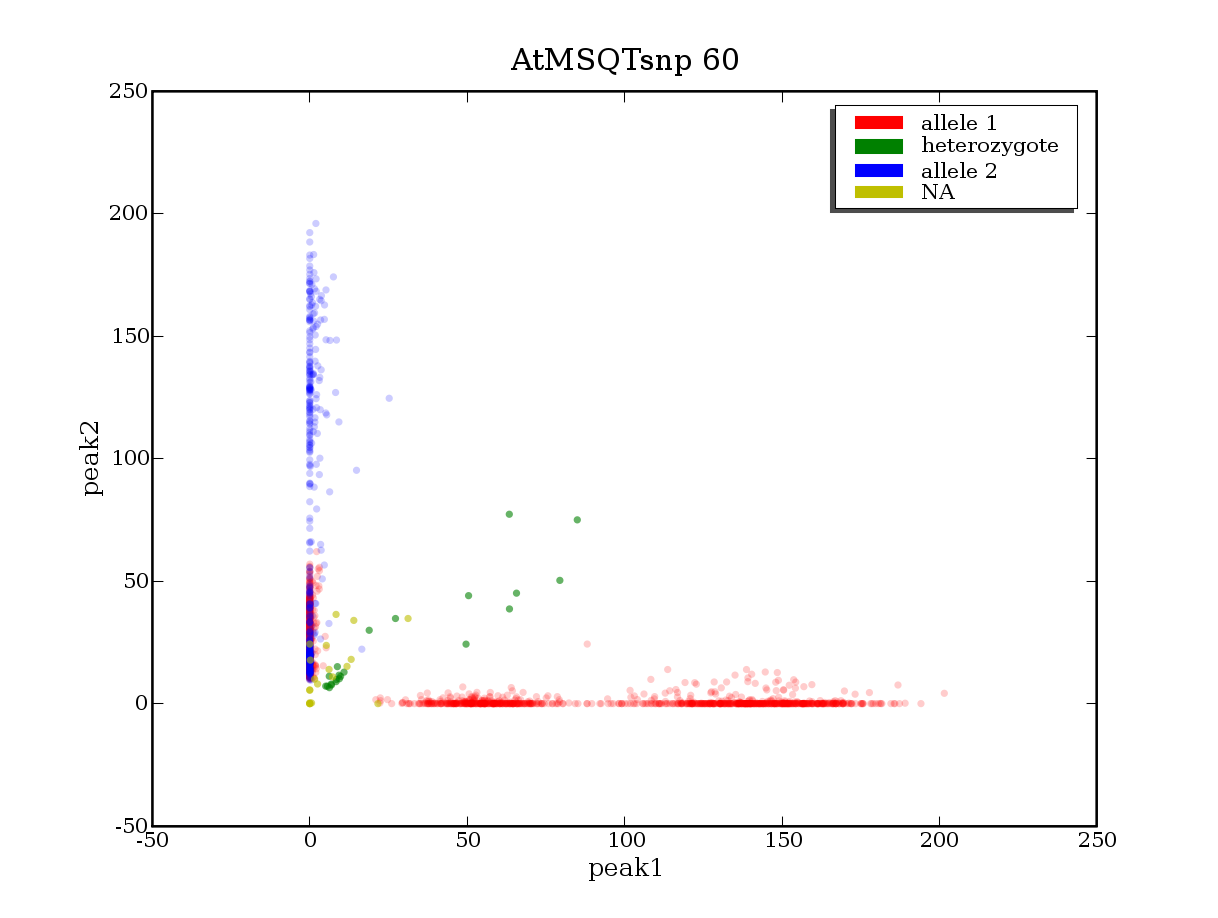
\includegraphics[width=0.5\textwidth]{figures/cluster_plot_AtMSQTsnp_60.png}
\caption{cluster plot for AtMSQTsnp 60.} \label{flAtMSQTsnp60}
\end{figure}
\begin{figure}[H]
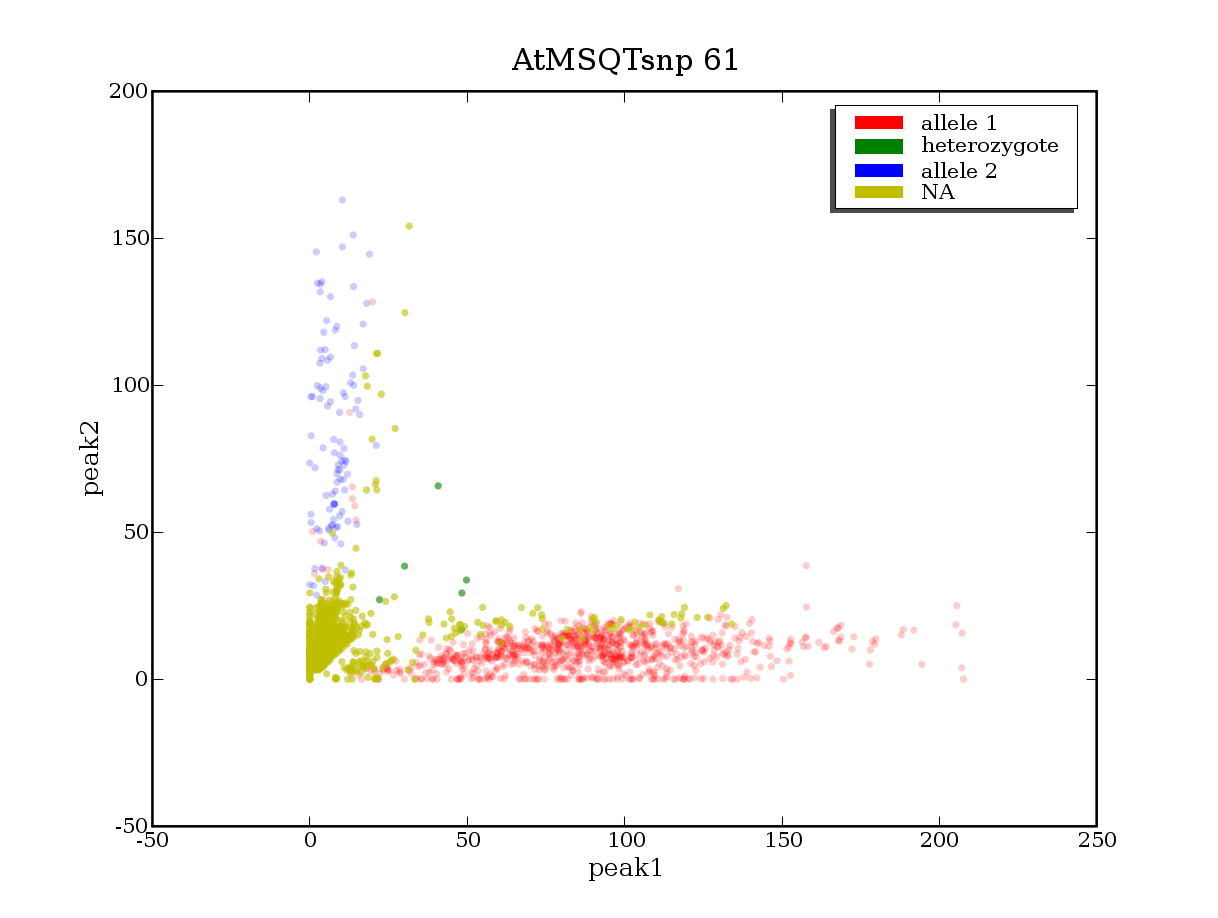
\includegraphics[width=0.5\textwidth]{figures/cluster_plot_AtMSQTsnp_61.png}
\caption{cluster plot for AtMSQTsnp 61.} \label{flAtMSQTsnp61}
\end{figure}
\begin{figure}[H]
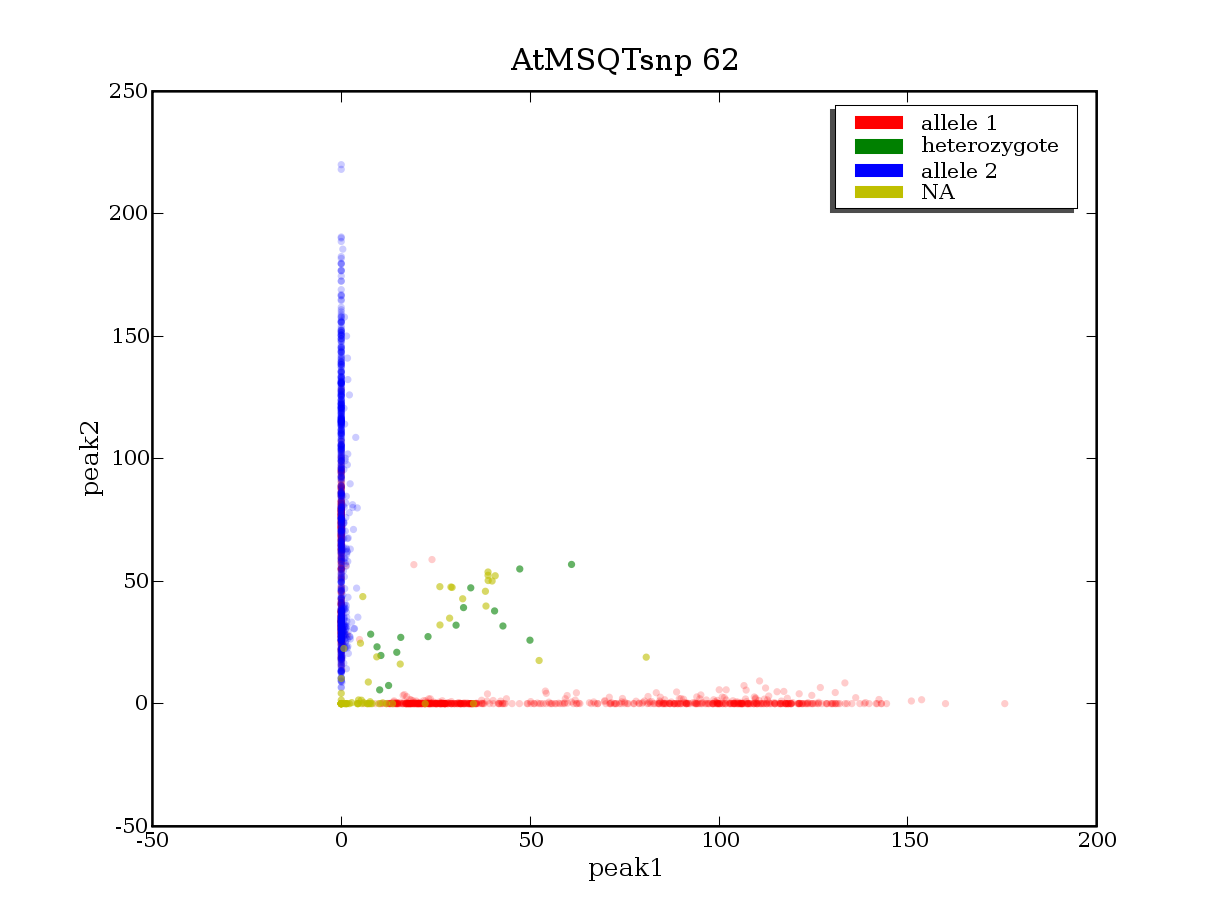
\includegraphics[width=0.5\textwidth]{figures/cluster_plot_AtMSQTsnp_62.png}
\caption{cluster plot for AtMSQTsnp 62.} \label{flAtMSQTsnp62}
\end{figure}
\begin{figure}[H]
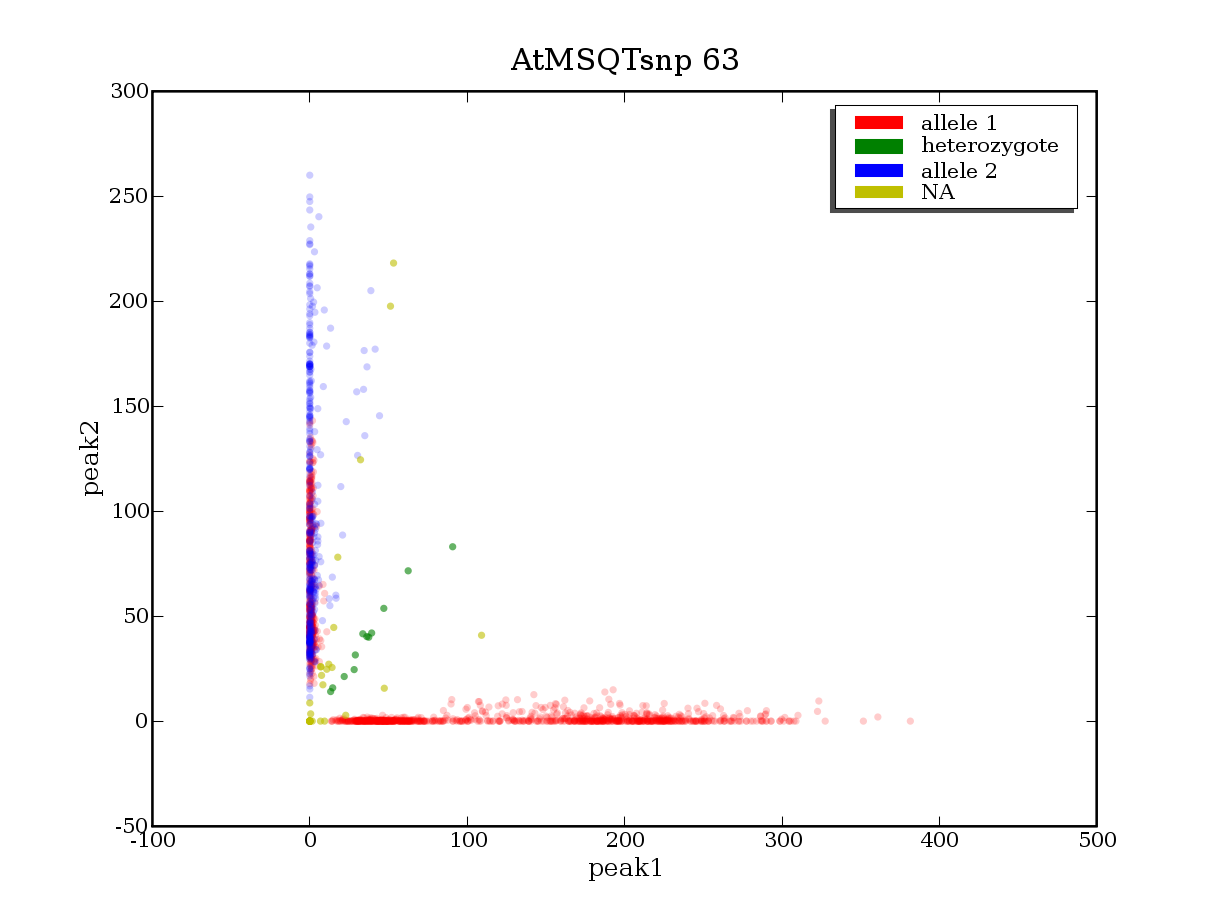
\includegraphics[width=0.5\textwidth]{figures/cluster_plot_AtMSQTsnp_63.png}
\caption{cluster plot for AtMSQTsnp 63.} \label{flAtMSQTsnp63}
\end{figure}
\begin{figure}[H]
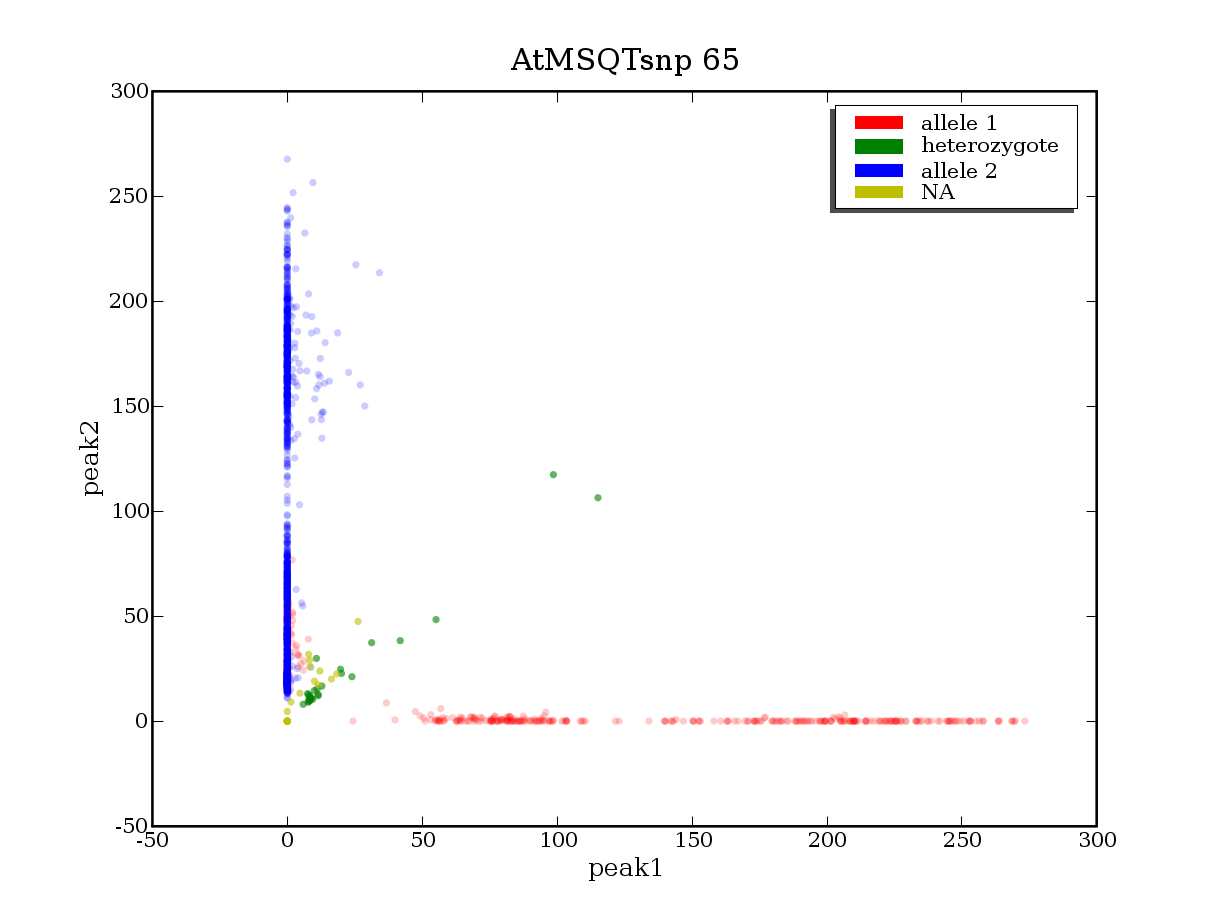
\includegraphics[width=0.5\textwidth]{figures/cluster_plot_AtMSQTsnp_65.png}
\caption{cluster plot for AtMSQTsnp 65.} \label{flAtMSQTsnp65}
\end{figure}
\begin{figure}[H]
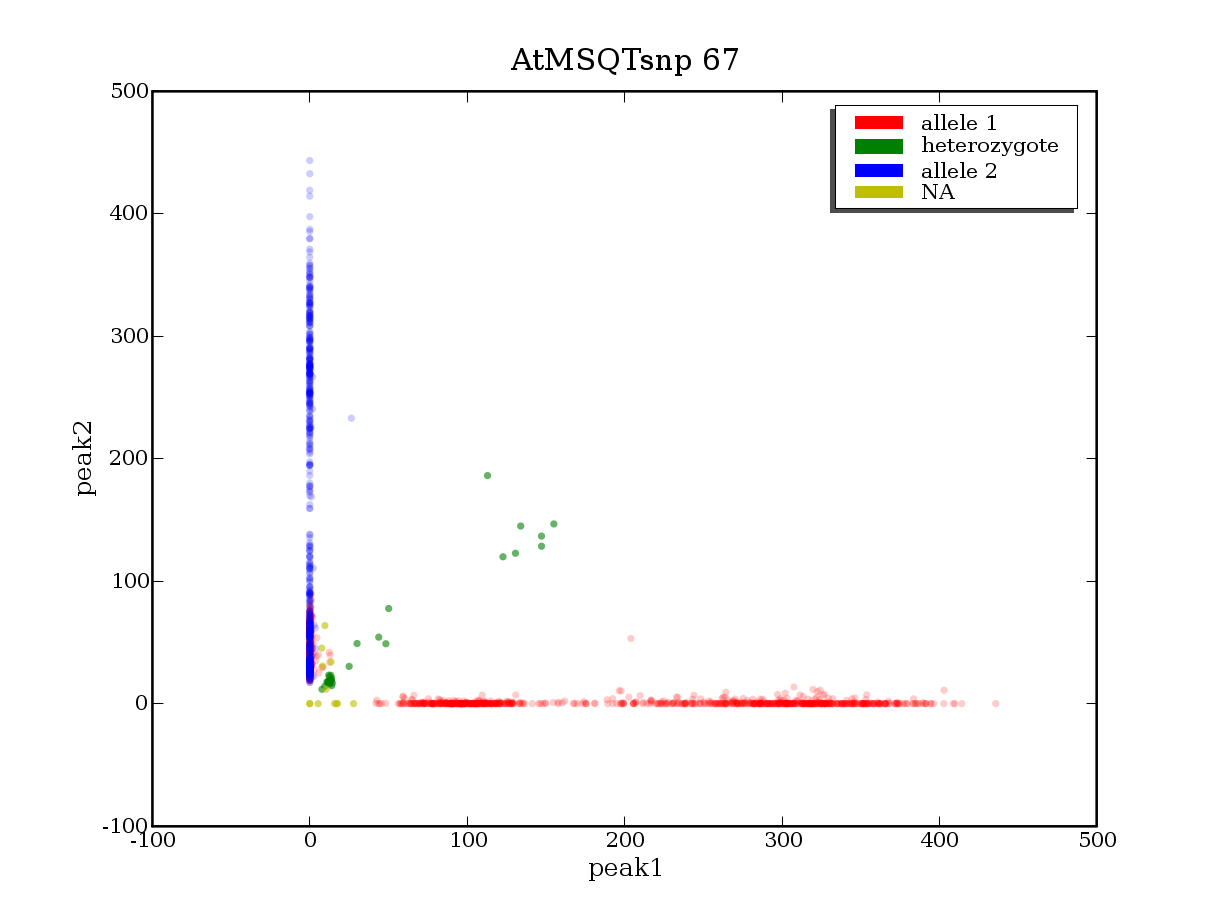
\includegraphics[width=0.5\textwidth]{figures/cluster_plot_AtMSQTsnp_67.png}
\caption{cluster plot for AtMSQTsnp 67.} \label{flAtMSQTsnp67}
\end{figure}
\begin{figure}[H]
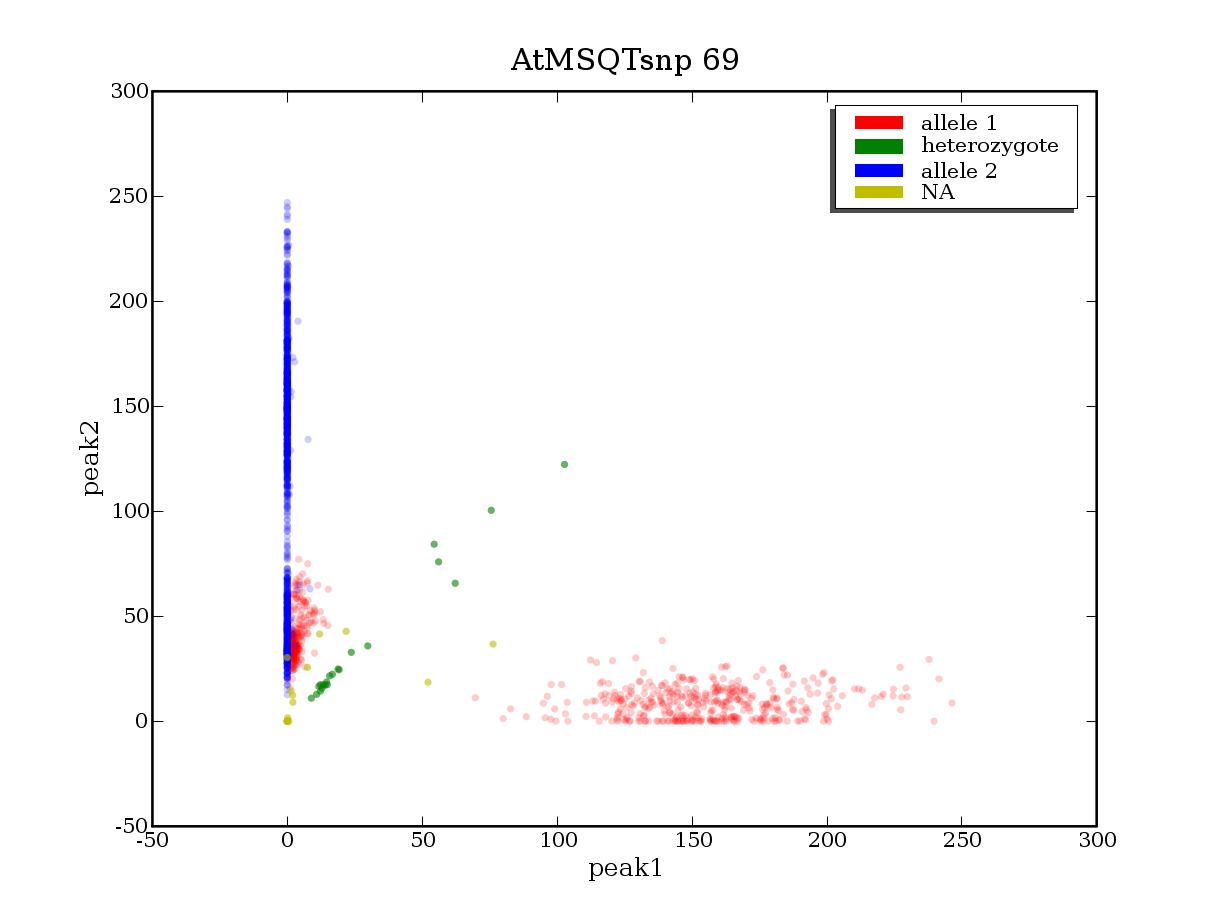
\includegraphics[width=0.5\textwidth]{figures/cluster_plot_AtMSQTsnp_69.png}
\caption{cluster plot for AtMSQTsnp 69.} \label{flAtMSQTsnp69}
\end{figure}
\begin{figure}[H]
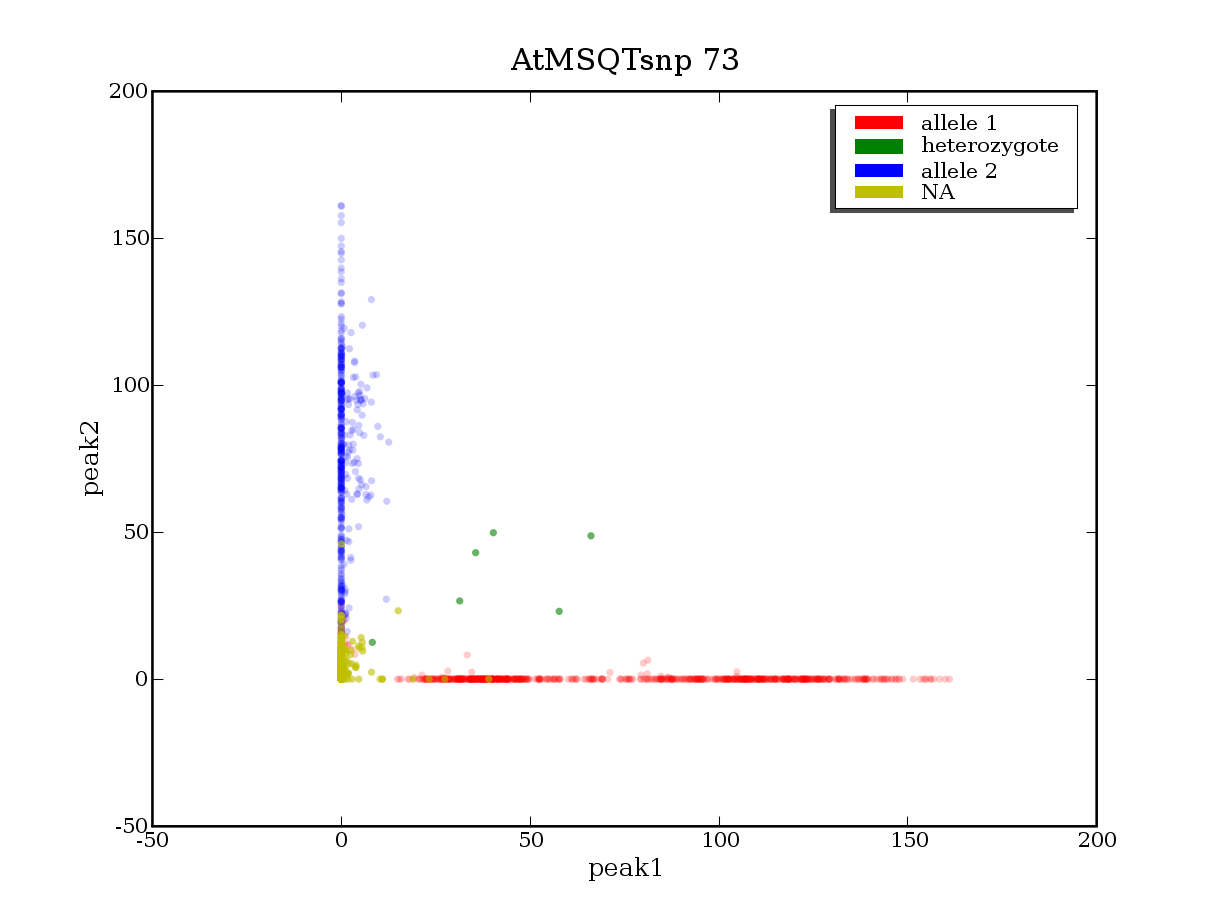
\includegraphics[width=0.5\textwidth]{figures/cluster_plot_AtMSQTsnp_73.png}
\caption{cluster plot for AtMSQTsnp 73.} \label{flAtMSQTsnp73}
\end{figure}
\begin{figure}[H]
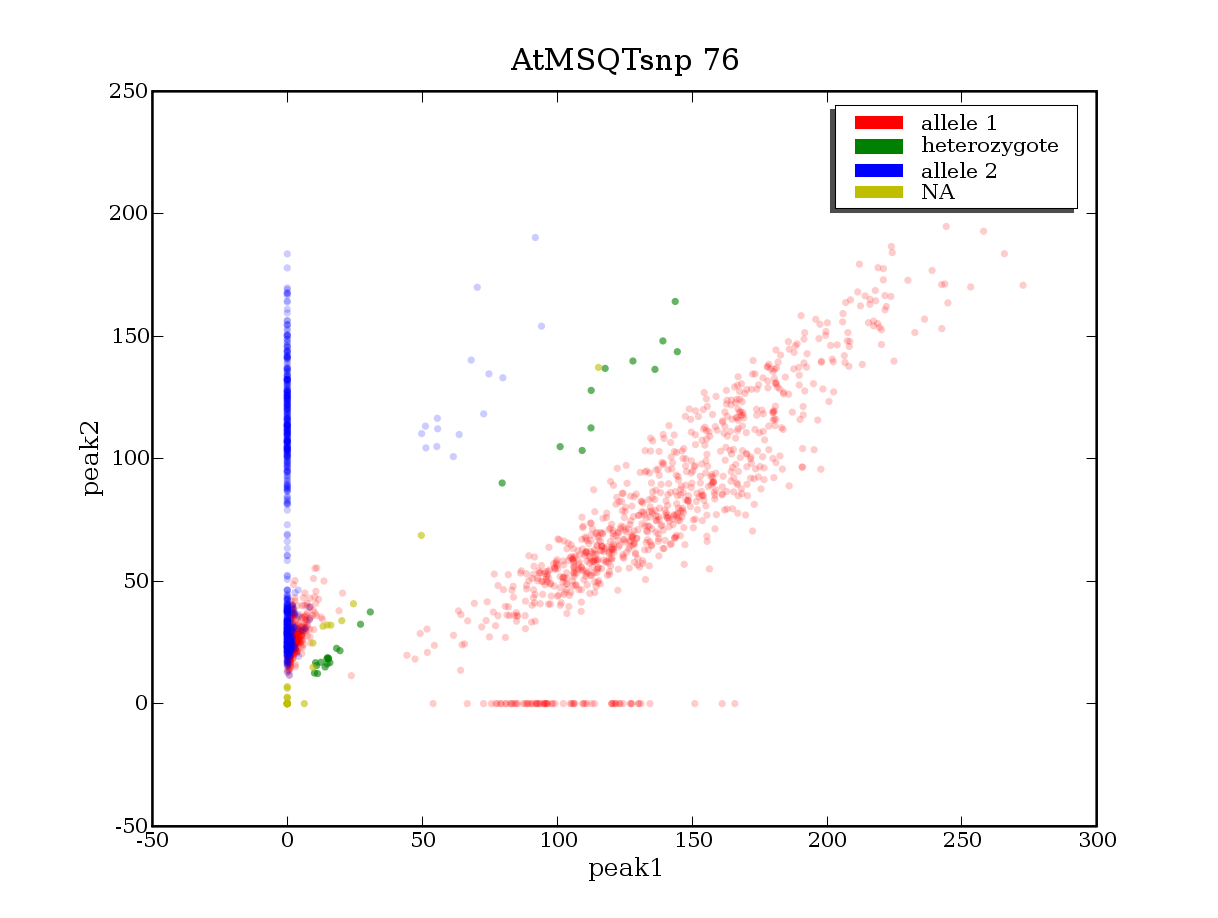
\includegraphics[width=0.5\textwidth]{figures/cluster_plot_AtMSQTsnp_76.png}
\caption{cluster plot for AtMSQTsnp 76.} \label{flAtMSQTsnp76}
\end{figure}
\begin{figure}[H]
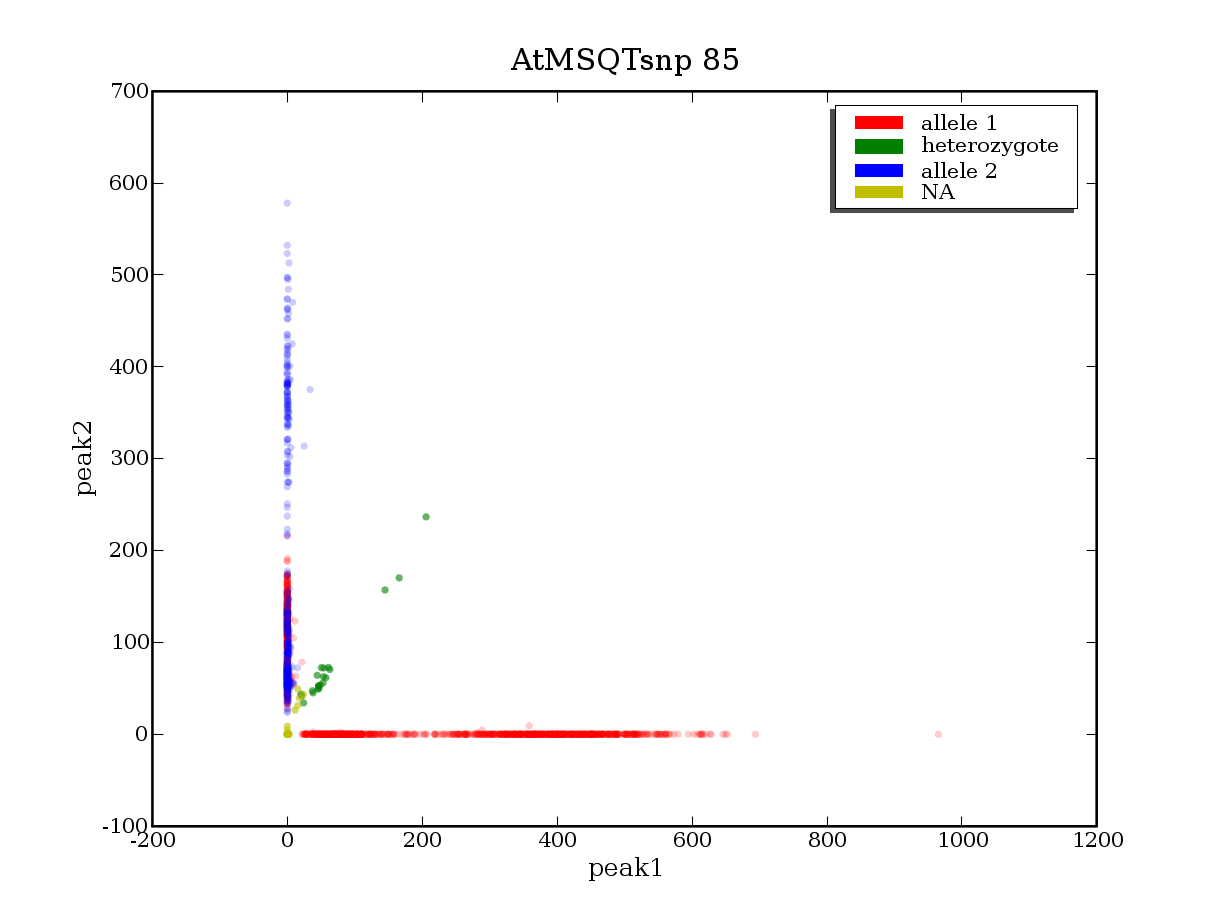
\includegraphics[width=0.5\textwidth]{figures/cluster_plot_AtMSQTsnp_85.png}
\caption{cluster plot for AtMSQTsnp 85.} \label{flAtMSQTsnp85}
\end{figure}
\begin{figure}[H]
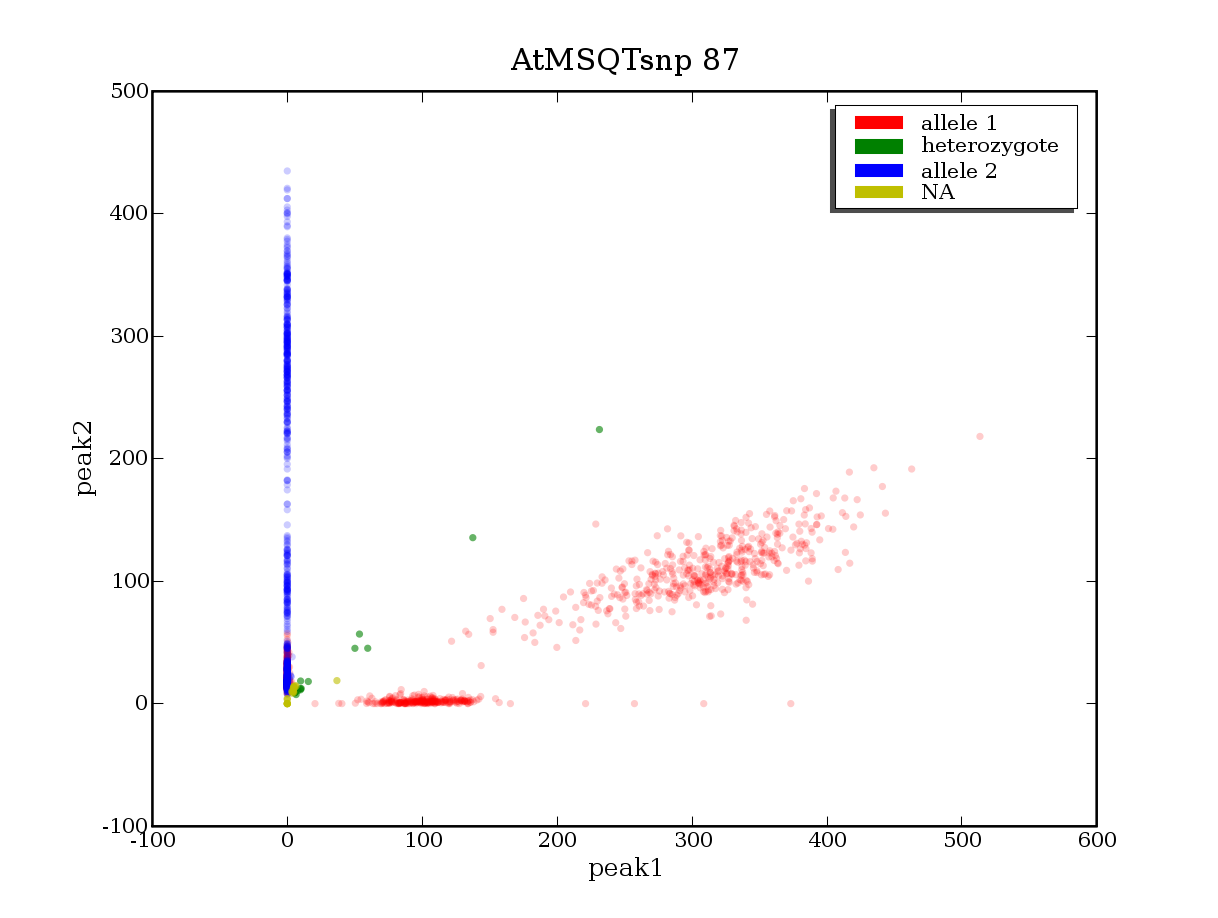
\includegraphics[width=0.5\textwidth]{figures/cluster_plot_AtMSQTsnp_87.png}
\caption{cluster plot for AtMSQTsnp 87.} \label{flAtMSQTsnp87}
\end{figure}
\begin{figure}[H]
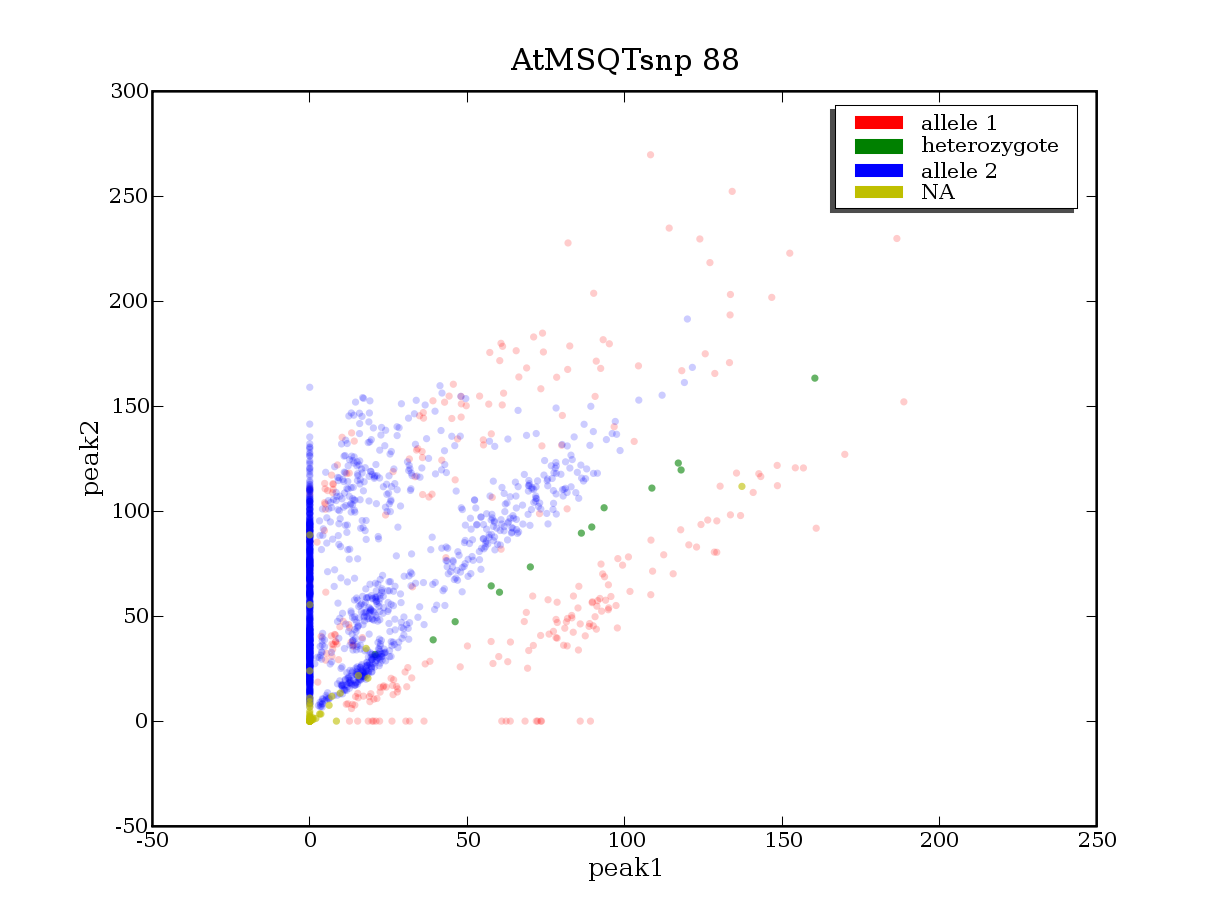
\includegraphics[width=0.5\textwidth]{figures/cluster_plot_AtMSQTsnp_88.png}
\caption{cluster plot for AtMSQTsnp 88.} \label{flAtMSQTsnp88}
\end{figure}
\begin{figure}[H]
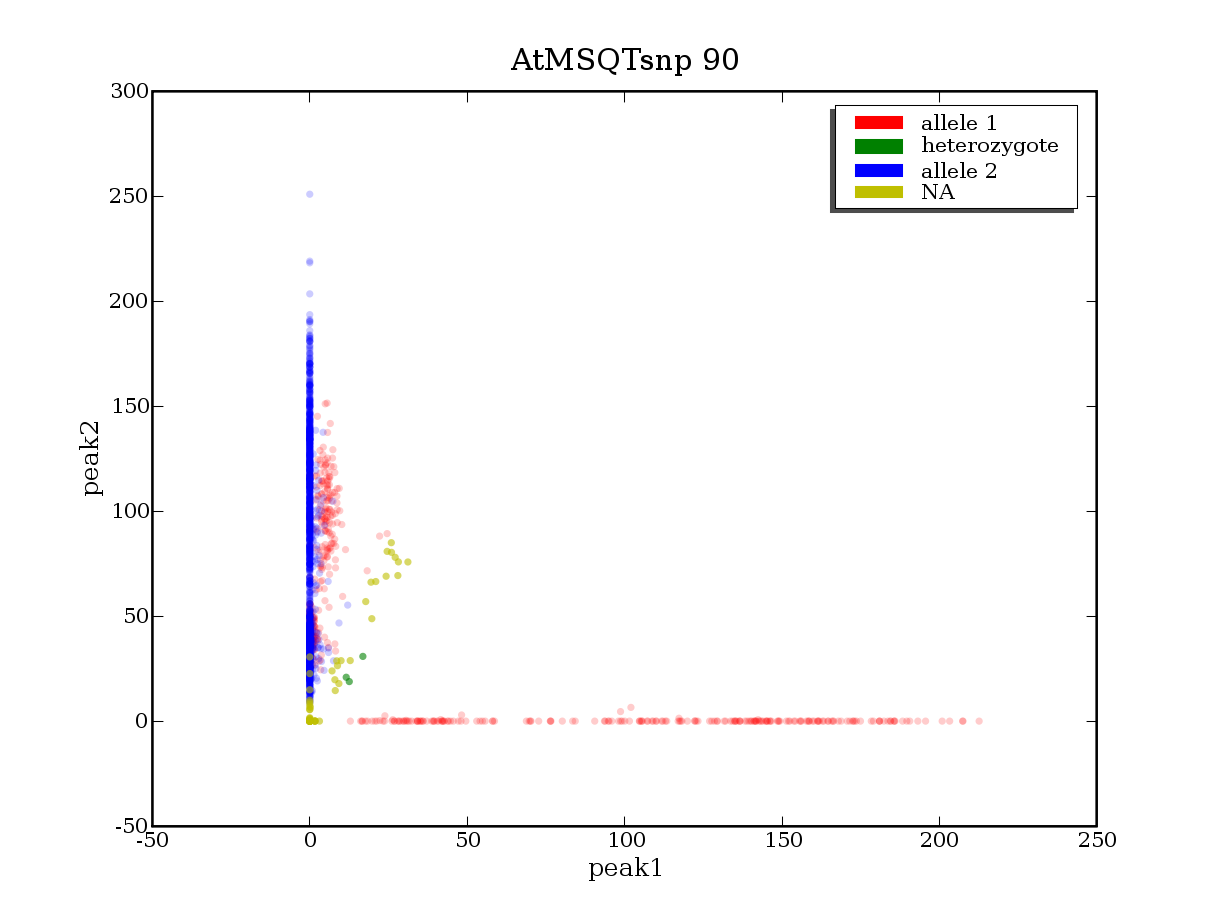
\includegraphics[width=0.5\textwidth]{figures/cluster_plot_AtMSQTsnp_90.png}
\caption{cluster plot for AtMSQTsnp 90.} \label{flAtMSQTsnp90}
\end{figure}
\begin{figure}[H]
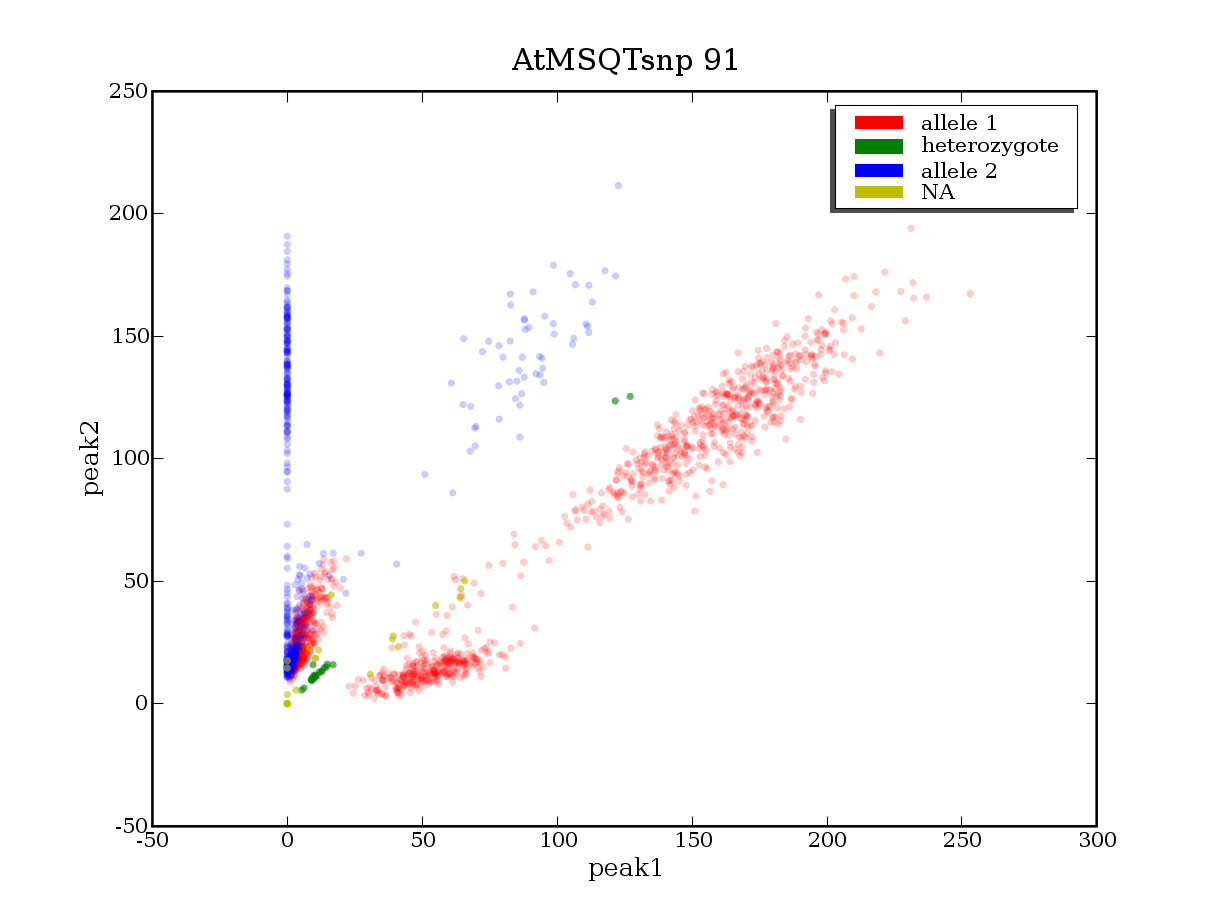
\includegraphics[width=0.5\textwidth]{figures/cluster_plot_AtMSQTsnp_91.png}
\caption{cluster plot for AtMSQTsnp 91.} \label{flAtMSQTsnp91}
\end{figure}
\begin{figure}[H]
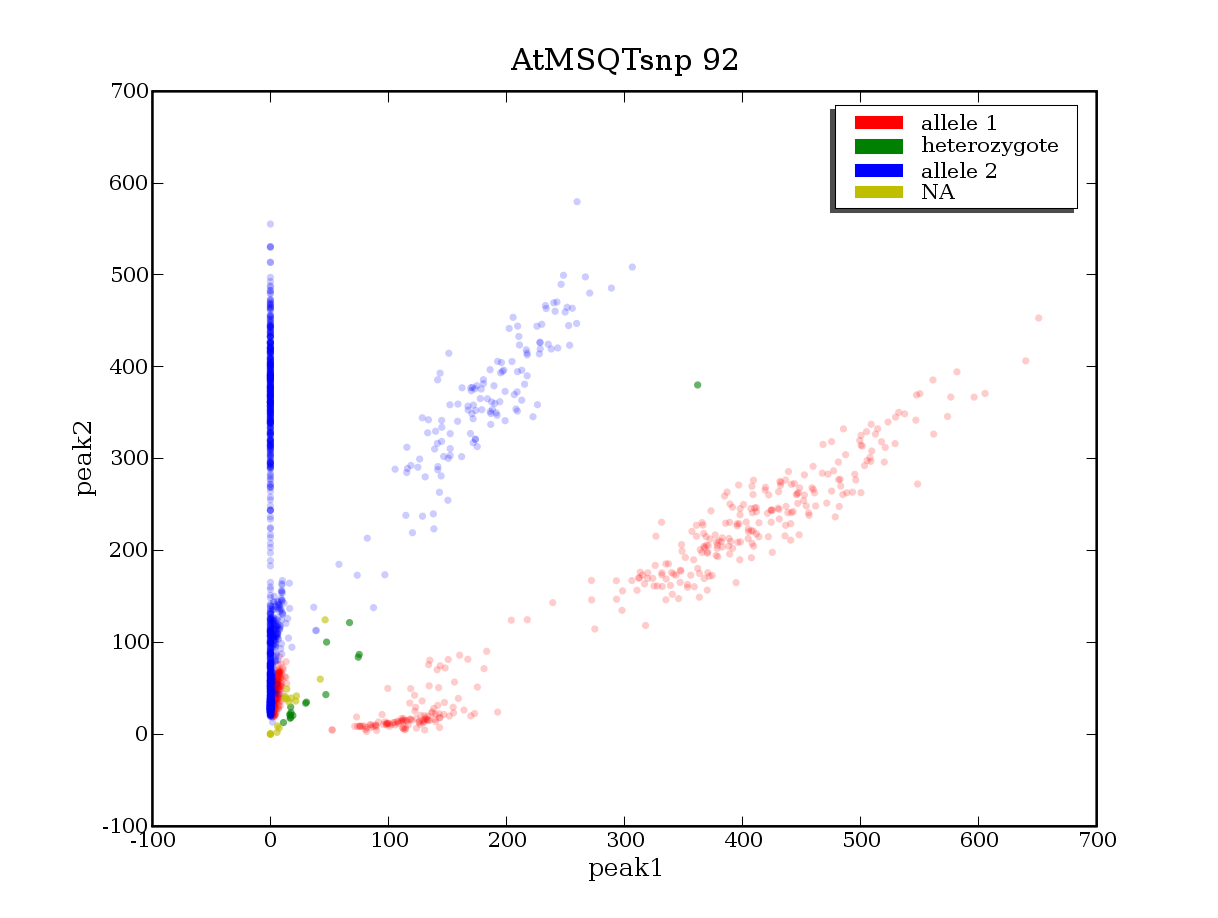
\includegraphics[width=0.5\textwidth]{figures/cluster_plot_AtMSQTsnp_92.png}
\caption{cluster plot for AtMSQTsnp 92.} \label{flAtMSQTsnp92}
\end{figure}
\begin{figure}[H]
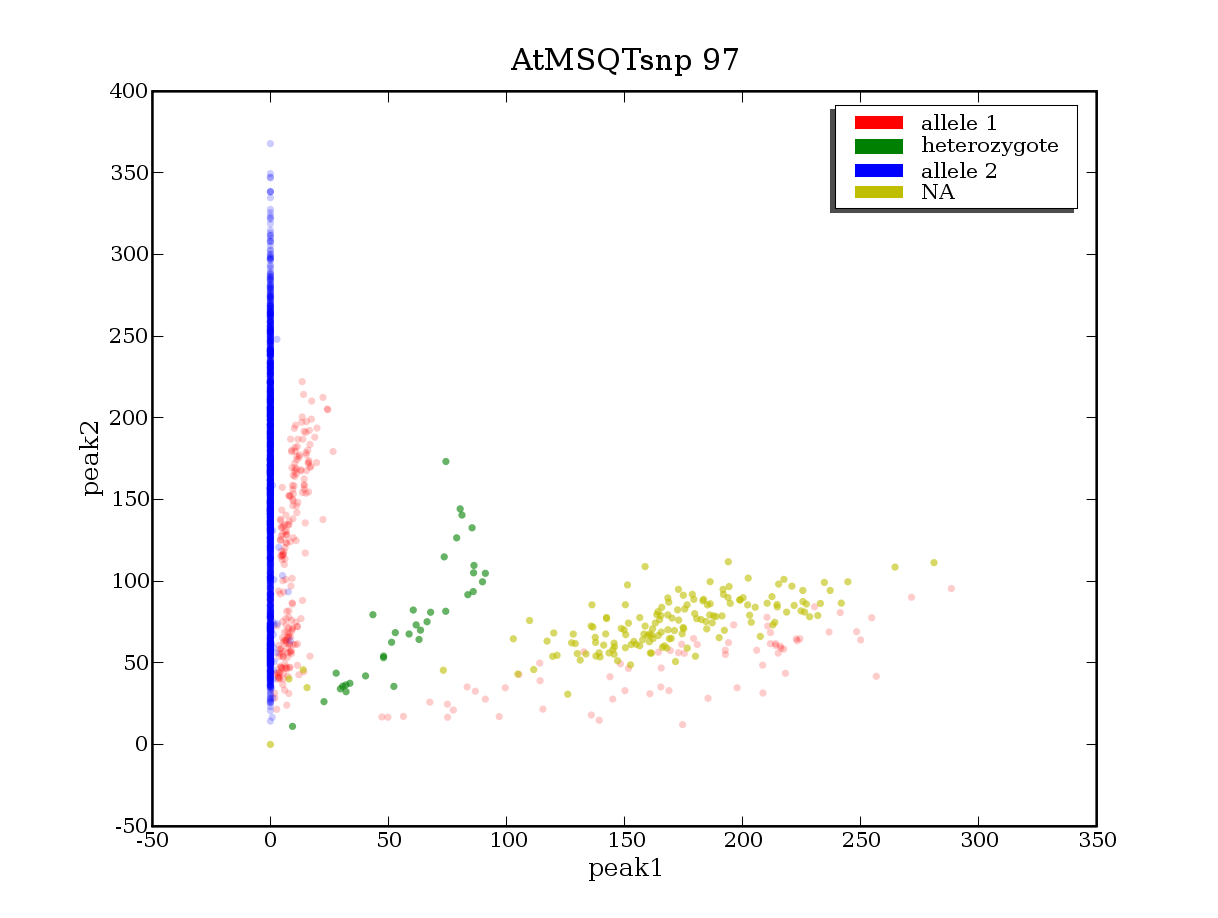
\includegraphics[width=0.5\textwidth]{figures/cluster_plot_AtMSQTsnp_97.png}
\caption{cluster plot for AtMSQTsnp 97.} \label{flAtMSQTsnp97}
\end{figure}
\begin{figure}[H]
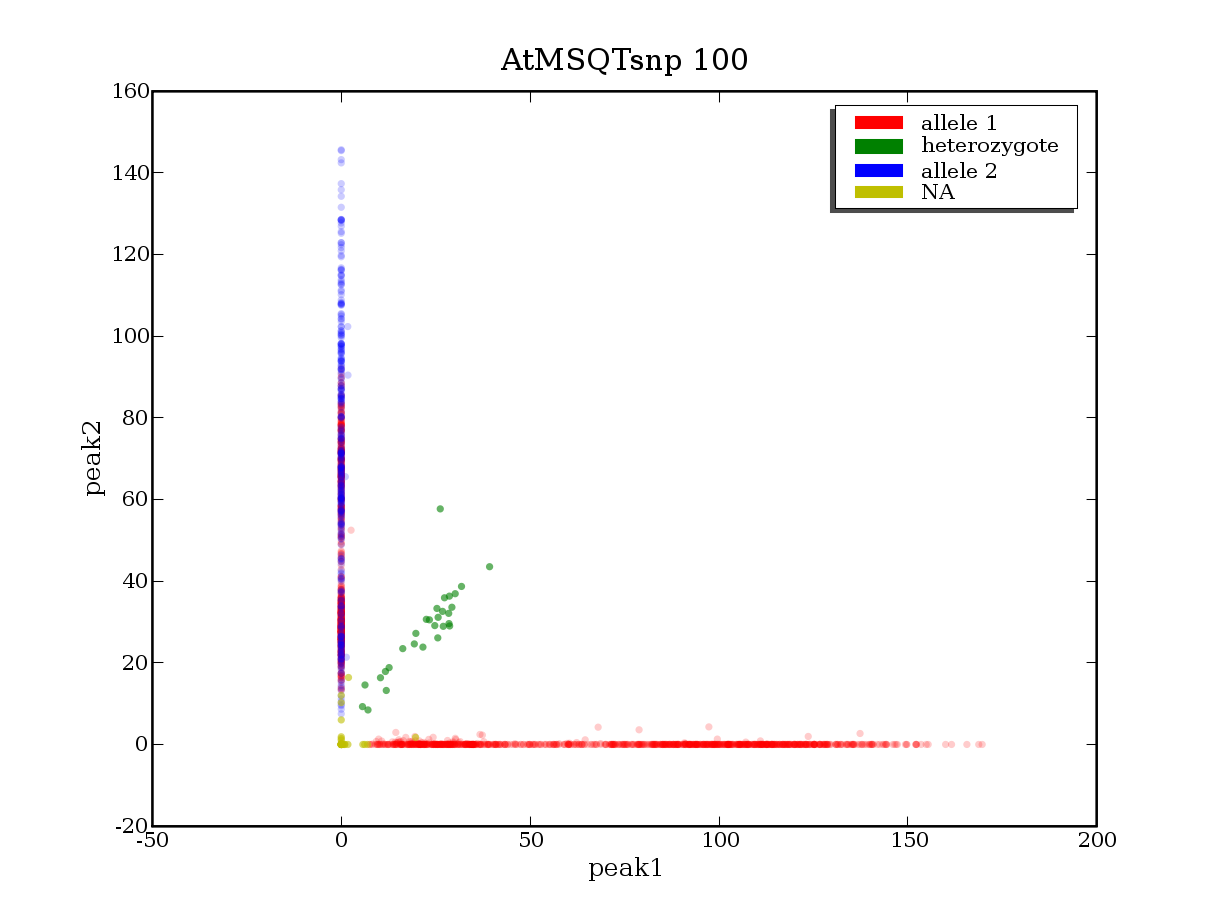
\includegraphics[width=0.5\textwidth]{figures/cluster_plot_AtMSQTsnp_100.png}
\caption{cluster plot for AtMSQTsnp 100.} \label{flAtMSQTsnp100}
\end{figure}
\begin{figure}[H]
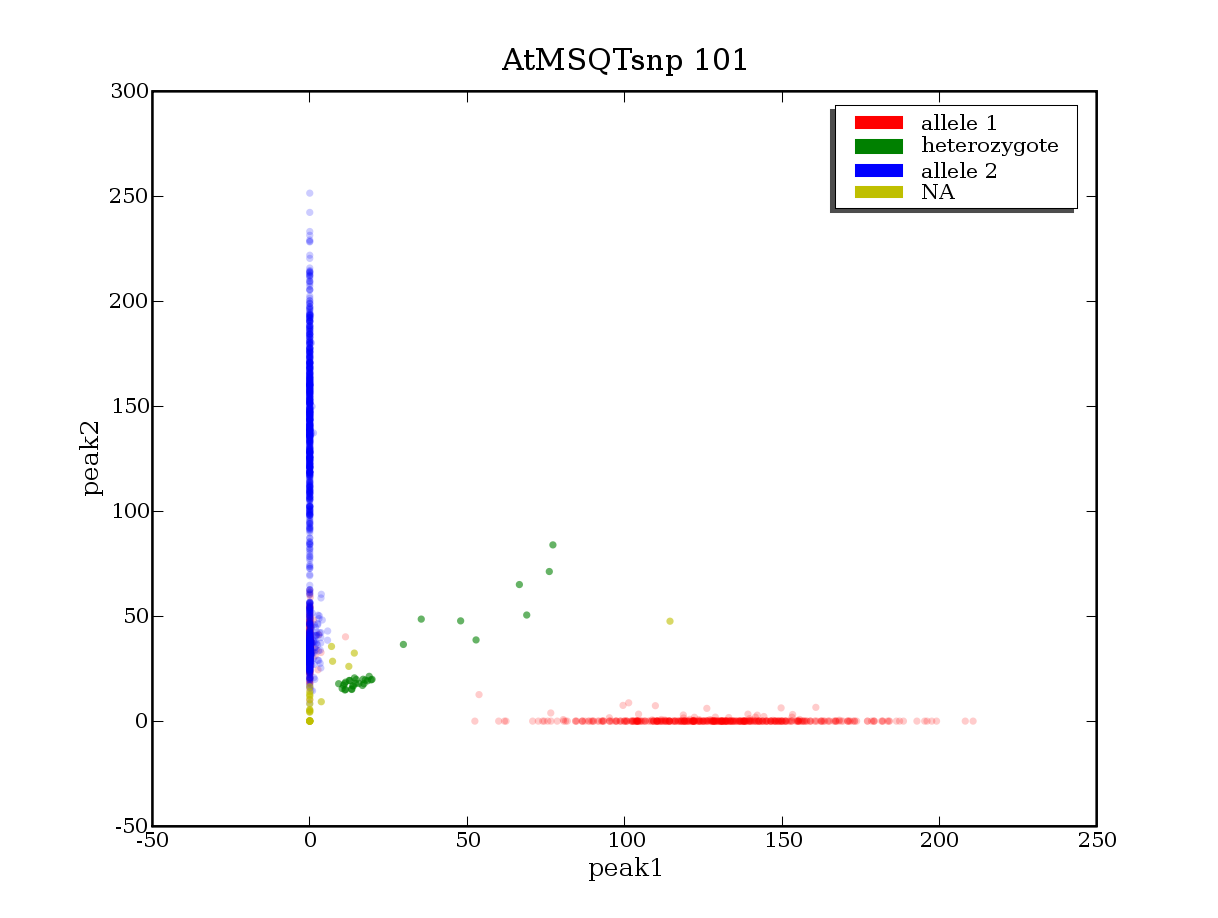
\includegraphics[width=0.5\textwidth]{figures/cluster_plot_AtMSQTsnp_101.png}
\caption{cluster plot for AtMSQTsnp 101.} \label{flAtMSQTsnp101}
\end{figure}
\begin{figure}[H]
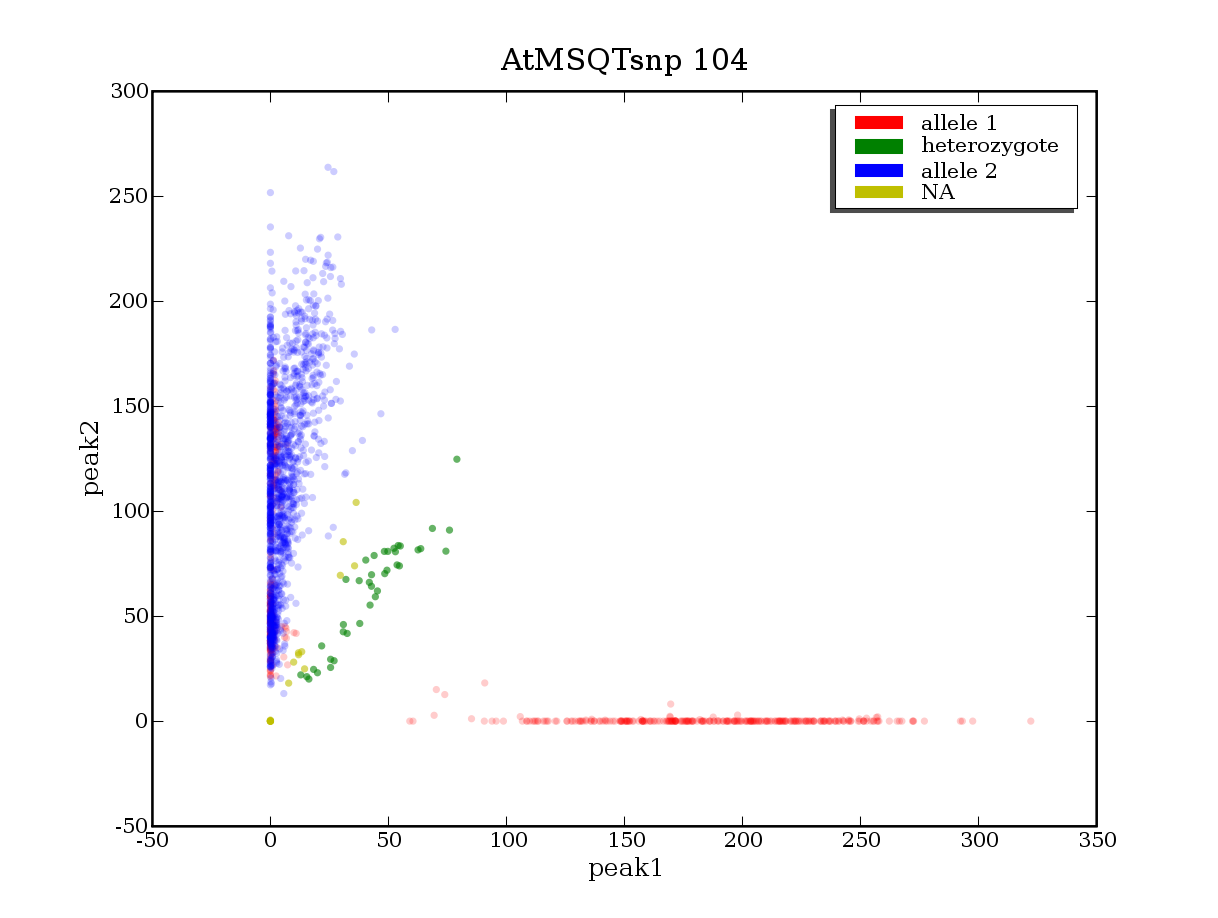
\includegraphics[width=0.5\textwidth]{figures/cluster_plot_AtMSQTsnp_104.png}
\caption{cluster plot for AtMSQTsnp 104.} \label{flAtMSQTsnp104}
\end{figure}
\begin{figure}[H]
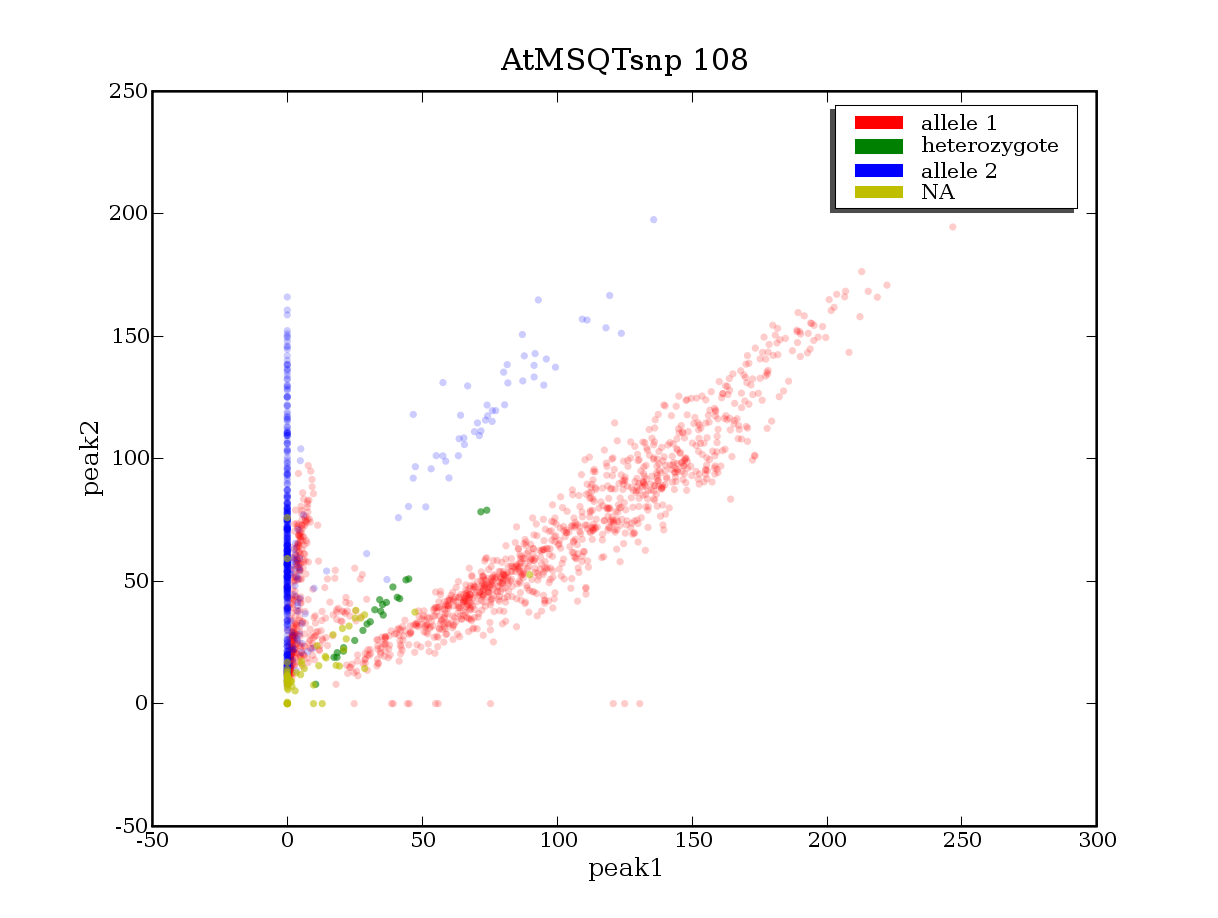
\includegraphics[width=0.5\textwidth]{figures/cluster_plot_AtMSQTsnp_108.png}
\caption{cluster plot for AtMSQTsnp 108.} \label{flAtMSQTsnp108}
\end{figure}
\begin{figure}[H]
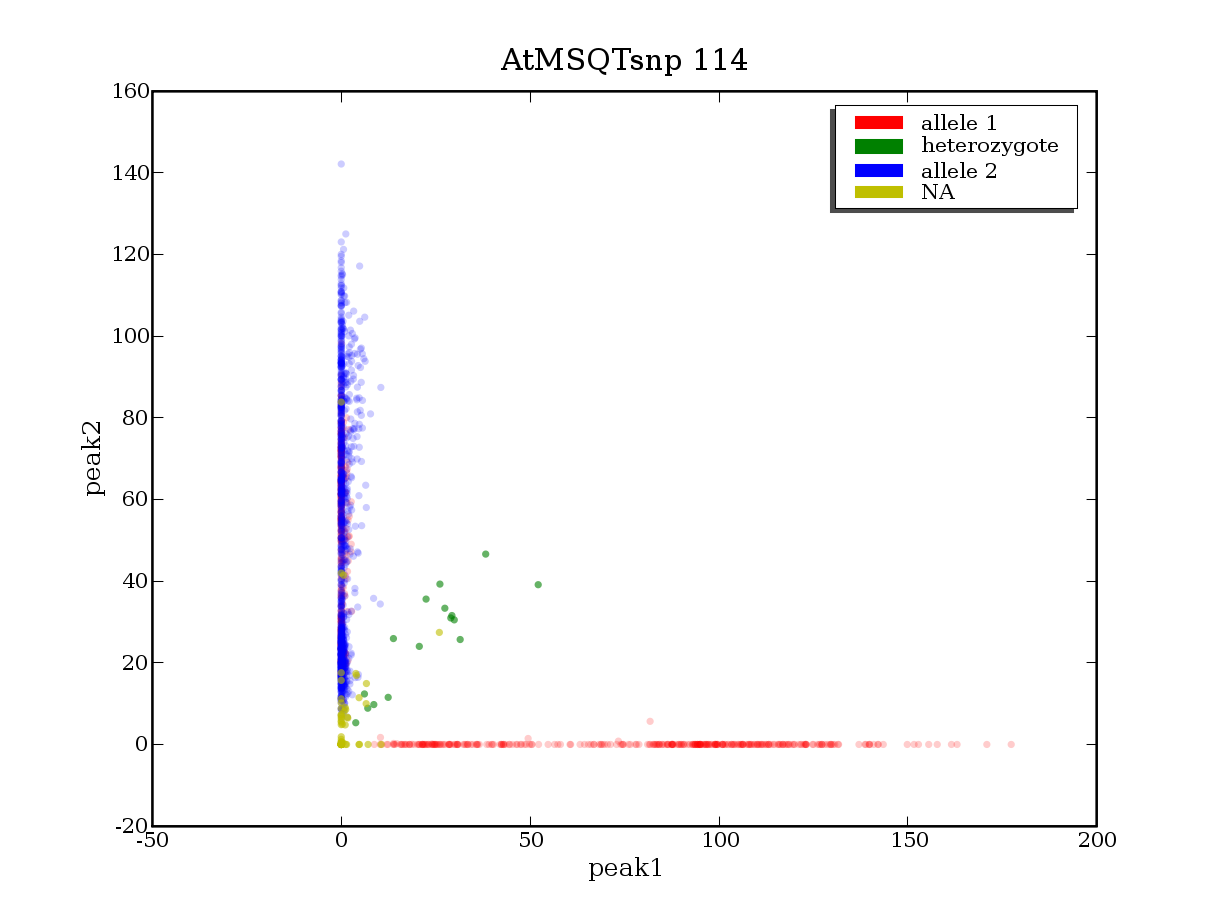
\includegraphics[width=0.5\textwidth]{figures/cluster_plot_AtMSQTsnp_114.png}
\caption{cluster plot for AtMSQTsnp 114.} \label{flAtMSQTsnp114}
\end{figure}
\begin{figure}[H]
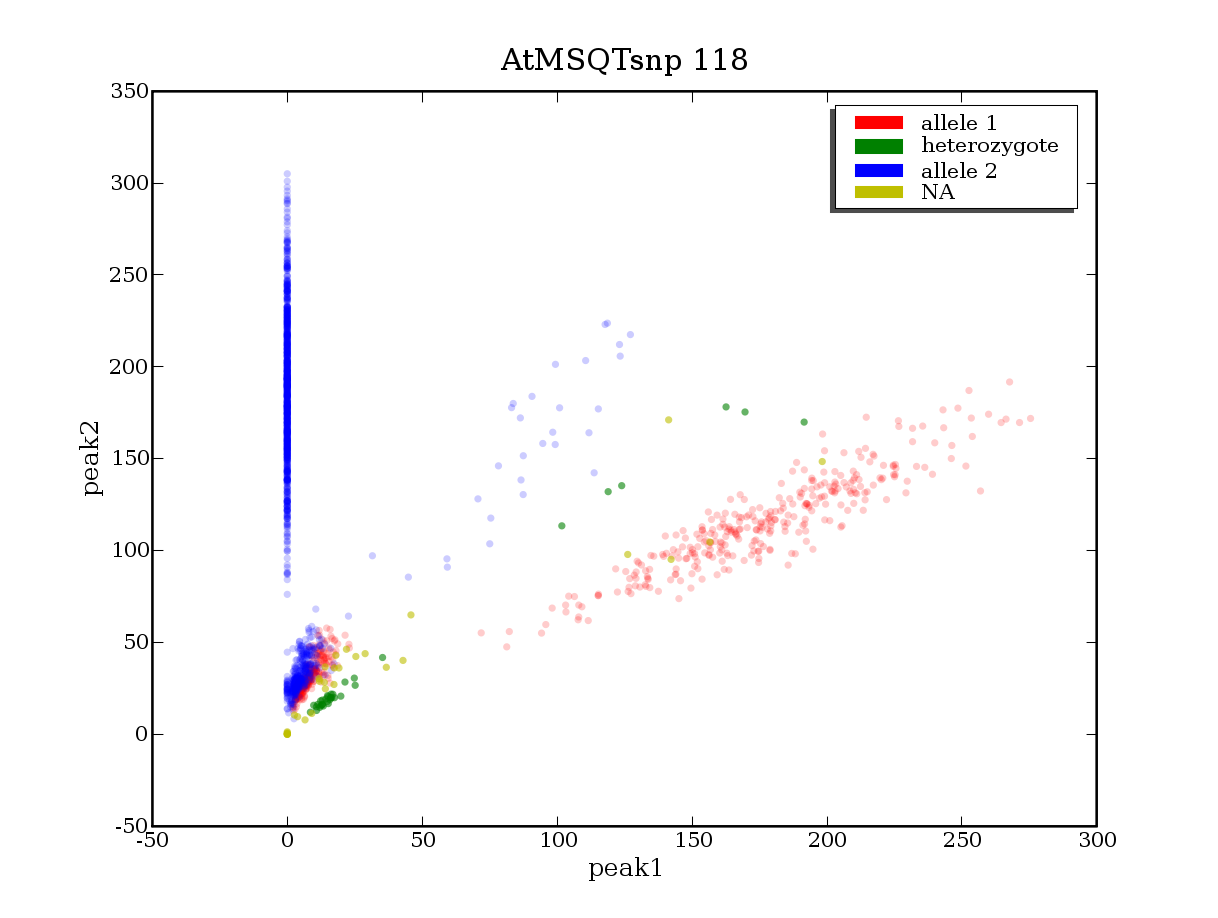
\includegraphics[width=0.5\textwidth]{figures/cluster_plot_AtMSQTsnp_118.png}
\caption{cluster plot for AtMSQTsnp 118.} \label{flAtMSQTsnp118}
\end{figure}
\begin{figure}[H]
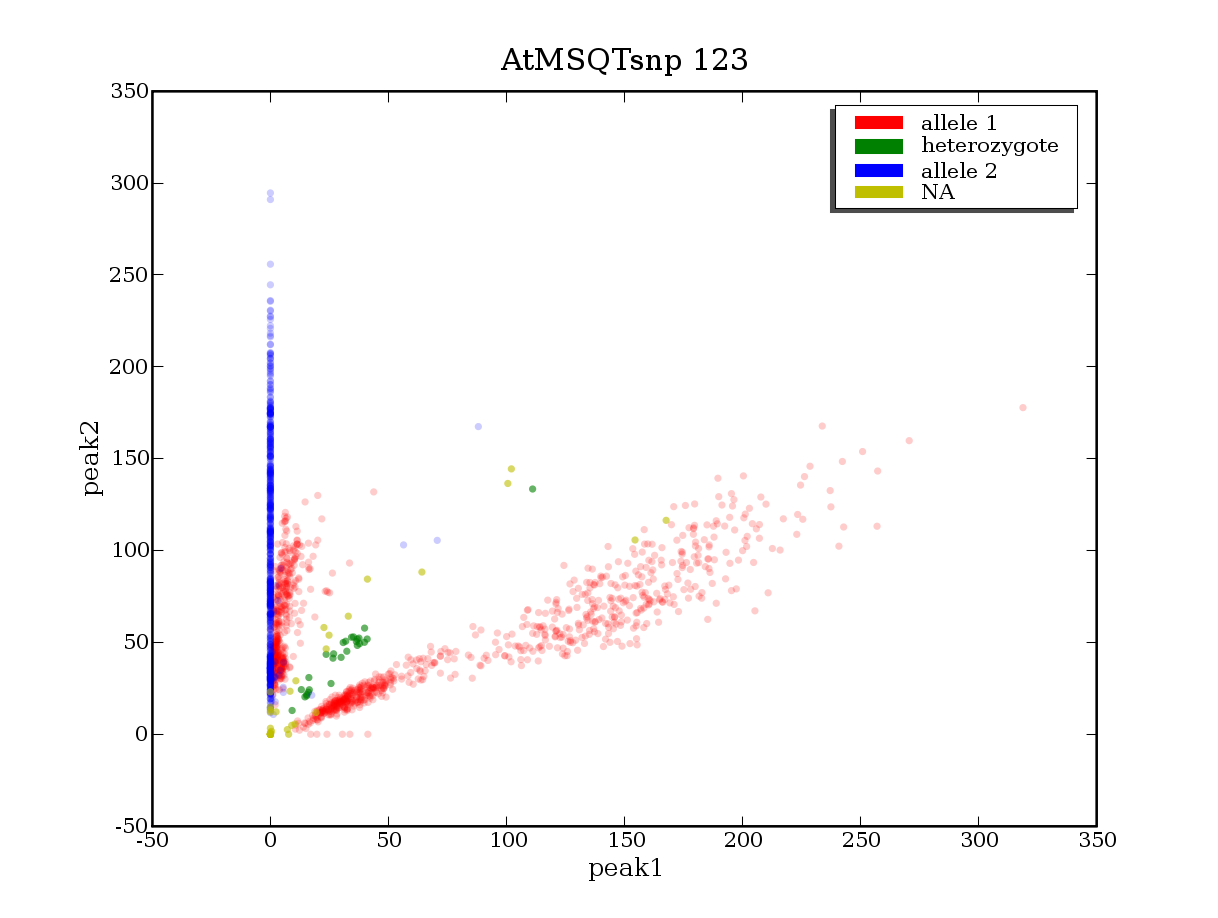
\includegraphics[width=0.5\textwidth]{figures/cluster_plot_AtMSQTsnp_123.png}
\caption{cluster plot for AtMSQTsnp 123.} \label{flAtMSQTsnp123}
\end{figure}
\begin{figure}[H]
\includegraphics[width=0.5\textwidth]{figures/cluster_plot_AtMSQTsnp_126.png}
\caption{cluster plot for AtMSQTsnp 126.} \label{flAtMSQTsnp126}
\end{figure}
\begin{figure}[H]
\includegraphics[width=0.5\textwidth]{figures/cluster_plot_AtMSQTsnp_128.png}
\caption{cluster plot for AtMSQTsnp 128.} \label{flAtMSQTsnp128}
\end{figure}
\begin{figure}[H]
\includegraphics[width=0.5\textwidth]{figures/cluster_plot_AtMSQTsnp_129.png}
\caption{cluster plot for AtMSQTsnp 129.} \label{flAtMSQTsnp129}
\end{figure}
\begin{figure}[H]
\includegraphics[width=0.5\textwidth]{figures/cluster_plot_AtMSQTsnp_130.png}
\caption{cluster plot for AtMSQTsnp 130.} \label{flAtMSQTsnp130}
\end{figure}
\begin{figure}[H]
\includegraphics[width=0.5\textwidth]{figures/cluster_plot_AtMSQTsnp_132.png}
\caption{cluster plot for AtMSQTsnp 132.} \label{flAtMSQTsnp132}
\end{figure}
\begin{figure}[H]
\includegraphics[width=0.5\textwidth]{figures/cluster_plot_AtMSQTsnp_138.png}
\caption{cluster plot for AtMSQTsnp 138.} \label{flAtMSQTsnp138}
\end{figure}
\begin{figure}[H]
\includegraphics[width=0.5\textwidth]{figures/cluster_plot_AtMSQTsnp_140.png}
\caption{cluster plot for AtMSQTsnp 140.} \label{flAtMSQTsnp140}
\end{figure}
\begin{figure}[H]
\includegraphics[width=0.5\textwidth]{figures/cluster_plot_AtMSQTsnp_142.png}
\caption{cluster plot for AtMSQTsnp 142.} \label{flAtMSQTsnp142}
\end{figure}
\begin{figure}[H]
\includegraphics[width=0.5\textwidth]{figures/cluster_plot_AtMSQTsnp_143.png}
\caption{cluster plot for AtMSQTsnp 143.} \label{flAtMSQTsnp143}
\end{figure}
\begin{figure}[H]
\includegraphics[width=0.5\textwidth]{figures/cluster_plot_AtMSQTsnp_145.png}
\caption{cluster plot for AtMSQTsnp 145.} \label{flAtMSQTsnp145}
\end{figure}
\begin{figure}[H]
\includegraphics[width=0.5\textwidth]{figures/cluster_plot_AtMSQTsnp_146.png}
\caption{cluster plot for AtMSQTsnp 146.} \label{flAtMSQTsnp146}
\end{figure}
\begin{figure}[H]
\includegraphics[width=0.5\textwidth]{figures/cluster_plot_AtMSQTsnp_155.png}
\caption{cluster plot for AtMSQTsnp 155.} \label{flAtMSQTsnp155}
\end{figure}
\begin{figure}[H]
\includegraphics[width=0.5\textwidth]{figures/cluster_plot_AtMSQTsnp_156.png}
\caption{cluster plot for AtMSQTsnp 156.} \label{flAtMSQTsnp156}
\end{figure}
\begin{figure}[H]
\includegraphics[width=0.5\textwidth]{figures/cluster_plot_AtMSQTsnp_159.png}
\caption{cluster plot for AtMSQTsnp 159.} \label{flAtMSQTsnp159}
\end{figure}
\begin{figure}[H]
\includegraphics[width=0.5\textwidth]{figures/cluster_plot_AtMSQTsnp_164.png}
\caption{cluster plot for AtMSQTsnp 164.} \label{flAtMSQTsnp164}
\end{figure}
\begin{figure}[H]
\includegraphics[width=0.5\textwidth]{figures/cluster_plot_AtMSQTsnp_169.png}
\caption{cluster plot for AtMSQTsnp 169.} \label{flAtMSQTsnp169}
\end{figure}
\begin{figure}[H]
\includegraphics[width=0.5\textwidth]{figures/cluster_plot_AtMSQTsnp_170.png}
\caption{cluster plot for AtMSQTsnp 170.} \label{flAtMSQTsnp170}
\end{figure}
\begin{figure}[H]
\includegraphics[width=0.5\textwidth]{figures/cluster_plot_AtMSQTsnp_173.png}
\caption{cluster plot for AtMSQTsnp 173.} \label{flAtMSQTsnp173}
\end{figure}
\begin{figure}[H]
\includegraphics[width=0.5\textwidth]{figures/cluster_plot_AtMSQTsnp_174.png}
\caption{cluster plot for AtMSQTsnp 174.} \label{flAtMSQTsnp174}
\end{figure}
\begin{figure}[H]
\includegraphics[width=0.5\textwidth]{figures/cluster_plot_AtMSQTsnp_177.png}
\caption{cluster plot for AtMSQTsnp 177.} \label{flAtMSQTsnp177}
\end{figure}
\begin{figure}[H]
\includegraphics[width=0.5\textwidth]{figures/cluster_plot_AtMSQTsnp_184.png}
\caption{cluster plot for AtMSQTsnp 184.} \label{flAtMSQTsnp184}
\end{figure}
\begin{figure}[H]
\includegraphics[width=0.5\textwidth]{figures/cluster_plot_AtMSQTsnp_186.png}
\caption{cluster plot for AtMSQTsnp 186.} \label{flAtMSQTsnp186}
\end{figure}
\begin{figure}[H]
\includegraphics[width=0.5\textwidth]{figures/cluster_plot_AtMSQTsnp_187.png}
\caption{cluster plot for AtMSQTsnp 187.} \label{flAtMSQTsnp187}
\end{figure}
\begin{figure}[H]
\includegraphics[width=0.5\textwidth]{figures/cluster_plot_AtMSQTsnp_188.png}
\caption{cluster plot for AtMSQTsnp 188.} \label{flAtMSQTsnp188}
\end{figure}
\begin{figure}[H]
\includegraphics[width=0.5\textwidth]{figures/cluster_plot_AtMSQTsnp_189.png}
\caption{cluster plot for AtMSQTsnp 189.} \label{flAtMSQTsnp189}
\end{figure}
\begin{figure}[H]
\includegraphics[width=0.5\textwidth]{figures/cluster_plot_AtMSQTsnp_191.png}
\caption{cluster plot for AtMSQTsnp 191.} \label{flAtMSQTsnp191}
\end{figure}
\begin{figure}[H]
\includegraphics[width=0.5\textwidth]{figures/cluster_plot_AtMSQTsnp_194.png}
\caption{cluster plot for AtMSQTsnp 194.} \label{flAtMSQTsnp194}
\end{figure}
\begin{figure}[H]
\includegraphics[width=0.5\textwidth]{figures/cluster_plot_AtMSQTsnp_197.png}
\caption{cluster plot for AtMSQTsnp 197.} \label{flAtMSQTsnp197}
\end{figure}
\begin{figure}[H]
\includegraphics[width=0.5\textwidth]{figures/cluster_plot_AtMSQTsnp_198.png}
\caption{cluster plot for AtMSQTsnp 198.} \label{flAtMSQTsnp198}
\end{figure}
\begin{figure}[H]
\includegraphics[width=0.5\textwidth]{figures/cluster_plot_AtMSQTsnp_203.png}
\caption{cluster plot for AtMSQTsnp 203.} \label{flAtMSQTsnp203}
\end{figure}
\begin{figure}[H]
\includegraphics[width=0.5\textwidth]{figures/cluster_plot_AtMSQTsnp_205.png}
\caption{cluster plot for AtMSQTsnp 205.} \label{flAtMSQTsnp205}
\end{figure}
\begin{figure}[H]
\includegraphics[width=0.5\textwidth]{figures/cluster_plot_AtMSQTsnp_214.png}
\caption{cluster plot for AtMSQTsnp 214.} \label{flAtMSQTsnp214}
\end{figure}
\begin{figure}[H]
\includegraphics[width=0.5\textwidth]{figures/cluster_plot_AtMSQTsnp_220.png}
\caption{cluster plot for AtMSQTsnp 220.} \label{flAtMSQTsnp220}
\end{figure}
\begin{figure}[H]
\includegraphics[width=0.5\textwidth]{figures/cluster_plot_AtMSQTsnp_222.png}
\caption{cluster plot for AtMSQTsnp 222.} \label{flAtMSQTsnp222}
\end{figure}
\begin{figure}[H]
\includegraphics[width=0.5\textwidth]{figures/cluster_plot_AtMSQTsnp_223.png}
\caption{cluster plot for AtMSQTsnp 223.} \label{flAtMSQTsnp223}
\end{figure}
\begin{figure}[H]
\includegraphics[width=0.5\textwidth]{figures/cluster_plot_AtMSQTsnp_231.png}
\caption{cluster plot for AtMSQTsnp 231.} \label{flAtMSQTsnp231}
\end{figure}
\begin{figure}[H]
\includegraphics[width=0.5\textwidth]{figures/cluster_plot_AtMSQTsnp_232.png}
\caption{cluster plot for AtMSQTsnp 232.} \label{flAtMSQTsnp232}
\end{figure}
\begin{figure}[H]
\includegraphics[width=0.5\textwidth]{figures/cluster_plot_AtMSQTsnp_235.png}
\caption{cluster plot for AtMSQTsnp 235.} \label{flAtMSQTsnp235}
\end{figure}
\begin{figure}[H]
\includegraphics[width=0.5\textwidth]{figures/cluster_plot_AtMSQTsnp_237.png}
\caption{cluster plot for AtMSQTsnp 237.} \label{flAtMSQTsnp237}
\end{figure}
\begin{figure}[H]
\includegraphics[width=0.5\textwidth]{figures/cluster_plot_AtMSQTsnp_242.png}
\caption{cluster plot for AtMSQTsnp 242.} \label{flAtMSQTsnp242}
\end{figure}
\begin{figure}[H]
\includegraphics[width=0.5\textwidth]{figures/cluster_plot_AtMSQTsnp_244.png}
\caption{cluster plot for AtMSQTsnp 244.} \label{flAtMSQTsnp244}
\end{figure}
\begin{figure}[H]
\includegraphics[width=0.5\textwidth]{figures/cluster_plot_AtMSQTsnp_249.png}
\caption{cluster plot for AtMSQTsnp 249.} \label{flAtMSQTsnp249}
\end{figure}
\begin{figure}[H]
\includegraphics[width=0.5\textwidth]{figures/cluster_plot_AtMSQTsnp_254.png}
\caption{cluster plot for AtMSQTsnp 254.} \label{flAtMSQTsnp254}
\end{figure}
\begin{figure}[H]
\includegraphics[width=0.5\textwidth]{figures/cluster_plot_AtMSQTsnp_260.png}
\caption{cluster plot for AtMSQTsnp 260.} \label{flAtMSQTsnp260}
\end{figure}
\begin{figure}[H]
\includegraphics[width=0.5\textwidth]{figures/cluster_plot_AtMSQTsnp_263.png}
\caption{cluster plot for AtMSQTsnp 263.} \label{flAtMSQTsnp263}
\end{figure}
\begin{figure}[H]
\includegraphics[width=0.5\textwidth]{figures/cluster_plot_AtMSQTsnp_266.png}
\caption{cluster plot for AtMSQTsnp 266.} \label{flAtMSQTsnp266}
\end{figure}
\begin{figure}[H]
\includegraphics[width=0.5\textwidth]{figures/cluster_plot_AtMSQTsnp_267.png}
\caption{cluster plot for AtMSQTsnp 267.} \label{flAtMSQTsnp267}
\end{figure}
\begin{figure}[H]
\includegraphics[width=0.5\textwidth]{figures/cluster_plot_AtMSQTsnp_274.png}
\caption{cluster plot for AtMSQTsnp 274.} \label{flAtMSQTsnp274}
\end{figure}
\begin{figure}[H]
\includegraphics[width=0.5\textwidth]{figures/cluster_plot_AtMSQTsnp_278.png}
\caption{cluster plot for AtMSQTsnp 278.} \label{flAtMSQTsnp278}
\end{figure}
\begin{figure}[H]
\includegraphics[width=0.5\textwidth]{figures/cluster_plot_AtMSQTsnp_279.png}
\caption{cluster plot for AtMSQTsnp 279.} \label{flAtMSQTsnp279}
\end{figure}
\begin{figure}[H]
\includegraphics[width=0.5\textwidth]{figures/cluster_plot_AtMSQTsnp_281.png}
\caption{cluster plot for AtMSQTsnp 281.} \label{flAtMSQTsnp281}
\end{figure}
\begin{figure}[H]
\includegraphics[width=0.5\textwidth]{figures/cluster_plot_AtMSQTsnp_282.png}
\caption{cluster plot for AtMSQTsnp 282.} \label{flAtMSQTsnp282}
\end{figure}
\begin{figure}[H]
\includegraphics[width=0.5\textwidth]{figures/cluster_plot_AtMSQTsnp_285.png}
\caption{cluster plot for AtMSQTsnp 285.} \label{flAtMSQTsnp285}
\end{figure}
\begin{figure}[H]
\includegraphics[width=0.5\textwidth]{figures/cluster_plot_AtMSQTsnp_286.png}
\caption{cluster plot for AtMSQTsnp 286.} \label{flAtMSQTsnp286}
\end{figure}
\begin{figure}[H]
\includegraphics[width=0.5\textwidth]{figures/cluster_plot_AtMSQTsnp_288.png}
\caption{cluster plot for AtMSQTsnp 288.} \label{flAtMSQTsnp288}
\end{figure}
\begin{figure}[H]
\includegraphics[width=0.5\textwidth]{figures/cluster_plot_AtMSQTsnp_292.png}
\caption{cluster plot for AtMSQTsnp 292.} \label{flAtMSQTsnp292}
\end{figure}
\begin{figure}[H]
\includegraphics[width=0.5\textwidth]{figures/cluster_plot_AtMSQTsnp_294.png}
\caption{cluster plot for AtMSQTsnp 294.} \label{flAtMSQTsnp294}
\end{figure}
\begin{figure}[H]
\includegraphics[width=0.5\textwidth]{figures/cluster_plot_AtMSQTsnp_300.png}
\caption{cluster plot for AtMSQTsnp 300.} \label{flAtMSQTsnp300}
\end{figure}
\begin{figure}[H]
\includegraphics[width=0.5\textwidth]{figures/cluster_plot_AtMSQTsnp_304.png}
\caption{cluster plot for AtMSQTsnp 304.} \label{flAtMSQTsnp304}
\end{figure}
\begin{figure}[H]
\includegraphics[width=0.5\textwidth]{figures/cluster_plot_AtMSQTsnp_306.png}
\caption{cluster plot for AtMSQTsnp 306.} \label{flAtMSQTsnp306}
\end{figure}
\begin{figure}[H]
\includegraphics[width=0.5\textwidth]{figures/cluster_plot_AtMSQTsnp_307.png}
\caption{cluster plot for AtMSQTsnp 307.} \label{flAtMSQTsnp307}
\end{figure}
\begin{figure}[H]
\includegraphics[width=0.5\textwidth]{figures/cluster_plot_AtMSQTsnp_310.png}
\caption{cluster plot for AtMSQTsnp 310.} \label{flAtMSQTsnp310}
\end{figure}
\begin{figure}[H]
\includegraphics[width=0.5\textwidth]{figures/cluster_plot_AtMSQTsnp_312.png}
\caption{cluster plot for AtMSQTsnp 312.} \label{flAtMSQTsnp312}
\end{figure}
\begin{figure}[H]
\includegraphics[width=0.5\textwidth]{figures/cluster_plot_AtMSQTsnp_315.png}
\caption{cluster plot for AtMSQTsnp 315.} \label{flAtMSQTsnp315}
\end{figure}
\begin{figure}[H]
\includegraphics[width=0.5\textwidth]{figures/cluster_plot_AtMSQTsnp_321.png}
\caption{cluster plot for AtMSQTsnp 321.} \label{flAtMSQTsnp321}
\end{figure}
\begin{figure}[H]
\includegraphics[width=0.5\textwidth]{figures/cluster_plot_AtMSQTsnp_323.png}
\caption{cluster plot for AtMSQTsnp 323.} \label{flAtMSQTsnp323}
\end{figure}
\begin{figure}[H]
\includegraphics[width=0.5\textwidth]{figures/cluster_plot_AtMSQTsnp_325.png}
\caption{cluster plot for AtMSQTsnp 325.} \label{flAtMSQTsnp325}
\end{figure}
\begin{figure}[H]
\includegraphics[width=0.5\textwidth]{figures/cluster_plot_AtMSQTsnp_327.png}
\caption{cluster plot for AtMSQTsnp 327.} \label{flAtMSQTsnp327}
\end{figure}
\begin{figure}[H]
\includegraphics[width=0.5\textwidth]{figures/cluster_plot_AtMSQTsnp_331.png}
\caption{cluster plot for AtMSQTsnp 331.} \label{flAtMSQTsnp331}
\end{figure}
\begin{figure}[H]
\includegraphics[width=0.5\textwidth]{figures/cluster_plot_AtMSQTsnp_334.png}
\caption{cluster plot for AtMSQTsnp 334.} \label{flAtMSQTsnp334}
\end{figure}
\begin{figure}[H]
\includegraphics[width=0.5\textwidth]{figures/cluster_plot_AtMSQTsnp_343.png}
\caption{cluster plot for AtMSQTsnp 343.} \label{flAtMSQTsnp343}
\end{figure}
\begin{figure}[H]
\includegraphics[width=0.5\textwidth]{figures/cluster_plot_AtMSQTsnp_350.png}
\caption{cluster plot for AtMSQTsnp 350.} \label{flAtMSQTsnp350}
\end{figure}
\begin{figure}[H]
\includegraphics[width=0.5\textwidth]{figures/cluster_plot_AtMSQTsnp_351.png}
\caption{cluster plot for AtMSQTsnp 351.} \label{flAtMSQTsnp351}
\end{figure}
\begin{figure}[H]
\includegraphics[width=0.5\textwidth]{figures/cluster_plot_AtMSQTsnp_355.png}
\caption{cluster plot for AtMSQTsnp 355.} \label{flAtMSQTsnp355}
\end{figure}
\begin{figure}[H]
\includegraphics[width=0.5\textwidth]{figures/cluster_plot_AtMSQTsnp_358.png}
\caption{cluster plot for AtMSQTsnp 358.} \label{flAtMSQTsnp358}
\end{figure}
\begin{figure}[H]
\includegraphics[width=0.5\textwidth]{figures/cluster_plot_AtMSQTsnp_359.png}
\caption{cluster plot for AtMSQTsnp 359.} \label{flAtMSQTsnp359}
\end{figure}
\begin{figure}[H]
\includegraphics[width=0.5\textwidth]{figures/cluster_plot_AtMSQTsnp_360.png}
\caption{cluster plot for AtMSQTsnp 360.} \label{flAtMSQTsnp360}
\end{figure}
\begin{figure}[H]
\includegraphics[width=0.5\textwidth]{figures/cluster_plot_AtMSQTsnp_361.png}
\caption{cluster plot for AtMSQTsnp 361.} \label{flAtMSQTsnp361}
\end{figure}
\begin{figure}[H]
\includegraphics[width=0.5\textwidth]{figures/cluster_plot_AtMSQTsnp_368.png}
\caption{cluster plot for AtMSQTsnp 368.} \label{flAtMSQTsnp368}
\end{figure}
\begin{figure}[H]
\includegraphics[width=0.5\textwidth]{figures/cluster_plot_AtMSQTsnp_370.png}
\caption{cluster plot for AtMSQTsnp 370.} \label{flAtMSQTsnp370}
\end{figure}
\begin{figure}[H]
\includegraphics[width=0.5\textwidth]{figures/cluster_plot_AtMSQTsnp_372.png}
\caption{cluster plot for AtMSQTsnp 372.} \label{flAtMSQTsnp372}
\end{figure}
\begin{figure}[H]
\includegraphics[width=0.5\textwidth]{figures/cluster_plot_AtMSQTsnp_373.png}
\caption{cluster plot for AtMSQTsnp 373.} \label{flAtMSQTsnp373}
\end{figure}
\begin{figure}[H]
\includegraphics[width=0.5\textwidth]{figures/cluster_plot_AtMSQTsnp_378.png}
\caption{cluster plot for AtMSQTsnp 378.} \label{flAtMSQTsnp378}
\end{figure}
\begin{figure}[H]
\includegraphics[width=0.5\textwidth]{figures/cluster_plot_AtMSQTsnp_379.png}
\caption{cluster plot for AtMSQTsnp 379.} \label{flAtMSQTsnp379}
\end{figure}
\begin{figure}[H]
\includegraphics[width=0.5\textwidth]{figures/cluster_plot_AtMSQTsnp_388.png}
\caption{cluster plot for AtMSQTsnp 388.} \label{flAtMSQTsnp388}
\end{figure}
\begin{figure}[H]
\includegraphics[width=0.5\textwidth]{figures/cluster_plot_AtMSQTsnp_390.png}
\caption{cluster plot for AtMSQTsnp 390.} \label{flAtMSQTsnp390}
\end{figure}
\begin{figure}[H]
\includegraphics[width=0.5\textwidth]{figures/cluster_plot_AtMSQTsnp_392.png}
\caption{cluster plot for AtMSQTsnp 392.} \label{flAtMSQTsnp392}
\end{figure}
\begin{figure}[H]
\includegraphics[width=0.5\textwidth]{figures/cluster_plot_AtMSQTsnp_394.png}
\caption{cluster plot for AtMSQTsnp 394.} \label{flAtMSQTsnp394}
\end{figure}
\begin{figure}[H]
\includegraphics[width=0.5\textwidth]{figures/cluster_plot_AtMSQTsnp_395.png}
\caption{cluster plot for AtMSQTsnp 395.} \label{flAtMSQTsnp395}
\end{figure}
\begin{figure}[H]
\includegraphics[width=0.5\textwidth]{figures/cluster_plot_AtMSQTsnp_397.png}
\caption{cluster plot for AtMSQTsnp 397.} \label{flAtMSQTsnp397}
\end{figure}
\begin{figure}[H]
\includegraphics[width=0.5\textwidth]{figures/cluster_plot_AtMSQTsnp_398.png}
\caption{cluster plot for AtMSQTsnp 398.} \label{flAtMSQTsnp398}
\end{figure}
\begin{figure}[H]
\includegraphics[width=0.5\textwidth]{figures/cluster_plot_AtMSQTsnp_399.png}
\caption{cluster plot for AtMSQTsnp 399.} \label{flAtMSQTsnp399}
\end{figure}
\begin{figure}[H]
\includegraphics[width=0.5\textwidth]{figures/cluster_plot_AtMSQTsnp_404.png}
\caption{cluster plot for AtMSQTsnp 404.} \label{flAtMSQTsnp404}
\end{figure}
\begin{figure}[H]
\includegraphics[width=0.5\textwidth]{figures/cluster_plot_AtMSQTsnp_406.png}
\caption{cluster plot for AtMSQTsnp 406.} \label{flAtMSQTsnp406}
\end{figure}
\begin{figure}[H]
\includegraphics[width=0.5\textwidth]{figures/cluster_plot_AtMSQTsnp_408.png}
\caption{cluster plot for AtMSQTsnp 408.} \label{flAtMSQTsnp408}
\end{figure}
\begin{figure}[H]
\includegraphics[width=0.5\textwidth]{figures/cluster_plot_AtMSQTsnp_409.png}
\caption{cluster plot for AtMSQTsnp 409.} \label{flAtMSQTsnp409}
\end{figure}
\begin{figure}[H]
\includegraphics[width=0.5\textwidth]{figures/cluster_plot_AtMSQTsnp_410.png}
\caption{cluster plot for AtMSQTsnp 410.} \label{flAtMSQTsnp410}
\end{figure}
\begin{figure}[H]
\includegraphics[width=0.5\textwidth]{figures/cluster_plot_AtMSQTsnp_412.png}
\caption{cluster plot for AtMSQTsnp 412.} \label{flAtMSQTsnp412}
\end{figure}
\begin{figure}[H]
\includegraphics[width=0.5\textwidth]{figures/cluster_plot_AtMSQTsnp_415.png}
\caption{cluster plot for AtMSQTsnp 415.} \label{flAtMSQTsnp415}
\end{figure}


\begin{figure}
\includegraphics[width=1\textwidth]{figures/snp_locations_on_chr.png}
\caption{location of 149 snps on chromosomes. the number on the left of chromosome is centimorgan distance?. the label on the right is the snp id.}\label{f1}
\end{figure}

\begin{figure}
\includegraphics[angle=-90,width=1\textwidth]{figures/data_d110_c0_5_strain_map_with_data.png}
\caption{worldwide distribution of strains. the size of the red circle corresponds to the number of strains from that region.}\label{fdata1}
\end{figure}

\section{inconsistency in duplicated calls}
The duplication arises in two situations. 1. For one strain, several runs of genotyping was carried out due to either failure of earlier experiments or lack of communication between different labs. 2. Several strains were recorded as different strains in the database.

Mentioned earlier, 640 strains with same ecotypeid has duplicated calls on one snp locus (1st kind). 89 strains out of 5679 different ecotypeid strains have same nativename and stockparent (2nd kind), which adds more to duplicated calls.

Among $(640+89)*149=108621$ genome positions, 749 (ratio=0.00689553585402) show inconsistency (more than 1 non-NA calls). A simple voting scheme is used to resolve these duplicated inconsistent call.

Final data matrix is 5590 strains by 149 snps. 10.6\% of this matrix is NA. Figure~\ref{f24} is what matrix looks like after coding different calls into integers.

\begin{figure}
\includegraphics[width=1\textwidth]{figures/data.png}
\caption{0 is NA. 1-4 are ACGT. 5-10 are heterozygous calls.}\label{f24}
\end{figure}

\section{Genotyping Error Rate}
The 96 strains from \cite{Nordborg2005} were genotyped again, which offered an opportunity to have a rough estimate of genotyping error rate by comparing the data from two different experiments. Figure~\ref{f0} is an overview of all the differences.

The optimistic error rate (not counting the NAs) is 121/(12408+121) = 0.96\%. Taking the NAs into account, the error rate would be (121+893+804)/( 12408.0+121+893+804) = 12.78\%.

\begin{figure}
\includegraphics[width=1\textwidth]{figures/snp_matrix_2010_justin_149snps_vs_justin_data_y.png}
\caption{2010 versus Justin}\label{f0}
\end{figure}


\section{NA Filtering}
Figure ~\ref{f10} is the Strain by SNP matrix after being sorted. A bunch of NA-rich strains are shown on top of the figure.

\begin{figure}
\includegraphics[width=1\textwidth]{figures/data_sorted.png}
\caption{0 is NA. 1-4 are ACGT. 5-10 are heterozygous call}\label{f10}
\end{figure}


Figure~\ref{f4} is a histogram of NA percentage in all SNPs. 5 SNPs with $\geq 40\%$ NAs were removed. Figure~\ref{f5} is a histogram of NA percentage in all strains. 194 strains with $\geq 40\%$ NAs were removed.

\begin{figure}
\includegraphics[width=1\textwidth]{figures/data_SNP_NA_perc.png}
\caption{}\label{f4}
\end{figure}

\begin{figure}
\includegraphics[width=1\textwidth]{figures/data_strain_NA_perc.png}
\caption{}\label{f5}
\end{figure}


\section{Bogus Heterozygous Calls(column-wise)}
From figure~\ref{f24} or figure~\ref{f10}, there're columns with an unreasonable whopping number of heterozygous calls.

Check figure~\ref{f2} for the histogram of heterozygosity of each strain. Among 5602-194=5408 strains, 2407 (?) strains have no heterozygous calls. 1961 (?) strains have only one heterozygous call. None of the strains' heterozygosity exceeds 0.5.

\begin{figure}
\includegraphics[width=1\textwidth]{figures/data_d110_strain_hz_perc.png}
\caption{}\label{f2}
\end{figure}

A simple statistical model is used to quantitively tell how unreasonable each column is.

\subsection{model for snp locus}
\begin{equation}
P({SNP}_j|Strain\quad heterozygous\quad info) = \prod_{i=1}^{N} p_i^{a_i^j} (1-p_i)^{1-a_i^j}
\end{equation}

$p_i$ is probability that one strain has heterozygous call.

$a_i^j$ is indicator whether ${SNP}_j$ is homozygous($=1$) or not($=0$) for ${Strain}_i$.

Figure~\ref{f3} is the histogram of the probability for each SNP locus after taking logarithm.

\begin{figure}
\includegraphics[width=1\textwidth]{figures/data_d110_c0_5_SNP_locus_log_prob.png}
\caption{}\label{f3}
\end{figure}

4 SNP loci (AtMSQTsnp 267, AtMSQTsnp 232, AtMSQTsnp 138, AtMSQTsnp 263) with log probability $\leq -0.5$ were removed. These four loci show long stretch of heterozygous calls among lots of strains in Figure~\ref{f2}.

These long stretch of heterozygous calls could trace to technical error, segmental duplication in all strains, segmental duplication in some strains  or real heterozygotes caused by population structure.

\section{Linkage Disequilibrium}
we calculate LD among all pairwise loci on the same chromosome. In the calculation, all pairs with one or two missing values are discarded. all pairs with both heterozygous calls are discarded as the phase is unknown.

The only with considerable high LD, figure~\ref{fld_1}-\ref{fld_12} ($r^2$=0.9114) is 'AtMSQTsnp 22' versus 'AtMSQTsnp 27'. These two snp loci is only 1713bp apart. The next closest pair is 4520bp apart with very low LD ($r^2$=0.0351). The next top 9 highest LDs (their $r^2$ ranges from 0.2423 to 0.2882) are all from chromosome 1 although their distance ranges from 1.1MB to 25MB. Other chromosomes have shorter distance pairs.

In figures about LD, the curve-fitting method is spline.

\begin{figure}
\includegraphics[width=1\textwidth]{figures/data_d110_c0_5_LD_r2_0.png}
\caption{LD wih $r^2$}\label{fld_1}
\end{figure}

\begin{figure}
\includegraphics[width=1\textwidth]{figures/data_d110_c0_5_LD_r2_500000.png}
\caption{LD with $r^2$ of all pairs within 500KB}\label{fld_2}
\end{figure}

\begin{figure}
\includegraphics[width=1\textwidth]{figures/data_d110_c0_5_LD_r2_1000000.png}
\caption{LD with $r^2$ of all pairs within 1MB}\label{fld_3}
\end{figure}

\begin{figure}
\includegraphics[width=1\textwidth]{figures/data_d110_c0_5_LD_r2_5000000.png}
\caption{LD with $r^2$ of all pairs within 5MB}\label{fld_4}
\end{figure}

\begin{figure}
\includegraphics[width=1\textwidth]{figures/data_d110_c0_5_LD_D_prime_0.png}
\caption{LD wih D'}\label{fld_9}
\end{figure}


\begin{figure}
\includegraphics[width=1\textwidth]{figures/data_d110_c0_5_LD_D_prime_500000.png}
\caption{LD with D' of all pairs within 500KB}\label{fld_10}
\end{figure}

\begin{figure}
\includegraphics[width=1\textwidth]{figures/data_d110_c0_5_LD_D_prime_1000000.png}
\caption{LD with D' of all pairs within 1MB}\label{fld_11}
\end{figure}

\begin{figure}
\includegraphics[width=1\textwidth]{figures/data_d110_c0_5_LD_D_prime_5000000.png}
\caption{LD with D' of all pairs within 5MB}\label{fld_12}
\end{figure}

\subsection{LD in North American Samples}
the LD in North America is considerably higher than in the globe (Figure~\ref{fld_13}, \ref{fld_14}, \ref{fld_15}, \ref{fld_16}).

\begin{figure}
\includegraphics[width=1\textwidth]{figures/data_NorAmer_d110_c0_5_LD_r2_0.png}
\caption{LD wih $r^2$ in North America}\label{fld_13}
\end{figure}

\begin{figure}
\includegraphics[width=1\textwidth]{figures/data_NorAmer_d110_c0_5_LD_r2_500000.png}
\caption{LD with $r^2$ of all pairs within 500KB in North America}\label{fld_14}
\end{figure}

\begin{figure}
\includegraphics[width=1\textwidth]{figures/data_NorAmer_d110_c0_5_LD_r2_1000000.png}
\caption{LD with $r^2$ of all pairs within 1MB in North America}\label{fld_15}
\end{figure}

\begin{figure}
\includegraphics[width=1\textwidth]{figures/data_NorAmer_d110_c0_5_LD_r2_5000000.png}
\caption{LD with $r^2$ of all pairs within 5MB in North America}\label{fld_16}
\end{figure}


\section{Genetic and Geographic Structure}

\subsection{Correlation between genotype and geographic distance.}
As in previous section, most unique haplotypes spread in local populations. So we suspected that the pairwise distance based on genotype might be correlated to geographic distance.

Figure~\ref{fggd_1} is a histogram of distance showing a bi-modal shape, which reflects that most strains come from either north america or europe.

\begin{figure}
\includegraphics[width=1\textwidth]{figures/data_d110_c0_5_geo_distance_hist.png}
\caption{Histogram of geographic distance}\label{fggd_1}
\end{figure}

Figure~\ref{fggd_2} shows the correlation between genotype and geographic distance. Due to the whopping number of pairwise comparisons, 14 million, 10000 samples were taken to plot the correlation. The inter-continent comparisons cause a distant cloud of data. So we separate the data into 3 groups, europe, north america and inter-continent.

Europe, figure~\ref{fggd_3}, shows a positive correlation. While in north america, figure~\ref{fggd_4}, the correlation is botched up by two very similar populations 1000km apart. Between the two continents, figure~\ref{fggd_5}, the correlation is noisier.

\begin{figure}
\includegraphics[width=1\textwidth]{figures/data_d110_c0_5_geno_vs_geo_dist.png}
\caption{Correlation between genotype and geographic distance (10000 sampling from all data). the green curve is spline-fitting.}\label{fggd_2}
\end{figure}


\begin{figure}
\includegraphics[width=1\textwidth]{figures/data_d110_c0_5_geno_vs_geo_dist_eur.png}
\caption{Correlation between genotype and geographic distance (10000 sampling from comparisons within europe). the green curve is spline-fitting.}\label{fggd_3}
\end{figure}


\begin{figure}
\includegraphics[width=1\textwidth]{figures/data_d110_c0_5_geno_vs_geo_dist_noramer.png}
\caption{Correlation between genotype and geographic distance (10000 sampling from comparisons within north america). the green curve is spline-fitting. around 1000km apart, there's a long stretch of everything}\label{fggd_4}
\end{figure}

\begin{figure}
\includegraphics[width=1\textwidth]{figures/data_d110_c0_5_geno_vs_geo_dist_eur_noramer.png}
\caption{Correlation between genotype and geographic distance (10000 sampling from comparisons between europe and north america). the green curve is spline-fitting.}\label{fggd_5}
\end{figure}

\subsection{correlation between the pairwise genotype distance using 149snp and full 2010 data}
There're 247 arabidopsis strains in 2010 data. 244 of them have their 149 snps genotyped. The sequencing coverage of the 247 strains varies. 96 of them, used in \cite{Nordborg2005}, have about 1500s loci, from which the 149 snps are picked. The other 96 have about 112 loci.


\section{identity strains across globe}
Here is to see how identity strain pairs are distributed across globe. We first tried a loose criteria to define identity. If one of the two calls is NA, it's deemed as identical too. Hence, the transivity of identity relationship is not guaranteed. For example, given strain 1 and 2 are identical and strain 1 and 3 are also identical, strain 1 and 3 might not be identical.

Figure~\ref{f29} is a histogram of pairwise distances (binary/hamming). 433,295 identity pairs is a major portion of the leftest spike.

\begin{figure}
\includegraphics[width=1\textwidth]{figures/data_d110_c0_5_distance_hist.png}
\caption{histogram of pairwise distance}\label{f29}
\end{figure}

In total, there're 433,295 identity pairs.

\subsection{connected components in the identity strain graph}
Think of it as a graph, which can be partitioned into connected components. Within each connected component, any two strains could be reached via some intermediate strains based on identity relationship. Each connected component could loosely correspond to a distinct haplotype ('loosely' because its transivity is not guaranteed and there're still some strains who are not identical.).

There're not many long-distance connected components. Most of them are within one country. So far two components were spotted as cross ocean.(still need systematically determine how many cross-ocean components there are.)

Figure~\ref{f25} shows the cross-atlantic component. Figure~\ref{f26} is the data matrix corresponding to the cross-atlantic component. Notice this component is actually a clique (transivity reached, any two strains are identical to each other.). Magnus and I just sat down and found three Col-0 strains are in this component, which raises lab-contamination suspicion over this component. This component is probably Col-0 haplotype.

There's another component linking america and japan, figure~\ref{f27}. the picture was cut improperly. Check figure~\ref{f22} to see it's actually connected all the way to japan.

\begin{figure}
\includegraphics[width=1\textwidth]{figures/ecotype_identity_cc10_site_network.png}
\caption{the cross-atlantic component}\label{f25}
\end{figure}

\begin{figure}
\includegraphics[width=1\textwidth]{figures/ecotype_identity_map_cc10.png}
\caption{the data corresponding to the cross-atlantic component in figure~\ref{f25}}\label{f26}
\end{figure}

\begin{figure}
\includegraphics[width=1\textwidth]{figures/ecotype_identity_cc0_site_network.png}
\caption{the america-japan component}\label{f27}
\end{figure}

\subsection{unique haplotypes}
With transivity not guaranteed in the connected component, we further break the connected components into cliques. A clique is a graph in which any two vertices are neighbors. Every clique could represent one unique haplotype.

Figure~\ref{fhap_1} shows the distribution of the number of times unique haplotypes (magnus, i changed 'genotypes' to 'haplotypes') were sampled. There're 2256 unique haplotypes in total. The distribution is extremely skewed: 1782(78.99\%) of all haplotypes are seen once, and of those seen more than once, 217(9.62\%) are only seen twice. Only 257 haplotypes are seen more than twice. The most frequent one is seen 900 times. Figure~\ref{fhap_2} shows the geographic distribution of all 900 instances. only one of them appear outside north america, which is suspected to be the result of academia interaction.

For 257 haplotypes that appear in more than three times, most of them appear in local populations, or at least within one continent. Apart from the one, figure~\ref{fhap_2} crossing pacific, there're six cross-atalantic, table~\ref{thap_2}, \ref{thap_3}, \ref{thap_4}, \ref{thap_5}, \ref{thap_6}, \ref{thap_7} and one cross-eurasia, table~\ref{thap_1}.



%for internal clique tracking purpose
%[7, 90, 143, 169, 194, 231] are cross-atlantic cliques.
%[96] is a cross-eurasia clique.
%[0] is cross-pacific.

\begin{figure}
\includegraphics[width=1\textwidth]{figures/data_d110_c0_5_haplotype_size_bar_no_900.png}
\caption{x axis is how many times one unique haplotype occur in the population, which is labeled haplotype size. y axis is the number of unique haplotypes with that number of occurrence. for example, 1st bar means there're 1782 unique haplotypes that occur only once in the population. An outlier whose haplotype size is 900 is excluded in this figure and it only occurs once, figure~\ref{fhap_2}.}\label{fhap_1}
\end{figure}

\begin{figure}
\includegraphics[angle=-90,width=1\textwidth]{figures/haplotype_0_size900_map_site_network.png}
\caption{the most frequent haplotype, also the only one cross-pacific. most of them, 899 are in north america (US). only 1 (nativename is Gifu-2) is in japan.}\label{fhap_2}
\end{figure}

\begin{table}
\caption{Cross Eurasia Haplotype}
\begin{tabular}{|r|r|r|r|r|r|r|}
\hline
ecotypeid & nativename & stockparent & latitude & longitude & site & country\\
\hline
7374 & CS28781    & CS6926      &    34.43 &    136.31 & Tsu  & JPN  \\
6972 & CS28782    & CS22641     &    34.43 &    136.31 & Tsu  & JPN  \\
7373 & Tsu-0      & CS6874      &    34.43 &    136.31 & Tsu  & JPN  \\
8394 & Tsu-1      & CS22641     &    34.43 &    136.31 & Tsu  & JPN  \\
7375 & Tu-0       & CS6875      &       45 &       7.5 & Tu   & ITA  \\
8395 & Tu-0       & N1567       &       45 &       7.5 & Tu   & ITA  \\
\hline
\end{tabular}
\label{thap_1}
\end{table}

\begin{table}
\caption{Cross Atlantic 1}
\begin{tabular}{|r|r|r|r|r|r|r|}
\hline
ecotypeid & nativename & stockparent & latitude & longitude & site & country\\
\hline
6714 & BG-7        & CS22347     &  47.6479 &  -122.305 & BG                       & USA \\
7012 & Berkeley    & CS8068      &  37.8695 &  -122.271 & Berkeley                 & USA \\
8377 & Santa Clara & N8069       &    37.21 &   -121.16 & Santa Clara              & USA \\
7329 & Santa Clara & CS8069      &    37.21 &   -121.16 & Santa Clara              & USA \\
7090 & Col-2       & CS907       &     38.3 &     -92.3 & Col                      & USA \\
7089 & Col(gl1)    & CS3879      &     38.3 &     -92.3 & Col                      & USA \\
7088 & Col-0       & CS60000     &     38.3 &     -92.3 & Col                      & USA \\
6909 & Col-0       & CS22625     &     38.3 &     -92.3 & Col                      & USA \\
7086 & CS28175     & CS6930      &     38.3 &     -92.3 & Col                      & USA \\
7087 & Col-1       & CS3176      &     38.3 &     -92.3 & Col                      & USA \\
7082 & Col-0       & CS6673      &     38.3 &     -92.3 & Col                      & USA \\
7083 & Col-4       & CS933       &     38.3 &     -92.3 & Col                      & USA \\
7084 & Col-7       & CS3731      &     38.3 &     -92.3 & Col                      & USA \\
7085 & Col-3       & CS908       &     38.3 &     -92.3 & Col                      & USA \\
7091 & Col-6(gl1)  & CS8155      &     38.3 &     -92.3 & Col                      & USA \\
7233 & Limeport    & CS8070      &  40.5088 &  -75.4472 & Limeport                 & USA \\
4778 & UKSW06-178  &             &     50.4 &      -4.9 & St Columb                & UK  \\
4855 & UKSW06-255  &             &     50.4 &      -4.9 & St Dennis                & UK  \\
5712 & UKID5       &             &     53.2 &      -4.1 & Bangor                   & UK  \\
 241 & MOG-36      &             &  48.6667 &  -4.06667 & MOG                      & FRA \\
5639 & UKNW06-476  &             &     54.7 &      -3.4 & Cockermouth              & UK  \\
5485 & UKNW06-232  &             &     54.6 &      -3.3 & High Lorton              & UK  \\
5656 & UKNW06-493  &             &     54.4 &      -2.9 & Windemere                & UK  \\
5714 & UKID7       &             &     51.6 &      -0.6 & Becconsfield             & UK  \\
5818 & UKID114     &             &     51.8 &      -0.6 & Tring (N.History Museum) & UK  \\
5221 & UKSE06-450  &             &     51.2 &       0.3 & Tonbridge castle         & UK  \\
5177 & UKSE06-375  &             &     51.3 &       0.4 & Wateringbury             & UK  \\
6896 & Sq-4        & CS22243     &  51.4083 &    0.6383 & SQ                       & UK  \\
5766 & UKID61      &             &     51.1 &         1 & Port Lympne              & UK  \\
7018 & Bla-12      & CS6624      &     41.3 &         3 & Bla                      & ESP \\
7226 & Li-5        & CS6775      &  50.3833 &    8.0666 & Li                       & GER \\
6414 & Uod-3       &             &     48.3 &     14.45 & Uod                      & AUT \\
8428 & Uod-2       &             &     48.3 &     14.45 & Uod                      & AUT \\
5880 & DraIII-7    &             &  49.4112 &   16.2815 & DraIII                   & CZE \\
5879 & DraIII-5    &             &  49.4112 &   16.2815 & DraIII                   & CZE \\
6294 & UduI 1-8    &             &   49.281 &   16.6353 & UduI 1                   & CZE \\
1441 & SL-3        &             &     62.8 &   18.0833 & SL                       & SWE \\
\hline
\end{tabular}
\label{thap_2}
\end{table}

\begin{table}
\caption{Cross Atlantic 2}
\begin{tabular}{|r|r|r|r|r|r|r|}
\hline
ecotypeid & nativename & stockparent & latitude & longitude & site & country\\
\hline
7805 & ME3.09     &             &   42.093 &    -86.74 & ME (Benton Harbor) & USA \\
7821 & ME3.25     &             &   42.093 &    -86.74 & ME (Benton Harbor) & USA \\
7831 & ME3.35     &             &   42.093 &    -86.74 & ME (Benton Harbor) & USA \\
7844 & ME3.48     &             &   42.093 &    -86.74 & ME (Benton Harbor) & USA \\
8623 & 1130ME1.52 &             &   42.093 &   -86.359 & ME (Benton Harbor) & USA \\
8624 & 1130ME1.53 &             &   42.093 &   -86.359 & ME (Benton Harbor) & USA \\
 299 & TOU-A1-138 &             &  46.6667 &   4.11667 & TOU-A1             & FRA \\
\hline
\end{tabular}
\label{thap_3}
\end{table}

\begin{table}
\caption{Cross Atlantic 3}
\begin{tabular}{|r|r|r|r|r|r|r|}
\hline
ecotypeid & nativename & stockparent & latitude & longitude & site & country\\
\hline
7524 & Rmx-A02    & CS22568     &   42.036 &   -86.511 & RMX           & USA \\
5764 & UKID59     &             &     54.7 &      -2.8 & Penrith       & UK  \\
5768 & UKID63     &             &     54.1 &      -1.5 & Ripon         & UK  \\
5778 & UKID73     &             &     52.2 &       1.5 & Snape Malting & UK  \\
\hline
\end{tabular}
\label{thap_4}
\end{table}

\begin{table}
\caption{Cross Atlantic 4}
\begin{tabular}{|r|r|r|r|r|r|r|}
\hline
ecotypeid & nativename & stockparent & latitude & longitude & site & country\\
\hline
6708 & BG-1       & CS22341     &  47.6479 &  -122.305 & BG   & USA \\
6709 & BG-2       & CS22342     &  47.6479 &  -122.305 & BG   & USA \\
6711 & BG-4       & CS22344     &  47.6479 &  -122.305 & BG   & USA \\
6908 & CIBC-5     & CS22602     &  51.4083 &    0.6383 & CIBC & UK  \\
\hline
\end{tabular}
\label{thap_5}
\end{table}

\begin{table}
\caption{Cross Atlantic 5}
\begin{tabular}{|r|r|r|r|r|r|r|}
\hline
ecotypeid & nativename & stockparent & latitude & longitude & site & country\\
\hline
7350 & Tac-0      & CS3885      &  47.2413 &  -122.459 & Tac  & USA \\
7349 & Ta-0       & CS6867      &     49.5 &      14.5 & Ta   & CZE \\
8389 & Ta-0       & N1549       &     49.5 &      14.5 & Ta   & CZE \\
\hline
\end{tabular}
\label{thap_6}
\end{table}

\begin{table}
\caption{Cross Atlantic 6}
\begin{tabular}{|r|r|r|r|r|r|r|}
\hline
ecotypeid & nativename & stockparent & latitude & longitude & site & country\\
\hline
7523 & Pna-17     & CS22570     &  42.0945 &  -86.3253 & PNA       & USA \\
5708 & UKID1      &             &     56.8 &      -3.9 & Aberfeldy & UK  \\
5730 & UKID23     &             &     55.3 &      -1.8 & Cragside  & UK  \\
\hline
\end{tabular}
\label{thap_7}
\end{table}

\subsection{Identity Map on the scale of population}
In order to gain a global look. we grouped strains into population. Each population is formed via connecting close sites. There's a distance (great circle distance) threshold to determine how close sites within a population should be.

289,867(66.9\%) pairs are across-population for population model thresholded by 25km. In figure~\ref{f22}, Each population is denoted as a red dot with its diameter proportional to the number of identity pairs within that population. An edge is connected if there's identity relationship between two populations. The thickness of an edge corresponds to the number identity pairs between them.

\begin{figure}
\includegraphics[width=1\textwidth]{figures/identity_map1_site_network.png}
\caption{Population Identity Map}\label{f22}
\end{figure}


\section{Remove Identity Strains}
Due to the highly inbreeding nature of Arabidopsis, there're lots of identity strains in the samples collected from nature. In Figure~\ref{f10}, blocks of identity strains are very obvious. In the detection of identity strains, NA is regarded to be identical to any genotyping call. Because different strains have NAs in different SNP loci, the identity relation is not transitive. For example, A is identical to B and B is identical to C but A might not be identical to C. A graph is constructed with strains as nodes and two nodes are connected if these two strains are deemed as identical. An example graph is shown in Figure ~(?). A greedy algorithm is used to remove nodes with highest degree until no edges left.

In the end, 2575 strains were removed.


\section{Detecting Recombinant Inbred Line(RIL)}
Figure~\ref{f6} is a diagram showing the production of recombinant imbred lines by selfing.

use Dynamic programming to identify RILs with minimum number of recombinations. Regardless of how many selfing generations, the algorithm tells you whether one strain results from the outcrossing of two strains.

This step gives out results flooded with false trios. The 1st kind of false trio is that one parent is very close to the child, the other is a little farther (but still with substantial similarity) and just help to save some few incompatibilites. The 2nd kind is that one parent and child are close. The other parent is kind of irrelevant and saves the incompatibilites by being 'NA'.

\section{Estimate the number of selfing generations since the last outcrossing event}
Figure~\ref{f6} is a diagram showing the production of recombinant imbred lines by selfing. F1 would be 0 selfing generation away from the last outcrossing event as it's the direct result of outcrossing. F2 is 1 selfing generation away from the last outcrossing event.

\begin{figure}
\includegraphics[width=0.5\textwidth]{figures/selfing_diagram.png}
\caption{from \cite{Broman2005}}\label{f6}
\end{figure}

The following model is from \cite{Enjalbert2000}.

\subsection{model to estimate the number of selfing generations since the last outcrossing event}
\begin{equation}
D_i = 1 - \sum_{j=1}^k p_{ij}^2
\end{equation}


$p_{ij}$ is probability of allele j of SNP i. k is the number of alleles.

$D_i$ is probability of SNP i being heterozygous.


\begin{equation}
likelihood(S_n) = \prod_{i=1}^L {(\frac{D_i}{2^n})}^{a_i} {(1-\frac{D_i}{2^n})}^{1-a_i}
\end{equation}

$S_n$ is the strain which is n selfing generations away from the last outcrossing event.

$L$ is the number of loci.

$a_i$ is indicator whether SNP i is heterozygous($=1$) or not($=0$).

$\hat{n}$ is the MLE.

This model assumes the independence among the SNP loci, which is not true in general due to LD. According the recent Kim et al.(2007) paper (in preparation), LD decays within 10kb on average. In our data, the spacing between neighboring SNP loci is generally huge (see Figure~\ref{f7}). If sorted, the list of gaps between loci looks like 1713, 4520, 13250, 49053, ..., 4482219, 6334701. So only the first two gaps are within 10kb frame. So statistical independence could be well assumed.

\begin{figure}
\includegraphics[width=1\textwidth]{figures/snp_locus_gap_hist.png}
\caption{}\label{f7}
\end{figure}

Figure~\ref{f8} is the result. The spike in 6 is probably spurious estimates due to only 1 or 2 hets in one strain which could be caused by genotyping error. If the whole population is in inbreeding equilibrium. The data should be geometric distribution with p=outcrossing rate. With large data, it's supposed to look like exponential decay. Our data is not true in this sense which hints inbreeding equilibrium hasn't been reached.

\begin{figure}
\includegraphics[width=1\textwidth]{figures/justin_data_y_b_filtered_estimate_selfing_generation_hist.png}
\caption{}\label{f8}
\end{figure}

Figure~\ref{f9} is an example showing one strain with 0 selfing generations from the last outcrossing event.

\begin{figure}
\includegraphics[width=1\textwidth]{figures/trio1.png}
\caption{}\label{f9}
\end{figure}

\section{Estimate selfing rate}
Here gives a summary of the methods tried so far. the goal is to see whether there're major difference among different methods. the quick answer is no.

\subsection{Jarne2006~\cite{Jarne2006}}
simplest, single-locus, $F_{IS}$-based. $F_{IS} = 1-H_{obs}/H_e$, where $H_e$ is the expected heterozygosity, $H_e = 2pq$ and $H_{obs}$ is the observed heterozygosity. $s = 2F_{IS}/(1+F_{IS})$.

\subsection{Robertson1984~\cite{Robertson1984}}
single-locus, $F_{IS}$-based. not significantly different from Jarne2006. estimate is slightly higher than Jarne2006's. in several cases, it gives estimate slightly over 1.

\subsection{Weir1984~\cite{Weir1984}}
single-locus, multi-loci, $F_{IS},F_{ST}$-based. The single locus estimate gives similar result to Jarne2006 or Nordborg1997. But the multi-locus gives significantly lower estimate.

\subsection{Nordborg1997~\cite{Nordborg1997}}
single-locus, colascent-based. This estimate gives value equal to Weir1984's single-locus one.

\subsection{David2007~\cite{David2007}}
it's based on identity disequilibrium, which is an excess of heterozygotes or homozygotes across multiple loci. this method is most computing intensive and shows greatest difference.

\subsection{todo}
\begin{enumerate}
 \item Enjalbert2000~\cite{Enjalbert2000} method
 \item Simulate data with different selfing rate and apply different algorithms to see how effective different methods are.
\end{enumerate}

How to define a population remains a question. Gao2007~\cite{Gao2007}, Pritchard2000~\cite{Pritchard2000}, Guillot2005~\cite{Guillot2005} and Francois2006~\cite{Francois2006} have interesting solutions. But before figuring out how to define populations, we just tried a simple method.

\subsection{Selfing rates across globe}
Each population is formed via connecting close sites. There's a distance (great circle distance) threshold to determine how close sites within a population should be. For each population, its data undergoes a few preprocessing procedures. 1. remove strains with $>=40\%$ NA. 2. remove snps with $>=40\%$ NA. 3. remove snps with too many heterozygous inconsistent with the strains' homozygous state (detailed in a previous section).

so far 5km (120 populations), 10km (96 populations), 25km (66 populations) have been tried. The figures below are shown in this order for each particular region (England, Europe Continent, North America, Sweden).

In figures below, selfing rates are estimated by Jarne2006. Other methods (except David2007's) show minor differences most of the time. we'll come to the differing parts later. Each population is labeled by selfing rate X 1000. 0 denotes not enough data to make inference (at least 5 samples/strains). The diameter of the circle corresponds to the size of the population.

\subsubsection{Standard deviation of these selfing rates}

Due to the fact that Jarne2006's estimate is single-locus based, the selfing rate that's put on the map is the average of all loci. For those low average selfing rates, the std (standard deviation) is also bigger, which means for most loci of that population, selfing rate estimate is pretty close to 1 and just a few with a lot of heterozygous calls which pulls down the average. However remember, bad snps with too many heterozygous inconsistent with the strains' homozygous state have already been eliminated. These ones are probably not technical errors.

\subsubsection{Negative selfing rate estimates}
In short, negative estimates are caused by the excess of heterozygosity compared to the Hardy Weinberg prediction ($2pq$). Supposedly, inbreeding would cause a deficiency of heterozygosity. Possibly due to sampling and extremely minor allele frequency, excess is observed. The identity-disequilibrium-based David2007's method doesn't suffer this problem.

It's hard to see those selfing rates without significantly magnification. I have high-resolution png figures.

\begin{figure}
\includegraphics[width=1\textwidth]{figures/s0829popid2ecotypeid_25_Eng__7_49_2_55_l3y1_pop_map.png}
\caption{England}\label{f12}
\end{figure}

\begin{figure}
\includegraphics[width=1\textwidth]{figures/s0829popid2ecotypeid_10_Eng__7_49_2_55_l3y1_pop_map.png}
\caption{England}\label{f11}
\end{figure}

\begin{figure}
\includegraphics[width=1\textwidth]{figures/s0829popid2ecotypeid_5_Eng__7_49_2_55_l3y1_pop_map.png}
\caption{England}\label{f23}
\end{figure}


\begin{figure}
\includegraphics[width=1\textwidth]{figures/s0829popid2ecotypeid_25_EurCont__10_35_20_53_l3y1_pop_map.png}
\caption{Europe Continent}\label{f15}
\end{figure}

\begin{figure}
\includegraphics[width=1\textwidth]{figures/s0829popid2ecotypeid_10_EurCont__10_35_20_53_l3y1_pop_map.png}
\caption{Europe Continent}\label{f14}
\end{figure}

\begin{figure}
\includegraphics[width=1\textwidth]{figures/s0829popid2ecotypeid_5_EurCont__10_35_20_53_l3y1_pop_map.png}
\caption{Europe Continent}\label{f13}
\end{figure}



\begin{figure}
\includegraphics[width=1\textwidth]{figures/s0829popid2ecotypeid_25_NorAm__88_38__72_45_l3y1_pop_map.png}
\caption{North America}\label{f18}
\end{figure}

\begin{figure}
\includegraphics[width=1\textwidth]{figures/s0829popid2ecotypeid_10_NorAm__88_38__72_45_l3y1_pop_map.png}
\caption{North America}\label{f17}
\end{figure}

\begin{figure}
\includegraphics[width=1\textwidth]{figures/s0829popid2ecotypeid_5_NorAm__88_38__72_45_l3y1_pop_map.png}
\caption{North America}\label{f16}
\end{figure}


\begin{figure}
\includegraphics[width=1\textwidth]{figures/s0829popid2ecotypeid_25_Swe_10_52_20_65_l3y1_pop_map.png}
\caption{Sweden}\label{f21}
\end{figure}

\begin{figure}
\includegraphics[width=1\textwidth]{figures/s0829popid2ecotypeid_10_Swe_10_52_20_65_l3y1_pop_map.png}
\caption{Sweden}\label{f20}
\end{figure}

\begin{figure}
\includegraphics[width=1\textwidth]{figures/s0829popid2ecotypeid_5_Swe_10_52_20_65_l3y1_pop_map.png}
\caption{Sweden}\label{f19}
\end{figure}

\section{2008-02-14 Try Kruskal-Wallis}
\subsection{data}
\begin{itemize}
 \item 96X250k matrix. Each strain of the 96 is picked as the one with lowest error rates among replicates.
 \item phenotype data is LD(long-day) flowering time from the supplemental table in Keyan's plos genetic paper. No normalization.
 \item another 'good' data: 96-strain X 193149 SNPs matrix is got after chopping off erroneous (relative to Perlegen data) SNPs.
\end{itemize}

\subsection{genome-wide pattern of SNP pvalue same with good or original data.}

%include a figure here
\begin{figure}
\includegraphics[width=1\textwidth]{../../genotyping/250ksnp/analysis/data_250k_swap_fix_best_96_kw_pvalue_log.png}
\caption{Genome-wide view of the -log(kruskal-wallis p-value) with original data}\label{f33}
\end{figure}

\begin{figure}
\includegraphics[width=1\textwidth]{../../genotyping/250ksnp/analysis/data_250k_swap_fix_best_96_SNP_0_error_vs_perlegen_kw_pvalue_log.png}
\caption{Genome-wide view of the -log(kruskal-wallis p-value) with good data}\label{f30}
\end{figure}


\subsection{FRI locus}
The SNP with most significant p-value (snp chromosome: 4, position: 454422, pvalue: 19.6820786624) is nearly 200kb further down the chromosome from the FRI locus(gene id: 828044. symbol: At4g00650. description: FRIGIDA protein. type of gene: protein-coding. chromosome: 4. start: 269026. stop: 271503. strand: 1).

The most significant SNP is near these genes.
\begin{verbatim}
gene id: 827921. symbol: At4g01050. description: hydroxyproline-rich glycoprotein family protein. type_of_gene: protein-coding. chromosome: 4. start: 455768. stop: 458510. strand: 1.
snp chromosome: 4, position: 454422, pvalue: 19.6820786624
gene id: 827924. symbol: At4g01040. description: glycosyl hydrolase family 18 protein. type_of_gene: protein-coding. chromosome: 4. start: 453370. stop: 455548. strand: 1.
gene id: 827926. symbol: At4g01030. description: pentatricopeptide (PPR) repeat-containing protein. type_of_gene: protein-coding. chromosome: 4. start: 448336. stop: 449838. strand: -1.
gene id: 827917. symbol: At4g01060. description: myb family transcription factor. type_of_gene: protein-coding. chromosome: 4. start: 460472. stop: 461085. strand: 1.
gene id: 826439. symbol: At4g01020. description: helicase domain-containing protein / IBR domain-containing protein / zinc finger protein-related. type_of_gene: protein-coding. chromosome: 4. start: 439086. stop: 445168. strand: 1.
gene id: 826427. symbol: At4g01010. description: cyclic nucleotide-regulated ion channel, putative (CNGC13). type_of_gene: protein-coding. chromosome: 4. start: 434569. stop: 437242. strand: -1.
gene id: 826450. symbol: At4g01023. description: zinc finger (C3HC4-type RING finger) family protein. type_of_gene: protein-coding. chromosome: 4. start: 445844. stop: 446720. strand: 1.
\end{verbatim}

%include a figure here
\begin{figure}
\includegraphics[width=1\textwidth]{../../genotyping/250ksnp/analysis/data_250k_swap_fix_best_96_SNP_0_error_vs_perlegen_kw_pvalue_log_FRI.png}
\caption{the -log(kruskal-wallis p-value) at FRI locus/At4g00650}\label{f31}
\end{figure}

\subsection{FLC locus}
FLC locus (gene id: 830878. symbol: At5g10140. description: MADS-box protein flowering locus F (FLF). type of gene: protein-coding. chromosome: 5. start: 3173498. stop: 3179449. strand: -1) is ~750kb close to a very significant SNP (snp chromosome: 5, position: 2355408, pvalue: 17.1743250098).

%include a figure here
\section{plant terms}
vernalization: during rosette. $>=2$ weeks after germination. keep same daylight. set temperature from 18C to 4C. could last a month.

stratification: seed cold treatment, 3 days, 4C. pre-germination. encourage plants to germinate.

flowering time usually refers to the time from germination to first flower open.

\begin{figure}
\includegraphics[width=1\textwidth]{../../genotyping/250ksnp/analysis/data_250k_swap_fix_best_96_SNP_0_error_vs_perlegen_kw_pvalue_log_FLC.png}
\caption{the -log(kruskal-wallis p-value) at FLC locus/At5g10140}\label{f32}
\end{figure}

\section{}

\bibliography{outcrossing}
\bibliographystyle{plain}

\end{document}
